\RequirePackage[l2tabu,orthodox]{nag} % for package advice

% TODO: decide if one-sided/two-sided
%\documentclass[headsepline,footsepline,footinclude=false,fontsize=11pt,paper=a4,listof=totoc,bibliography=totoc,BCOR=12mm,DIV=12]{scrbook} % two-sided
\documentclass[headsepline,footsepline,footinclude=false,oneside,fontsize=11pt,paper=a4,listof=totoc,bibliography=totoc, numbers=noenddot]{scrbook} % one-sided

\PassOptionsToPackage{table,svgnames,dvipsnames}{xcolor}

% general/language
\usepackage[utf8]{inputenc}
\usepackage[T1]{fontenc}
\usepackage[sc]{mathpazo}
\usepackage[american]{babel}
\usepackage[autostyle]{csquotes}
\usepackage{subcaption}
\usepackage[%
  backend=bibtex,
  url=false,
  doi=false,
  style=numeric,
  giveninits,
  sorting=none,
  maxnames=10
]{biblatex}
\usepackage{color}
\usepackage{booktabs} % for rulers in tables
\usepackage[final]{microtype} % for \microtypesetup{protrusion=true}
\usepackage[hidelinks, breaklinks = true]{hyperref} % hidelinks removes colored boxes around references and links, breaklinks allows linebreak in e.g. list of figures for long captions
%\usepackage[toc,nonumberlist,acronym]{glossaries} % TODO: remove if glossary not needed

% math
\usepackage{amsmath}
\usepackage{algorithm} %for algorithm environment
\usepackage{algpseudocode} %for algorithm environment
\usepackage{units} % for units
%\usepackage{scrhack} % necessary for listings package
%\usepackage{listings}

% graphics
\usepackage{graphicx}
\usepackage{psfrag}
%\usepackage{epstopdf}
%\usepackage{tikz}
%\usepackage{pgfplots}
%\usepackage{pgfplotstable}

\usepackage{booktabs}
\usepackage{multirow}

\usepackage[section]{placeins}





% Basic information for cover & title page
\newcommand*{\getUniversity}{Technical University of Munich} %{Technische Universität München}
\newcommand*{\getFaculty}{Department of Informatics}
\newcommand*{\getTitle}{Vehicle Localization and Tracking for Collision Avoidance System}
\newcommand*{\getTitleGer}{Fahrzeuglokalisierung und -verfolgung für das Kollisionsvermeidungssystem }
\newcommand*{\getAuthor}{Behtarin Ferdousi}
\newcommand*{\getDoctype}{Master's Thesis in Informatics}
\newcommand*{\getSupervisor}{Prof. Dr.-Ing. Matthias Althoff}
\newcommand*{\getAdvisor}{Jagat Rath , Ph.D}
\newcommand*{\getSubmissionDate}{15.05.2020}
\newcommand*{\getSubmissionLocation}{Munich}

\newcommand{\arstretch}[1]{\renewcommand{\arraystretch}{#1}} %to change the row spacing in tables
% TODO: add custom commands etc.

% Settings for bibliography
\bibliography{content/literature}

% Settings for fonts
\setkomafont{disposition}{\normalfont\bfseries} % use serif font for headings
\linespread{1.05} % adjust line spread for mathpazo font

% Settings for glossaries
%\renewcommand{\glsnamefont}[1]{\normalfont\bfseries #1} % use serif font for glossary entry titles
%\makeglossaries{}

% Settings for pgfplots
%\pgfplotsset{compat=1.9} % TODO: adjust to your installed version
%\pgfplotsset{
%  % For available color names, see http://www.latextemplates.com/svgnames-colors
%  cycle list={CornflowerBlue\\Dandelion\\ForestGreen\\BrickRed\\},
%}

% Settings for lstlistings
%\lstset{%
%  basicstyle=\ttfamily,
%  columns=fullflexible,
%  autogobble,
%  keywordstyle=\bfseries\color{MediumBlue},
%  stringstyle=\color{DarkGreen}
%}
% \newglossaryentry{computer}
{
  name=computer,
  description={is a machine that\ldots}
}
 % TODO: uncomment if glossary needed
% \newacronym{tum}{TUM}{Technische Universität München}
 % TODO: uncomment if list of abbreviations needed


\begin{document}
\begin{titlepage}
  % HACK for two-sided documents: ignore binding correction for cover page.
  % Adapted from Markus Kohm's KOMA-Script titlepage=firstiscover handling.
  % See http://mirrors.ctan.org/macros/latex/contrib/koma-script/scrkernel-title.dtx,
  % \maketitle macro.
  \oddsidemargin=\evensidemargin\relax
  \textwidth=\dimexpr\paperwidth-2\evensidemargin-2in\relax
  \hsize=\textwidth\relax

  \centering

  \vspace{40mm}
  
\includegraphics[width=40mm]{./figures/tum}

  \vspace{5mm}
  {\LARGE \MakeUppercase{\getUniversity{}}}\\

  \vspace{5mm}
  {\Large \MakeUppercase{\getFaculty{}}}\\

  \vspace{20mm}
  {\Large \getDoctype{}}

  \vspace{15mm}
  {\huge\bfseries \getTitle{}}

  \vspace{15mm}
  {\LARGE \getAuthor{}}

  \vspace{20mm}
  %
\includegraphics[width=20mm]{logos/faculty}
	
\end{titlepage}


\frontmatter{}
\begin{titlepage}
  \centering

  \vspace{40mm}
  
\includegraphics[width=40mm]{./figures/tum}

  \vspace{5mm}
  {\LARGE \MakeUppercase{\getUniversity{}}}\\

  \vspace{5mm}
  {\Large \MakeUppercase{\getFaculty{}}}\\

  \vspace{20mm}
  {\Large \getDoctype{}}

  \vspace{15mm}
  {\huge\bfseries \getTitle{}}

  \vspace{10mm}
  {\huge\bfseries \getTitleGer{}}

  \vspace{15mm}
  \begin{tabular}{l l}
    Author: & \getAuthor{} \\
    Supervisor: & \getSupervisor{} \\
    Advisor: & \getAdvisor{} \\
    Submission Date: & \getSubmissionDate{} \\
  \end{tabular}

  \vspace{20mm}
  %
\includegraphics[width=20mm]{logos/faculty}
\end{titlepage}

\thispagestyle{empty}
\vspace*{0.65\textheight}
\noindent
I confirm that this master's thesis is my own work and I have documented all sources and material used. \\\\
Ich versichere, dass ich diese Master's Thesis selbständig verfasst und nur die angegebenen Quellen und Hilfsmittel verwendet habe.

\vspace{15mm}
\noindent
\getSubmissionLocation{}, \getSubmissionDate{} \hspace{5cm} \getAuthor{}

\cleardoublepage{}

\addcontentsline{toc}{chapter}{Acknowledgments}
\thispagestyle{empty}

\vspace*{2cm}

\begin{center}
{\usekomafont{section} Acknowledgments}
\end{center}

\vspace{1cm}

I want to thank Jagat Rath to help me from ground up for this project. His support and motivation have given me the confidence to work on this topic. Regardless of my countless silly questions, he was always patient and calm in discussions. I am grateful for his time and availability to me.

I am very lucky to have Professor Matthias Althoff for his guidance and advice. I want to express my gratitude for his time and feedback, despite his tremendously busy schedule.

My heartfelt gratitude goes to my husband, who calmed me when I panicked, my parents who constantly encouraged me and believed in me, my sister for sharing laughter and my in-laws for supporting and standing by me. I feel blessed to have such a wonderful company around me and I thank God with all of my heart for the strength and opportunity to study here in TUM.

\cleardoublepage{}

\chapter{\abstractname}
With the current pace of development in autonomous vehicles, the demand for high-intelligent collision avoidance system is increasing. Due to noise in measurements from Lidar, GPS and radar sensors, researchers have utilized state estimation methods to converge measurements to the true state of the system. The purpose of this thesis is to review and implement different algorithms of state estimation using zonotopes as domain representation on existing dataset of real traffic participants. The algorithms are compared in terms of error, time to converge and tightness of bound.	
\microtypesetup{protrusion=false}
\tableofcontents{}
\microtypesetup{protrusion=true}

\mainmatter{}
\chapter{Introduction} \label{ch:intro}
Recent progress in the autonomous driving extrapolates to launch of such vehicles in the very near future. The race to the top of automobile industry, participated by companies like BMW, Tesla, Waymo/Google, requires fast devlopment and vigorous testing of the novel vehicles. One of the many challenges of this fields is the collision avoidance system. With no human behind wheels for level 5 cars, the vehicle must keep track of roads, surrounding vehicles, safety of the passenger along with the pedestrians in different environment including rain and fog. Current collision systems based on sensors, radar and camera will be overwhelmed with high computation for this purpose. Tolerating error in such system can cause accidents; such error in vehicles have already caused real-life accidents, including one resulting in death.


On the other hand, there is parallel development in state estimation for control theory. There are set to represent the domain of the state of the system. There are development in linear and non-linear systems. Comparing different shapes to represent state like polytopes, ellipsoinds and zonotopes, zonotopes have gained much fame due to its balance between accuracy and computation cost relative to the other representations. Furthermore, zonotopes take care of Wrapping Effect and Minkowski Sum. There are library in Matlab that implemented the functionalities in zonotope required for state estimation.

In order to utilize the state estimation algorithms, the foremost necessary step is to define the tracked vehicle in a linear model. There have been various research on identifying the models balancing between computation cost and accuracy. The models used in this paper are Constant Velocity, Constant Acceleration and the Singer Acceleration Model.






\chapter{Vehicle Localization : The Guaranteed Estimation Problem} \label{ch:problem}
\section{Preliminaries}
The following standard notations are maintained in this paper.
\begin{itemize}
\item{$\mathcal{R}^n$ and $\mathcal{R}^{n \times m}$ denote the $n$ and $n \times m$ dimensional Euclidean space, respectively.}
\item{$I^n$ represents the $n$-identity matrix. If $n$ is missing, then appropriate dimension is assumed.}
\item{For a matrix $A$, $A^T$, $A^{-1}$, $A_{i}$ and $A^{j}$ denote its transpose, inverse, $i^{th}$ row, and $j^{th}$ column, respectively . $rs(A)$ is the row sum of $A$, and $det(A)$ the determinant.}
\item{$|.|$ is the absolute value and $||.||_{x}$ is the $x$-norm.}
\item{With a vector $a \in \mathcal{R}^n$, $diag(a)$ is a diagonal matrix of dimension $n$.}
\item{With a vector $a$, $n_a$ is its dimension.}
\item{For a real symmetric matrix, $P \in \mathcal{R}^{n \times n}, P \prec 0(P \succ 0)$ implies $P$ is a negative (positive) definite.}
\end{itemize}
\subsection{Zonotopes: Definitions and Properties}
The following definitions and properties are essential for this paper.
\begin{definition}\textbf{Interval} An interval $[a,b]$ is defined as the set $\{x : a \leq x \leq b\}$.
\begin{subdefinition}
The unitary interval, denoted by $\textbf{B}$, is [-1,1].
\end{subdefinition}
\begin{subdefinition}
A box( $( [a_1, b_1],..[a_n, b_n] )^T$ ) is an interval vector.
\end{subdefinition}
\begin{subdefinition}
An unitary box in $\mathcal{R}^n$ is denoted by $\textbf{B}^n$, and is a box with n unitary intervals.
\end{subdefinition}
\end{definition}
\begin{definition}
The Minkowski sum of two sets,$\mathcal{X}$ and $\mathcal{Y}$, is defined by: 
\begin{equation}
\mathcal{X} \bigoplus \mathcal{Y} = \{x+ y: x \in \mathcal{X}, y \in \mathcal{Y}\}
\end{equation}
\end{definition}
\begin{definition}
\textbf{Zonotope}:
An affine transformation of a hypercube, $\textbf{B}^m$ is called an $m$-ordered zonotope, denoted by $\mathcal{Z}\in \mathcal{R}^n$:\\
\begin{equation}
\mathcal{Z} = \langle p, H \rangle = \{p+ Hz: z \in \textbf{B}^m\}
\end{equation}
where $p \in \mathcal{R}^n$ is the center of $\mathcal{Z}$, and $H \in \mathcal{R}^{n \times m}$ is called the generator of $\mathcal{Z}$.
\end{definition}

\begin{lemma}
For two zonotopes, $\mathcal{Z}_1 = \langle p_1, H_1 \rangle$ and $\mathcal{Z}_2 = \langle p_2, H_2 \rangle$, the following equations hold:
\begin{equation}
\begin{split}
\mathcal{Z}_1 \bigoplus \mathcal{Z}_2 &= \langle p_1+p_2, [H_1 \quad H_2]\rangle \\
L\mathcal{Z}_1 &= \langle Lp_1, LH_1 \rangle 
\end{split}
\end{equation}
\end{lemma}
\begin{lemma} \cite{Althoff2010} \label{prop:overapprox}
A box of an $m$-zonotope , $\mathcal{Z} = \langle p, H \rangle \in \mathcal{R}^n$, is an $n$-interval vector, over-approximating the zonotope such that:
\begin{equation}
\lceil \mathcal{Z} \rceil = box(\mathcal{Z}) = [ p - \Delta H , p+ \Delta H], \quad \Delta H = \sum^{m}_{i=1} |H^i| 
\end{equation}
\end{lemma}
\begin{lemma}
\textbf{Zonotope Reduction} \cite{Alamo2005}, \cite{Combastel2003}: An $m$-zonotope ($\mathcal{Z} = \langle p, H \rangle \in \mathcal{R}^n$) can be reduced to an $s$-zonotope, s.t. $n < s < m$, by first sorting the columns of $H$ in decreasing order of Euclidean norm ($\hat{H}= [\hat{h}_1 ... \hat{h}_m]$, with $||\hat{h}_i||_2 \geq  ||\hat{h}_{i+1}||_2$). Then, let's split $\hat{H}$ into $\hat{H}_A$ (the first $s-n$ columns) and $\hat{H}_B$. Then the following inclusion is obtained:
\begin{equation}
\mathcal{Z} \subseteq p \bigoplus [\hat{H}_A \quad rs(\hat{H_B})]\textbf{B}^s \in \mathcal{R}^n
\end{equation}
It is denoted by $\mathcal{Z}_{\downarrow s}$ in this paper.
\end{lemma}

\begin{lemma}\label{prop:intersect} \cite{Alamo2005}
Given a zonotope $\mathcal{Z} = p \bigoplus H\textbf{B}^m \in \mathcal{R}^n$,
 a strip $\mathscr{S} = \{x \in \mathcal{R}^n : |cx-y| \leq \phi\}$, there exists a vector $\lambda \in \mathcal{R}^n$ such that a family of zonotopes parameterized by $\lambda$ contains the intersection of the zonotope and the strip s.t.:
\begin{equation}
\mathcal{Z} \cap \mathscr{S} \subseteq \mathcal{Z}(\lambda) =  p(\lambda) \bigoplus H(\lambda) \textbf{B}^{m+1}
\end{equation} 
with $p(\lambda) = p + \lambda(y - cp) \in \mathcal{R}^n$ \\
and $H(\lambda) = [(I - \lambda c)H \quad \phi \lambda]$ 

\end{lemma}
\begin{figure}[!h]
\label{fig:zonotope}
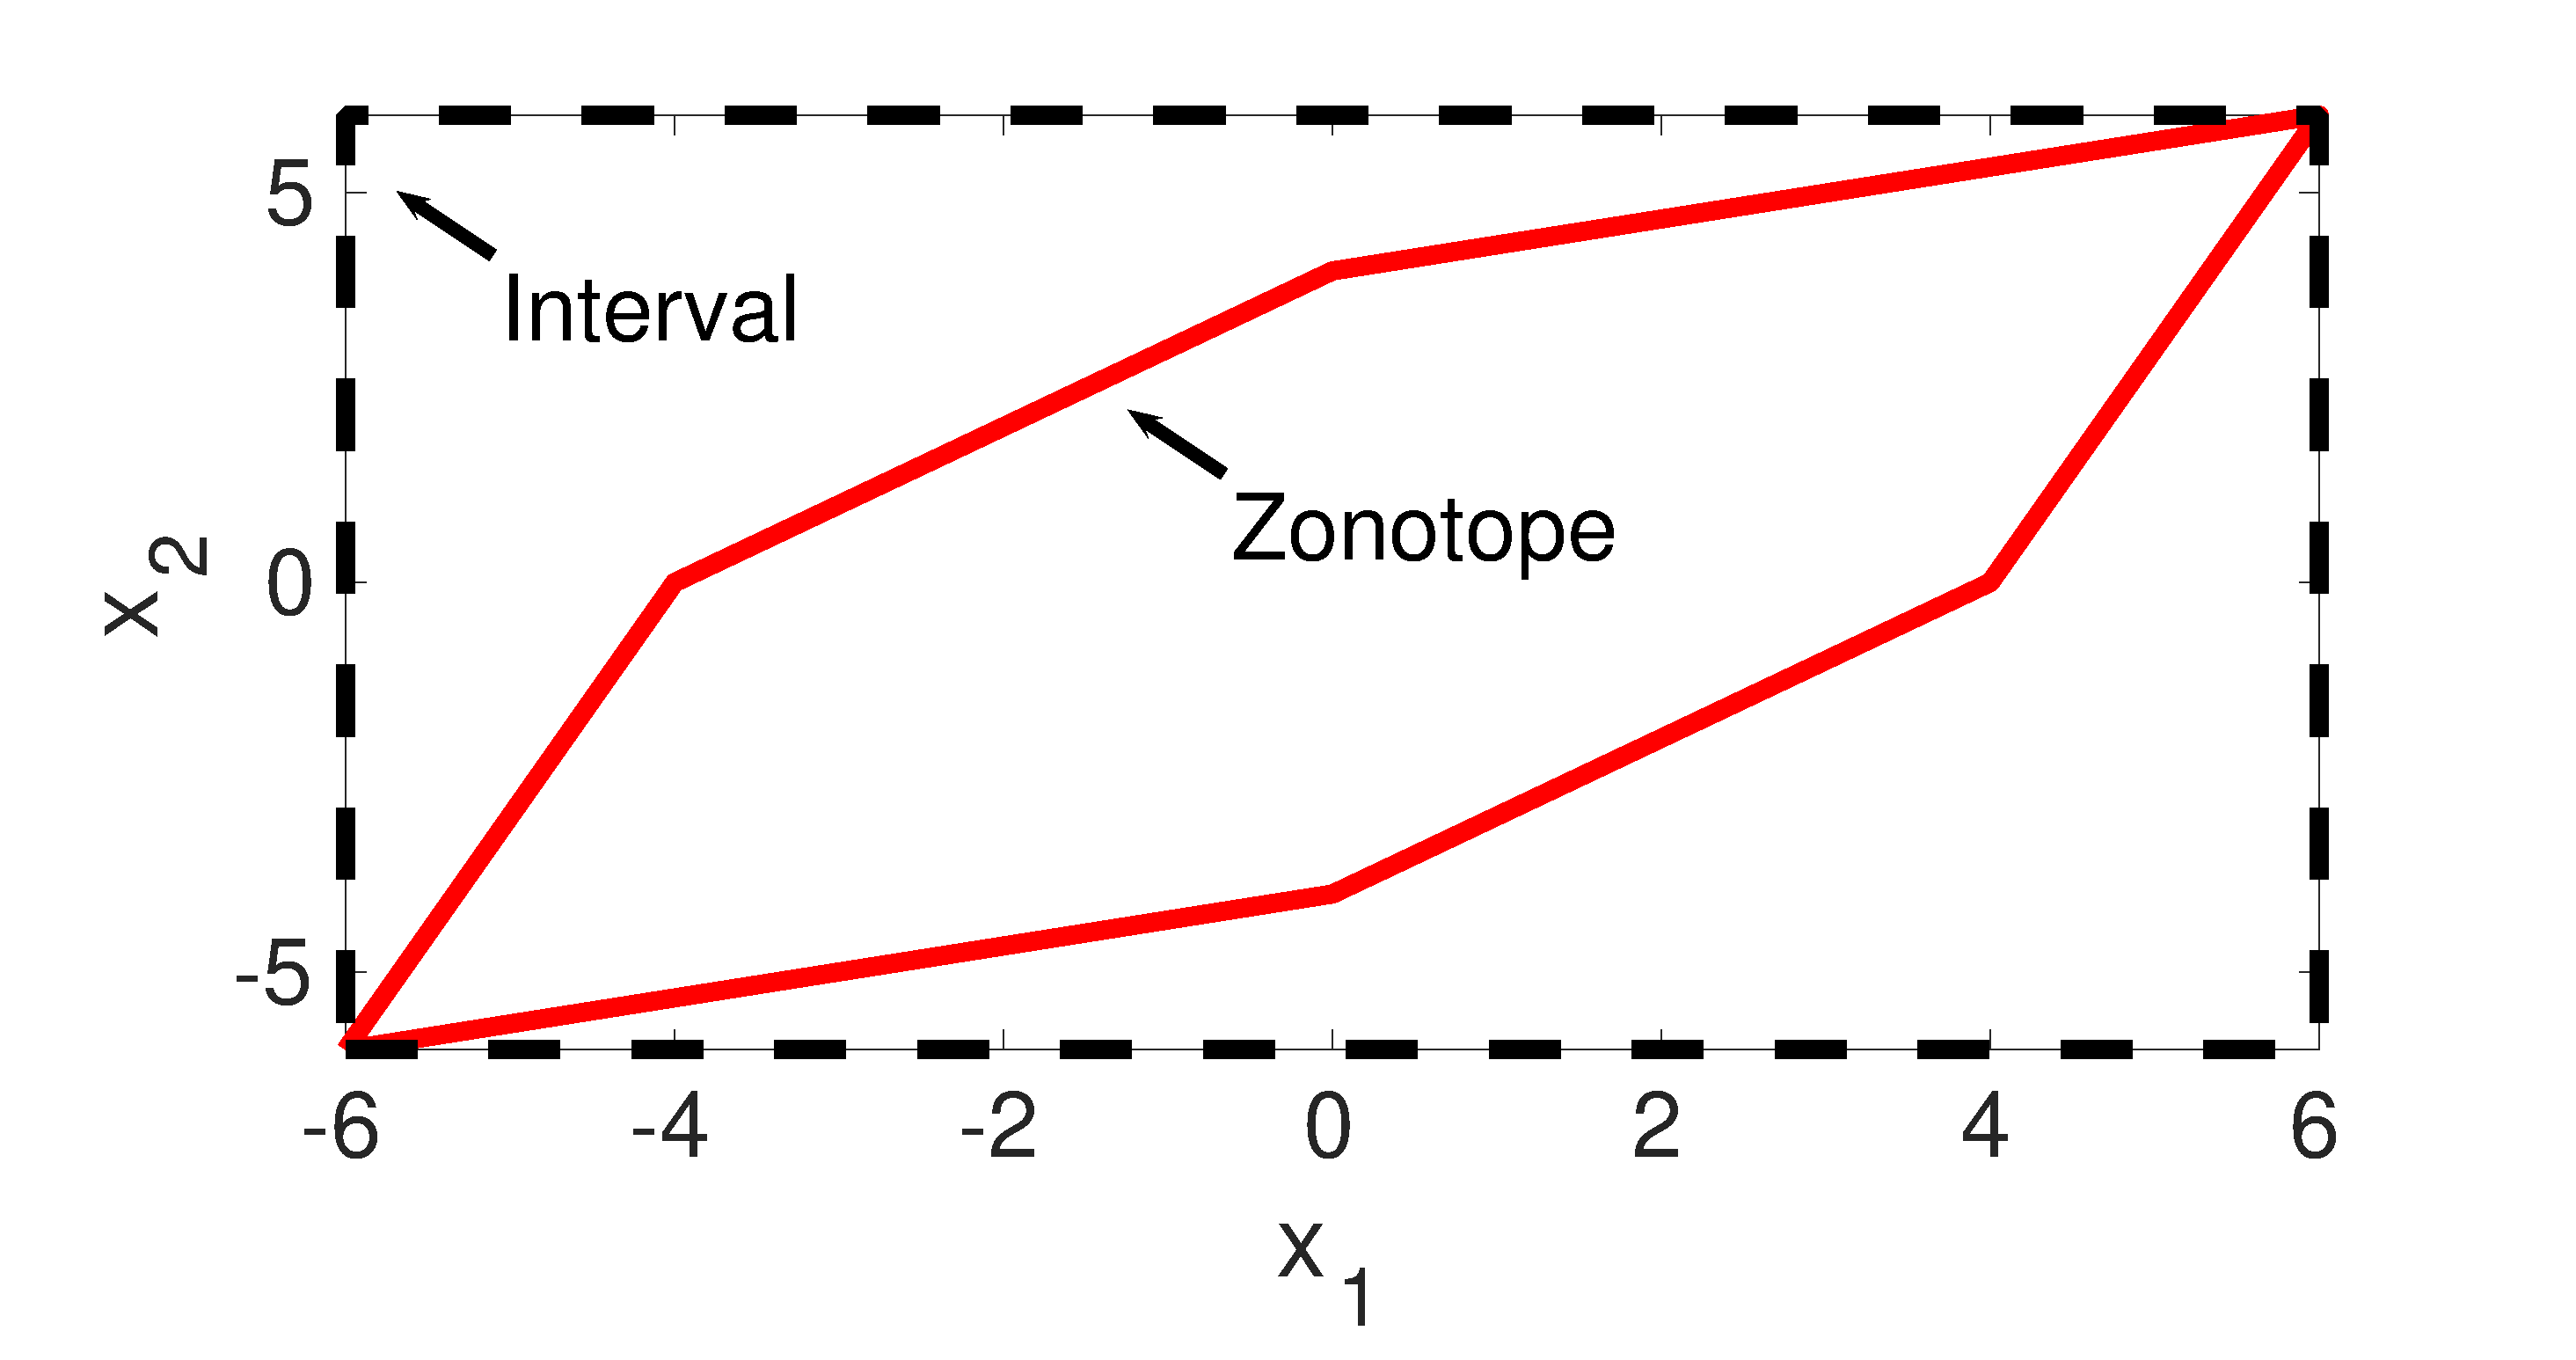
\includegraphics[scale=1, width=\linewidth]{figures/zonotope}
\caption{An illustration of a zonotope and its interval hull in 2-D}
\end{figure}
The construction, reduction, and interval calculation of zonotopes are implemented in the Matlab\textsuperscript{\tiny\textregistered} toolbox CORA (COntinuous Reachability Analyzer) \cite{Althoff2018}.
\section{Problem Formulation}
Let us denote the state of the vehicle to be tracked at time $k$ as $x_k$ and the measured state as $y_k$. Eq.~\eqref{formula:system} formuates a multi-output discrete-time linear system for the tracked vehicle, where $A, E \in \mathcal{R} ^{n_x \times n_x}$, $C \in \mathcal{R} ^{n_y \times n_x}$, and $F \in \mathcal{R} ^{n_y \times n_y}$ are matrices defined by the vehicle system model; $w_k$ and $v_k$ are process noise and measurement noise at time $k$, respectively. 
\begin{equation}
\label{formula:system}
\begin{split}
x_{k} &= Ax_{k-1} + Ew_k\\
y_k &= Cx_k + Fv_k
\end{split}
\end{equation}
Assuming $w_k$ and $v_k$ have known bounds ($\overline{w_k}$ and $\overline{v_k}$, respectively), we can define $\mathcal{W}$ and $\mathcal{V}$ such that $w_k \in \mathcal{W}$ and $v_k \in \mathcal{V}$ as \eqref{formula:wv}.
\begin{equation}
\label{formula:wv}
\mathcal{W} = \langle 0, H_w \rangle ,\quad \mathcal{V} = \langle 0, H_v \rangle
\end{equation}
The dimension of $x_k$ ($n_x$) varies across vehicle models; however, the measurement vector ($y_k$) is the measured position in the x and y-direction \eqref{formula:y}.  
\begin{equation}
\label{formula:y}
y =[ 
\begin{matrix}
s_x & s_y
\end{matrix}
]^T
\end{equation}
Given a vehicle model (discussed in the next section), the problem of set-based state estimation is to compute an outer bound of the state ($x_k$) containing all the possible values of the true state of the system consistent with the uncertain vehicle model and the measurements.
\section{Vehicle Model}
A major performance-influencing factor is to choose the right model for the tracked vehicle. Three linear systems are implemented in this paper to compare the state estimation algorithms. Although there exist highly precise vehicle models for ego vehicles, the simplest models are used here to represent the tracked vehicle, because complex vehicle models require parameters which are non-acquirable for tracked vehicles. In particular, physical dimensions, like wheelbase or side-slip, cannot be measured directly. Another reason is that adding some parameters, e.g. steering angle and yaw rate, makes the system non-linear and hence does not suit all the algorithms presented. Hence, the following models are investigated:
\begin{itemize}
\item \textbf{Constant Velocity (CV) Model}
\item \textbf{Constant Acceleration (CA) Model}
\item \textbf{Point-Mass (PM) Model}
\end{itemize}
\subsection{Constant Velocity Model}
The vehicle is assumed to travel in constant velocity \cite{Schubert2008}. The state of the system ($x_k$), state transition matrix ($A$), and the measurement matrix($C$) is shown in \eqref{formula:cvmodel}.
\begin{equation}
\label{formula:cvmodel}
\begin{split}
x &=
\left[\begin{matrix}
s_x & s_y & v_x & v_y
\end{matrix}\right]^{T}\\
A&= \left[\begin{matrix}
1 & 0 & \Delta T & 0\\
0 & 1 & 0 & \Delta T\\
0 & 0 & 1 & 0\\
0 & 0 & 0 & 1\\
\end{matrix}\right]\\
C&= \left[\begin{matrix}
1 & 0 & 0 & 0\\
0 & 1 & 0 & 0
\end{matrix}\right]
\end{split}
\end{equation}

\subsection{Constant Acceleration Model}
Although the constant velocity model is easy to implement, it is unrealistic to assume constant velocity. Acceleration model takes care of changing velocity and assumes constant acceleration \cite{Schubert2008}. Hence, the estimation errors for position and velocity are expected to be relatively smaller, when the velocity is constantly changing. The state of the system ($x_k$), the state transition matrix ($A$), and the measurement matrix($C$) are shown in \eqref{formula:camodel}.

\begin{equation}
\label{formula:camodel}
\begin{split}
x&= \left[\begin{matrix}
s_x & s_y & v_x & v_y & a_x & a_y
\end{matrix}\right]^{T}\\
A&= \left[\begin{matrix}
1 & 0 & \Delta T & 0 & \frac{1}{2}\Delta T^2 & 0\\
0 & 1 & 0 & \Delta T & 0 & \frac{1}{2}\Delta T^2 \\
0 & 0 & 1 & 0 & \Delta T & 0\\
0 & 0 & 0 & 1 & 0 & \Delta T\\
0 & 0 & 0 & 0 & 1 & 0\\
0 & 0 & 0 & 0 & 0 & 1
\end{matrix}\right] \\
C&= \left[\begin{matrix}
1 & 0 & 0 & 0 & 0 & 0\\
0 & 1 & 0 & 0 & 0 & 0
\end{matrix}\right]
\end{split}
\end{equation}

\subsection{Point-Mass Model}
It is trivial to note that vehicles might have varying acceleration, which is not satisfied in the previous models. This brings us to the point-mass model \cite{Althoff}, which is similar to the constant acceleration model, except that the acceleration here can strike up to a certain limit. This model treats the tracked vehicle as a point mass, ignoring wheel-base, slip-angle, etc. The state transition and measurement matrices are the same as the constant acceleration model (Eq.~\eqref{formula:camodel}). The acceleration bounds are set as $11.5 m/s^2$ \cite{Althoff} in both x and y-direction for this paper.

%\section{Domain Representation}
%The computation time of the algorithms largely varies due to the choice of shape to represent the set of state of the system. Zonotopes are gaining fame in the set-based state estimation techniques \cite{Le2013}, due to its control of wrapping effect and that the Minkowski sum of the zonotope results in zonotopes. The prediction step for the state estimation method can be simplified to basic matrix computation. The functionalities required in the correction step are implemented in the Matlab\textsuperscript{\tiny\textregistered} toolbox CORA (COntinuous Reachability Analyzer) \cite{Althoff2018}.
%
%Zonotopes are represented by a center, denoted by $p$ and generators, denoted by $H$. An m-zonotope in $\mathbb{R}^n$ can be defined as an affine transformation by $H$ of an m-dimensional hypercube in $\mathbb{R}^n$ centered at $p$. Minkowski sum, zonotope reduction, and the convex hull of zonotopes are required to be computed in the state estimation algorithms. The toolbox, CORA, is used to construct zonotopes and apply the computation for zonotopes in the algorithms. 
%\begin{figure}[!h]
%\label{fig:zonotope}
%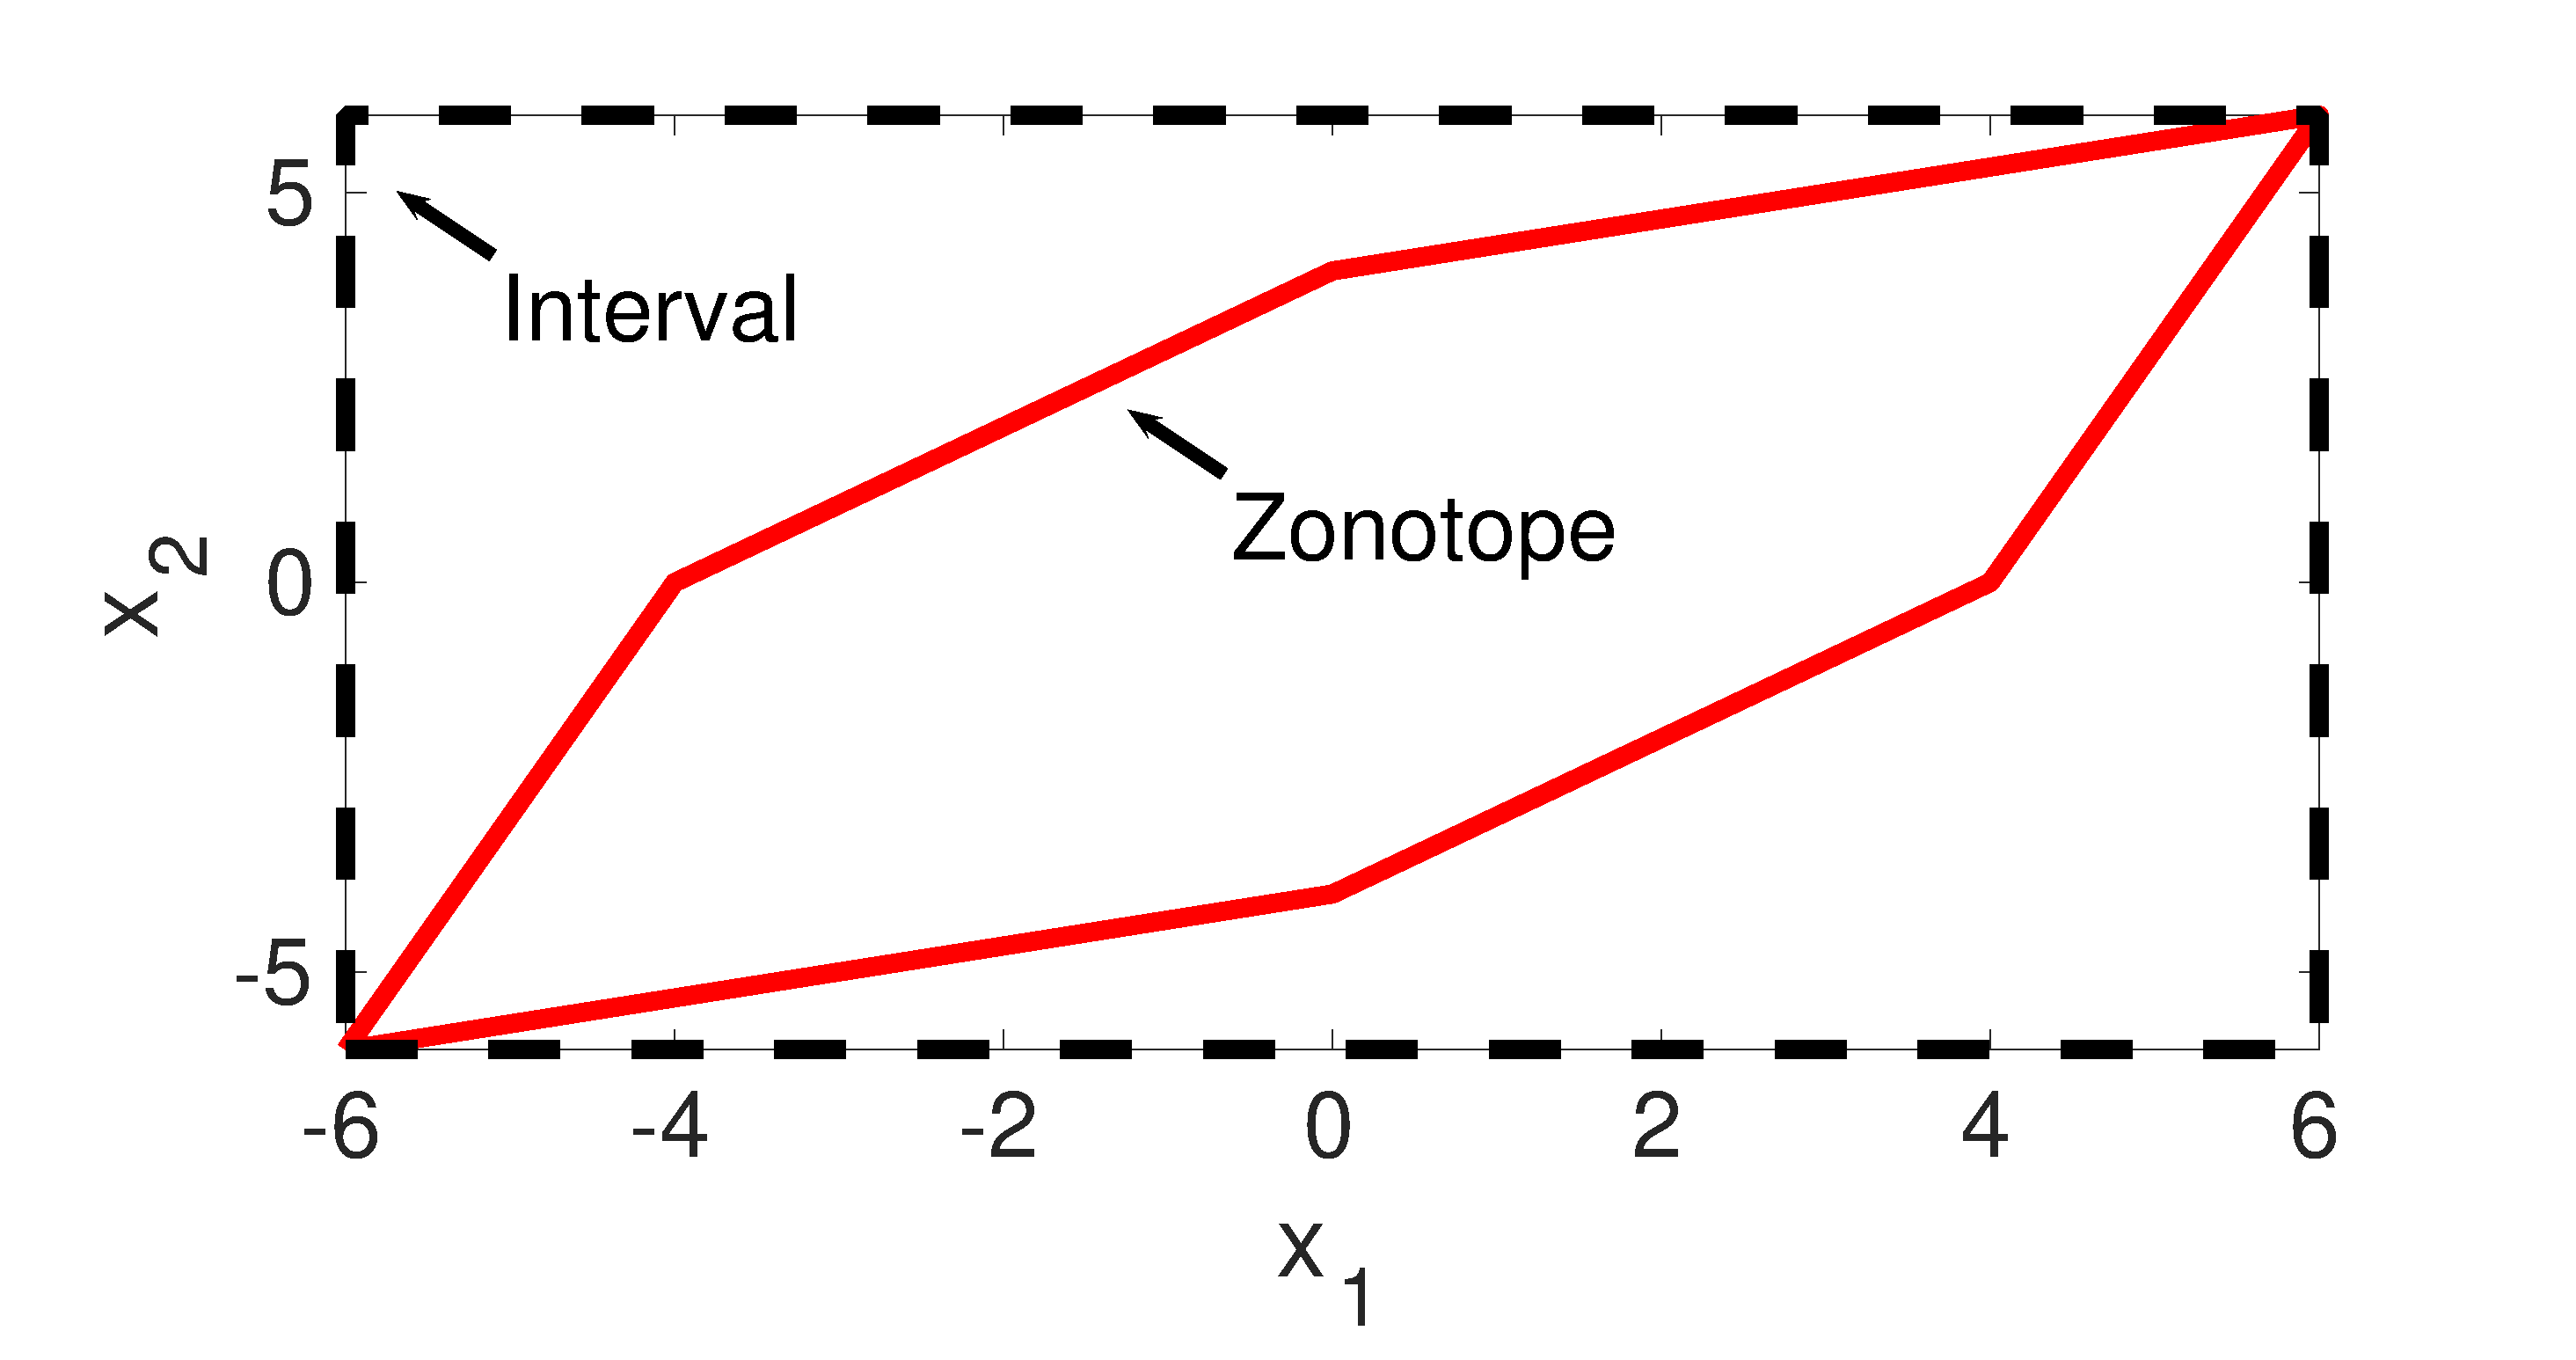
\includegraphics[scale=.25]{figures/zonotope}
%\caption{An illustration of a zonotope and its interval hull in 2-D}
%\end{figure}




\chapter{State Estimation} \label{ch:state_estimation}
State Estimation algorithms can be braodly classified into two types: Stochastic and Set-based algorithms. Stochastic state estimation algorithms assume that the uncertainties in the state of the system follow  a known probability distributions. It is difficult to fulfill the assumption for such algorithms, however, Zorzi \cite{Zorzi2017} proposed a family of Kalman Filter that solves the minimax problem with an iterative probability distribution of the uncertainties. Set-based algorithms, on the other hand, utilize geometrical sets as domain representation, like elipsoid or zonotope, to bound the possible sets of state of the system. Zonotopes are better than ellipsoids due to the balance of accuracy and computational cost. Furthermore, the zonotopes can control the wrapping effect \cite{Kuhn1998}, which is the term referred to the growth of the estimated state due to the propagated uncertainties in each iteration. Such algortithms can be further classified into segment intersection and interval observer. The former methods focus on intersecting the set of estimated state with the set of predicted state from the measurements. These methods try to minimize the bounds of the estimated state by using different properties of the geometric set like volume and radius. The interval observer methods, on the other hand, design observer to minimize the error on each time step. The following section digs deeper on the aforementioned methods.

\section{Segment Intersection} 
The predicted state of the system at a specific time and the previous state of the system are represented by zonotopes. The state estimated is the intersection of these zonotopes. Each algorithm tries to minimize the size of the intersected segment. Different properties of zonotopes, like P-radius and volume, are considered to represent the size of the segment. The following sections list and elaborates the algorithm that depends on different properties of zonotope.

\subsection{Frobenius norm of generators}
Frobenius norm of the generators of a zonotope is calculated using formula
\begin{equation}
||H||_{F}^2 = ||A + \lambda b^T||^{2}_F
\end{equation}
\begin{equation}
\label{lambdaformula}
\lambda^* = \frac{-Ab }{b^Tb}  = \frac{HH^Tc}{c^T HH^Tc} + \sigma^2
\end{equation}

The $\lambda$ that generates the minimum Frobenius norm of the generators of the intersected zonotope is calculated using the formula \ref{lambdaformula} for each iteration and the minimum zonotope is calculated.

\subsection{Volume}
The volume of a zonotope is calculated using the formula \ref{volumeformula}.
\begin{equation}
\label{volumeformula}
Vol(\hat{X}(\lambda)) = 2^n \sum^{N(n,r)}_{i=1} |1- c^T \lambda||det(A_i)| + 2^n \sum^{N(n-1,r)}_{i=1} \sigma|det[B_i \quad v_i]||v_i^T\lambda|
\end{equation}

\subsection{P-radius}
\begin{itemize}
\item TODO: Implement
\item TODO: Write
\end{itemize}

\section{Interval Observer}
\begin{itemize}
\item TODO: Write
\end{itemize}
\chapter{Result} \label{ch:result}
The INTERACTION Dataset \footnote{https://interaction-dataset.com/} is used to compare the algorithms and models of traffic participant tracking. The dataset contains multiple scenario in different locations where each scenario consists of multiple participants. Each participant is identified by an id for each scenario and each frame per 0.1s has a set of vehicles and their position. The x and y position of the vehicle is noted per time step and the algorithms aforementioned are applied to compare. The initial state of the system is set using assignments \ref{eq:initial}.
\begin{equation}
\label{eq:initial}
\begin{split}
x_0 &= zonotope([zeros(n), diag([1000;1000;10;10;10;10])])\\
w_k &= [0.1;0.1;0.4;0.4;0.1;0.1]\\
v_k &= [0.1;0.1]
\end{split}
\end{equation}

As seen from Fig. \ref{fig:segmentminimization}, the upper and lower bounds of the state estimation by Segment Minimization(using Frobenius norm) of the system bounds the true state. Comparing the error in different state of the system, as shown in Fig. \ref{fig:comparison}, suggests that both the algorithm requires around 0.5s to converge to near the true state. Interesting to note, the Interval Estimation has a higher error peak compared to Segment Minimization using the same dataset.\\

The Fig. \ref{fig:histogram} shows the Histogram of RMSE of estimation from Segment Minimization. The errors are calculated after 10 seconds in order to avoid the initial peak. The histograms suggest that, the method gives little error for estimating the measured state, whereas, for unmeasured state like velocity, the error is at most twice the true state.

\begin{figure}[h!]
\begin{subfigure}{.5\textwidth}
\centering
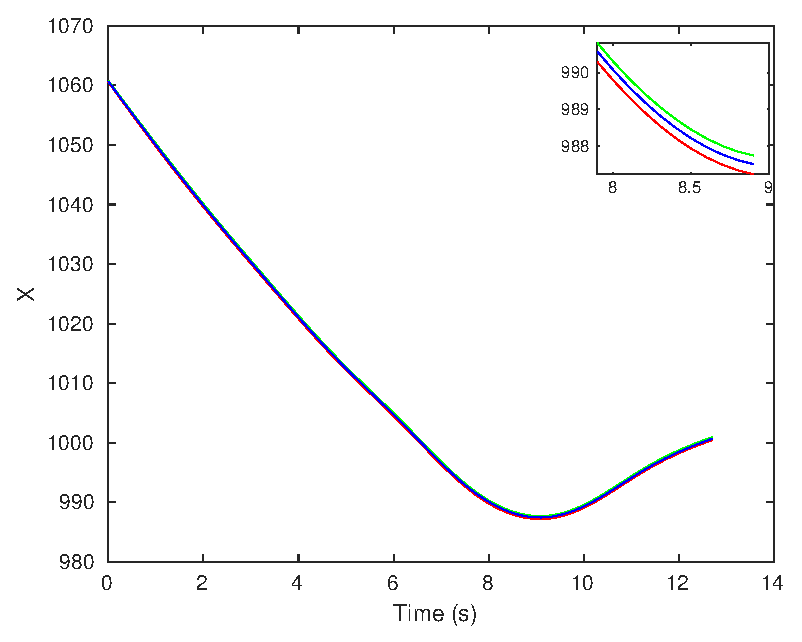
\includegraphics[width=.8\linewidth]{figures/s_caXzoomed}
\caption{Estimating $x$}
\end{subfigure}
\begin{subfigure}{.5\textwidth}
\centering
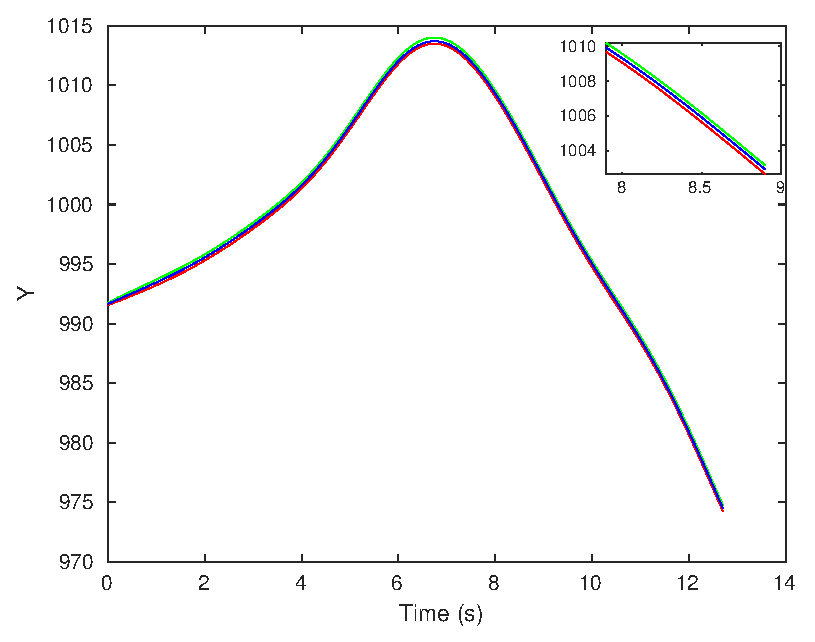
\includegraphics[width=.8\linewidth]{figures/s_caYzoomed}
\caption{Estimating $y$}
\end{subfigure}
\begin{subfigure}{.5\textwidth}
\centering
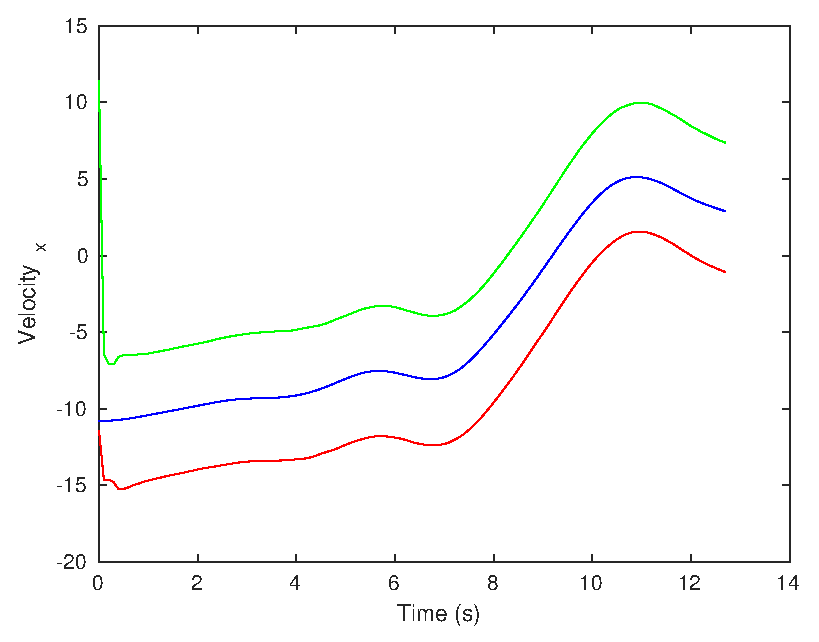
\includegraphics[width=.8\linewidth]{figures/s_caVelocity_x}
\caption{Estimating $velocity_x$}
\end{subfigure}
\begin{subfigure}{.5\textwidth}
\centering
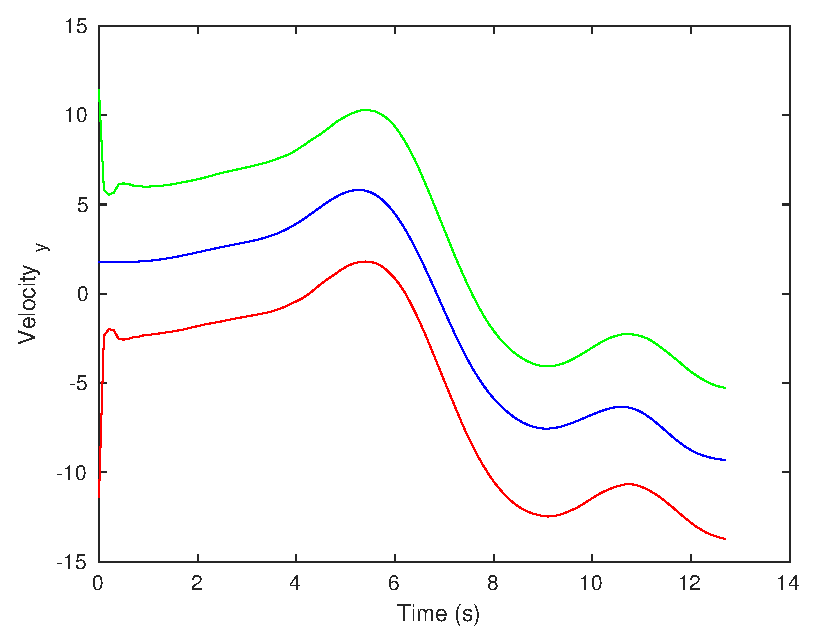
\includegraphics[width=.8\linewidth]{figures/s_caVelocity_y}
\caption{Estimating $velocity_y$}
\end{subfigure}
{\color{red}\rule{.1\linewidth}{1pt}} : Lower bound of estimation\\
{\color{green}\rule{.1\linewidth}{1pt}} : Upper bound of estimation\\
{\color{blue}\rule{.1\linewidth}{1pt}} : True value
\caption{Segment Minimization using Frobenius norm}
\label{fig:segmentminimization}
\end{figure}

\begin{figure}[h!]
\begin{subfigure}{.5\textwidth}
\centering
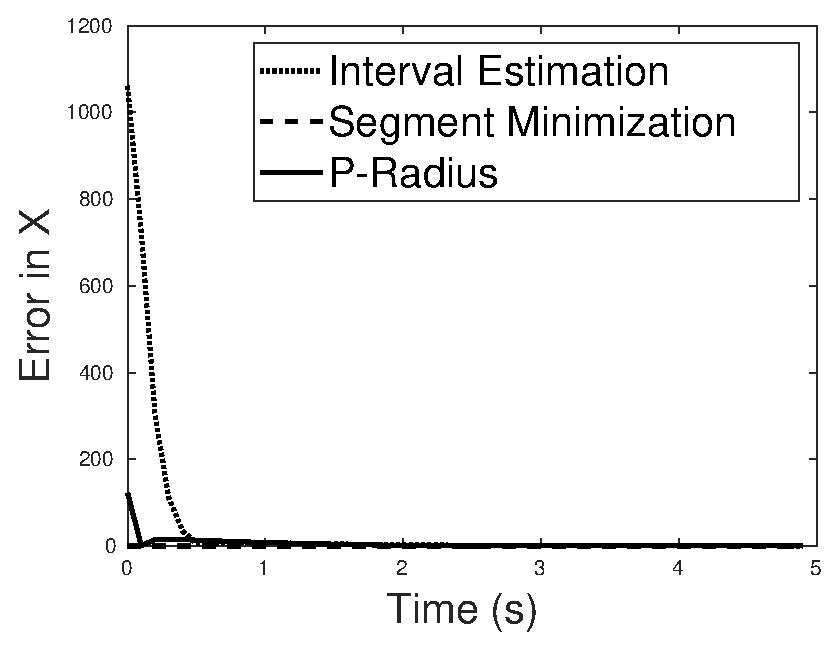
\includegraphics[width=.8\linewidth]{figures/errorsX}
\caption{Error in $x$}
\end{subfigure}
\begin{subfigure}{.5\textwidth}
\centering
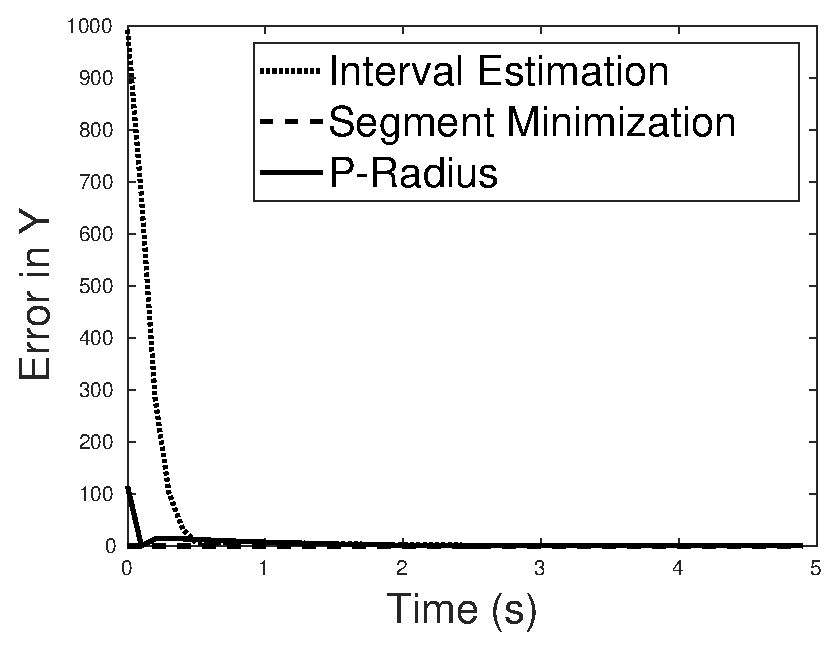
\includegraphics[width=.8\linewidth]{figures/errorsY}
\caption{Error in $y$}
\end{subfigure}
\begin{subfigure}{.5\textwidth}
\centering
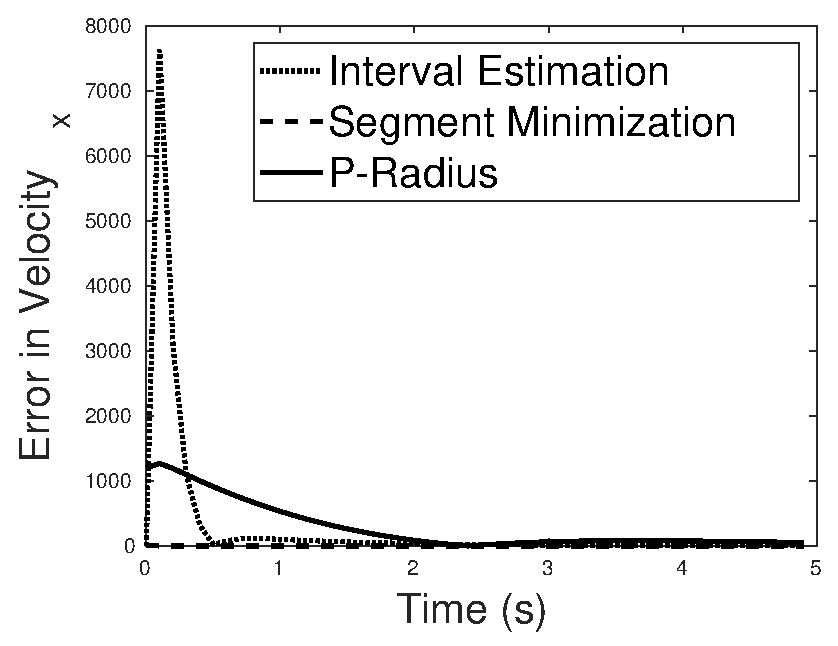
\includegraphics[width=.8\linewidth]{figures/errorsVelocity_x}
\caption{Error in $velocity_x$}
\end{subfigure}
\begin{subfigure}{.5\textwidth}
\centering
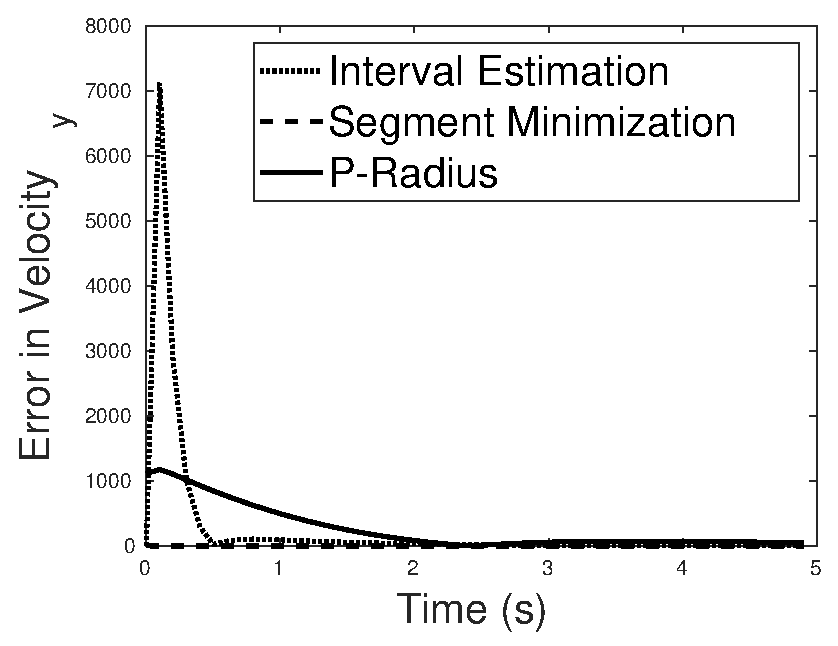
\includegraphics[width=.8\linewidth]{figures/errorsVelocity_y}
\caption{Error in  $velocity_y$}
\end{subfigure}
\caption{Comparing error from different algorithms on same dataset}
\label{fig:comparison}
\end{figure}


\begin{figure}[h!]
\begin{subfigure}{.5\textwidth}
\centering
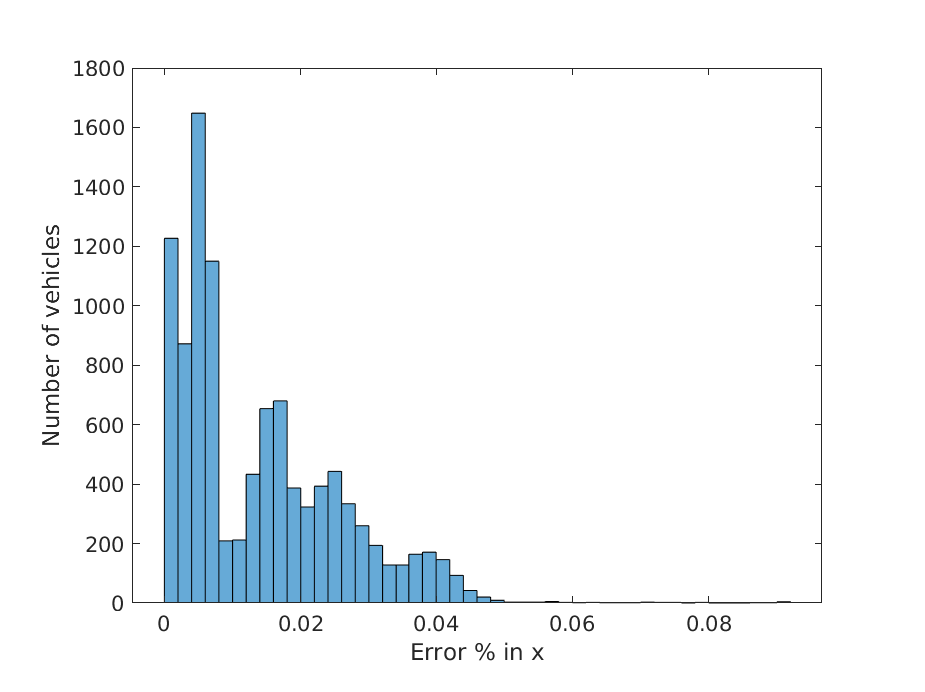
\includegraphics[width=.8\linewidth]{figures/s_caXerror}
\caption{RMSE $x$}
\end{subfigure}
\begin{subfigure}{.5\textwidth}
\centering
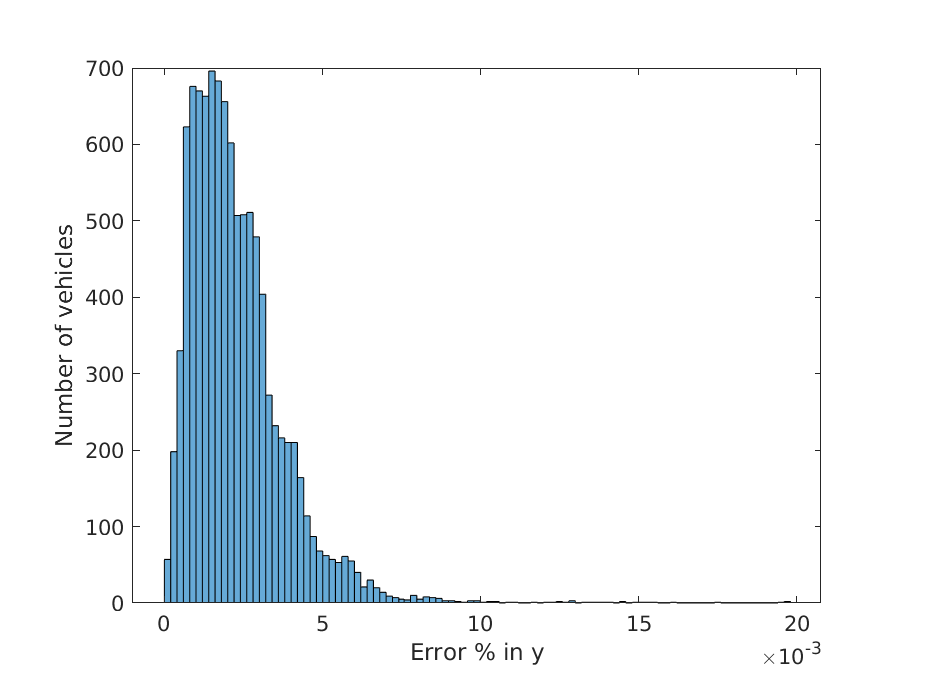
\includegraphics[width=.8\linewidth]{figures/s_caYerror}
\caption{RMSE $y$}
\end{subfigure}
\begin{subfigure}{.5\textwidth}
\centering
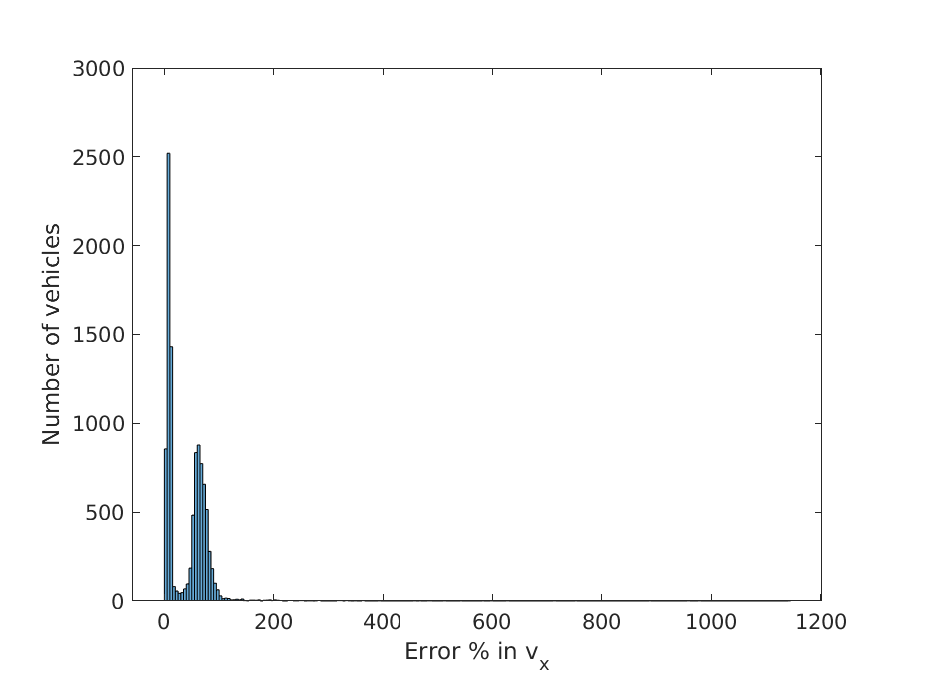
\includegraphics[width=.8\linewidth]{figures/s_cavXerror}
\caption{RMSE in $velocity_x$}
\end{subfigure}
\begin{subfigure}{.5\textwidth}
\centering
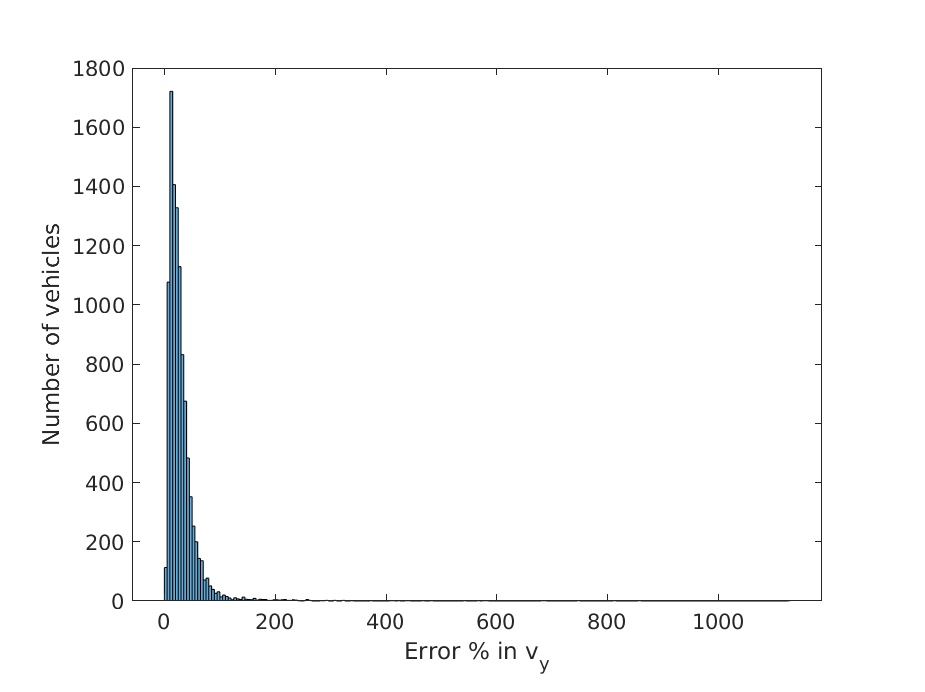
\includegraphics[width=.8\linewidth]{figures/s_cavYerror}
\caption{RMSE in $velocity_y$}
\end{subfigure}
\caption{Histogram of errors from Segment Minimizer on 651 vehicles }
\label{fig:histogram}
\end{figure}
%\begin{itemize}
%\item{Efficiency}
%\item{Accuracy}
%\item{Performance Metric}

\chapter{Conclusion} \label{ch:conclusion}
A demand for intelligent collision avoidance system is timeless. To take load off sensors and hardware of a vehicle, state estimation algorithms can be used to track vehicle and estimate properties required for collision-free path prediction. On comparing multiple techniques using different models to represent the tracked vehicle, it can be concluded that the segment minimization using F-radius gives a good trade-off between fast convergence, accuracy and tight bound. H-$\infty$ and segment minimization using P-radius are ahead in terms of computation time because these methods carry out computation off-line before any input measurement, and hence as a consequence over-approximates and does not improvise estimation significantly for each measurement. Choice of model to represent the state of the system also has significant effect on the performance. To estimate velocity, constant velocity model gives better results, whereas for acceleration, the point mass model gives better estimate compared to the constant acceleration model. This paper can be a starting point to implement higher defined models of tracked vehicle and compare performance of state estimation methods. The state estimation methods can further be evaluated on implementing with distinguishable set of initial starting state to determine the effect of initial estimation on the algorithms, if any. Further developments can include implementing the technique in real vehicle system and using the estimation to track vehicles.

\appendix{}
\chapter{Extended Results} \label{ch:eresult}
\section{Set Estimation}
\FloatBarrier
\subsection{Segment Minimization using F-Radius}
\begin{figure}[!h]
\begin{subfigure}{.5\linewidth}
\centering
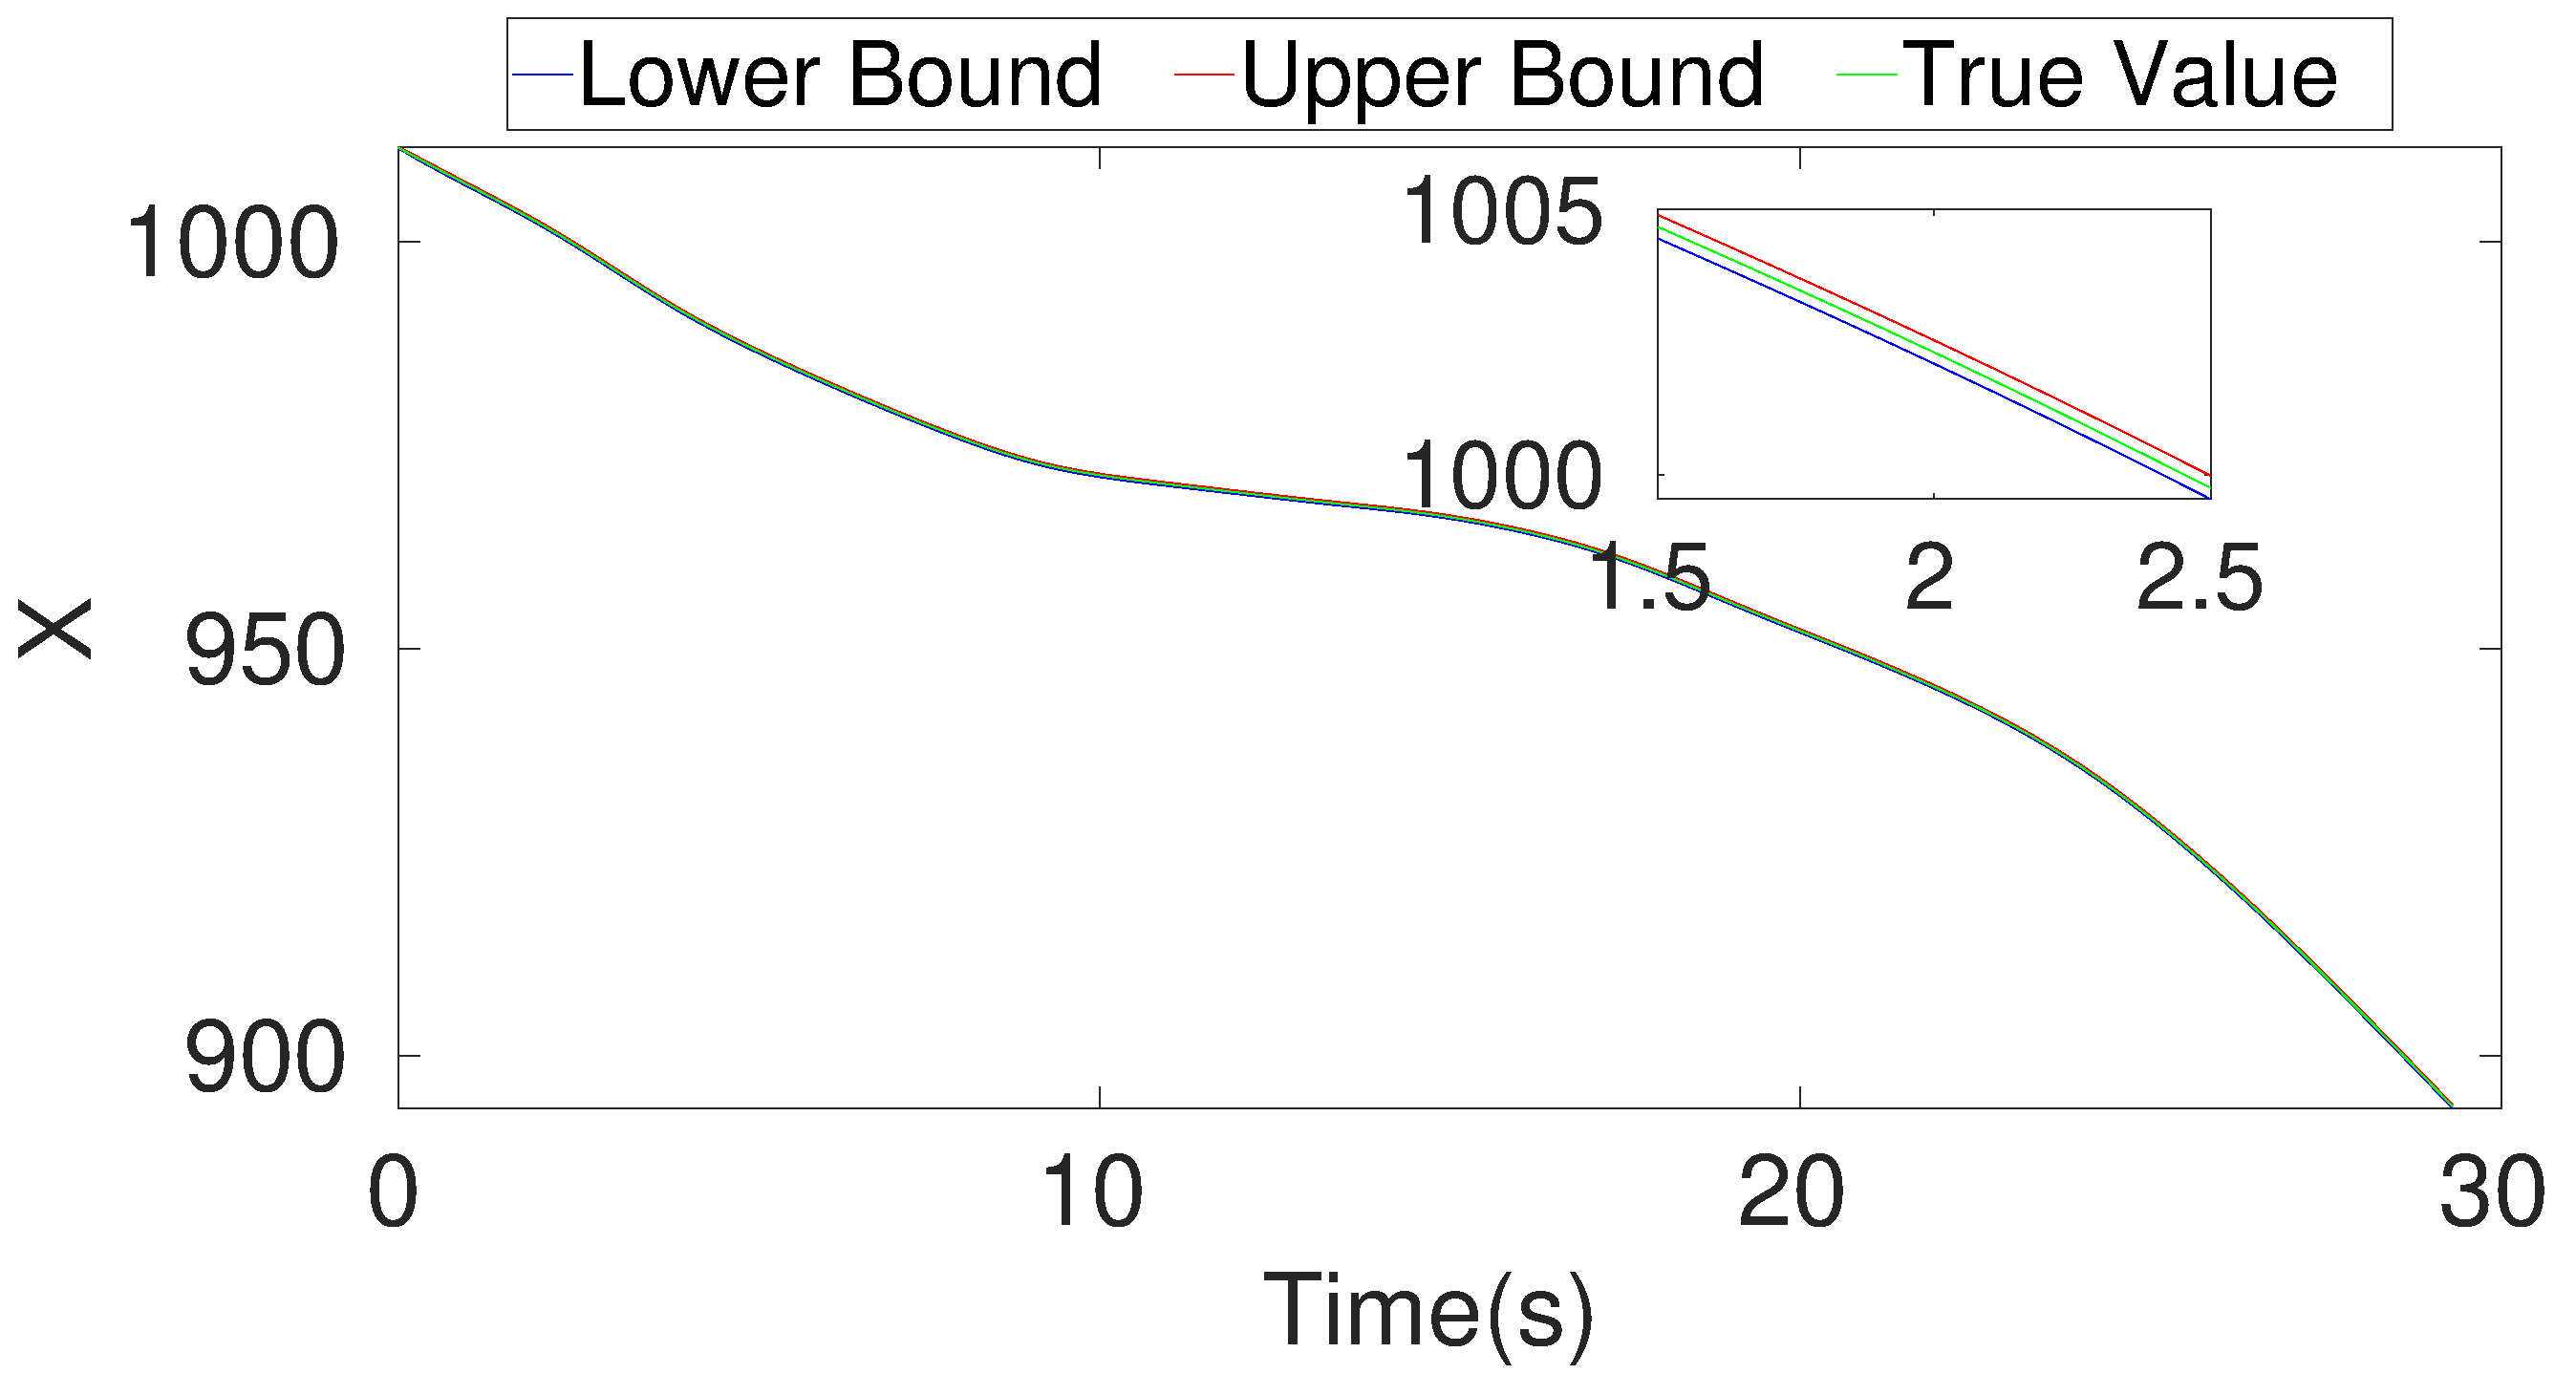
\includegraphics[width=\linewidth]{figures/Frad/s3cvSMX}
\end{subfigure}
\begin{subfigure}{.5\linewidth}
\centering
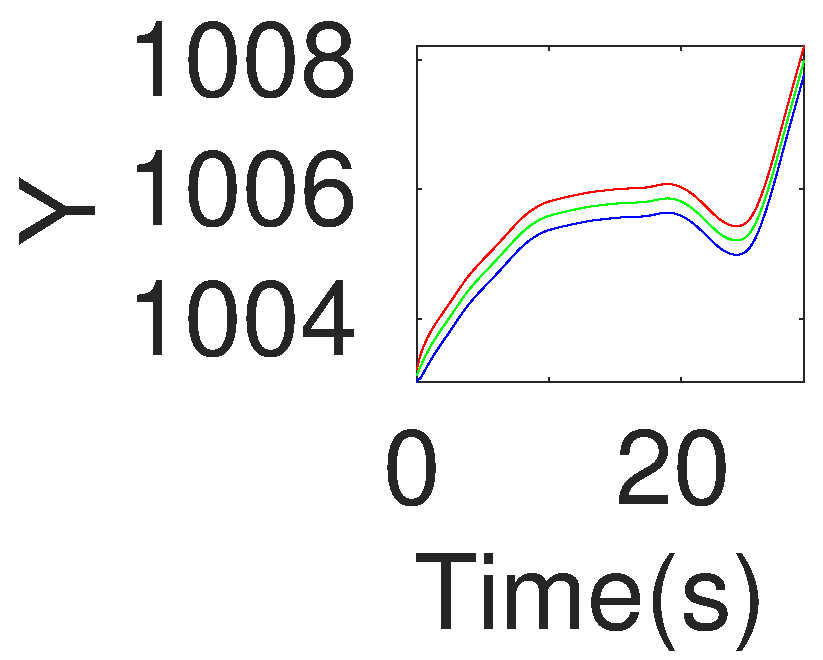
\includegraphics[width=\linewidth]{figures/Frad/s3cvSMY}
\end{subfigure}
\begin{subfigure}{.5\linewidth}
\centering
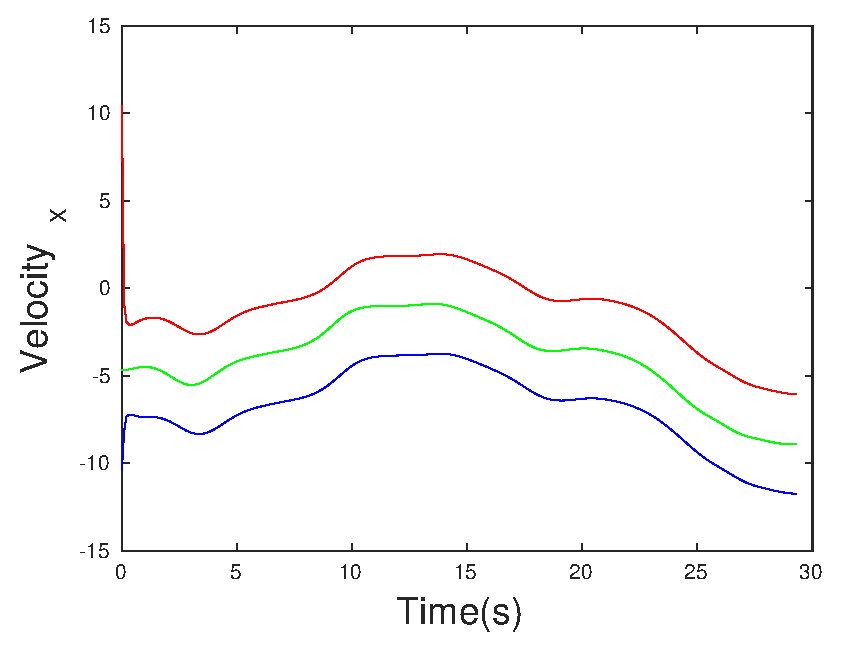
\includegraphics[width=.9\linewidth]{figures/Frad/s3cvSMVelocity_x}
\end{subfigure}
\begin{subfigure}{.5\linewidth}
\centering
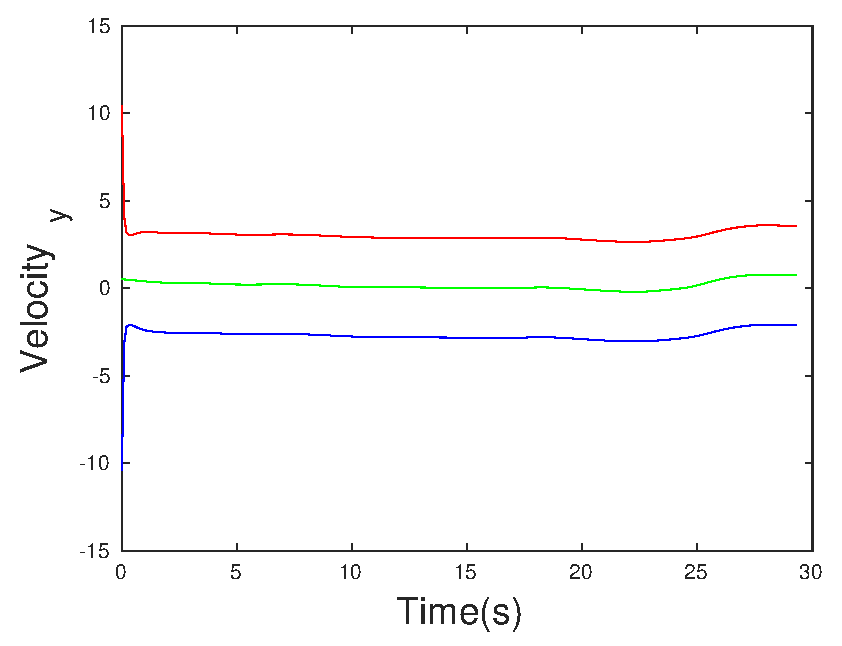
\includegraphics[width=.9\linewidth]{figures/Frad/s3cvSMVelocity_y}
\end{subfigure}
\caption{Estimation using Constant Velocity}
\end{figure}

\begin{figure}[!h]
\begin{subfigure}{.5\linewidth}
\centering
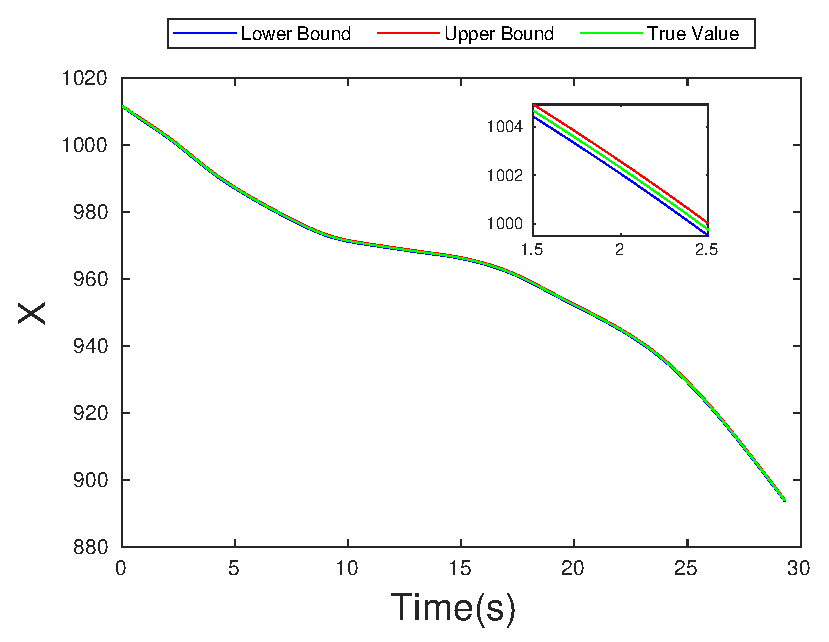
\includegraphics[width=\linewidth]{figures/Frad/s3caSMX}
\end{subfigure}
\begin{subfigure}{.5\linewidth}
\centering
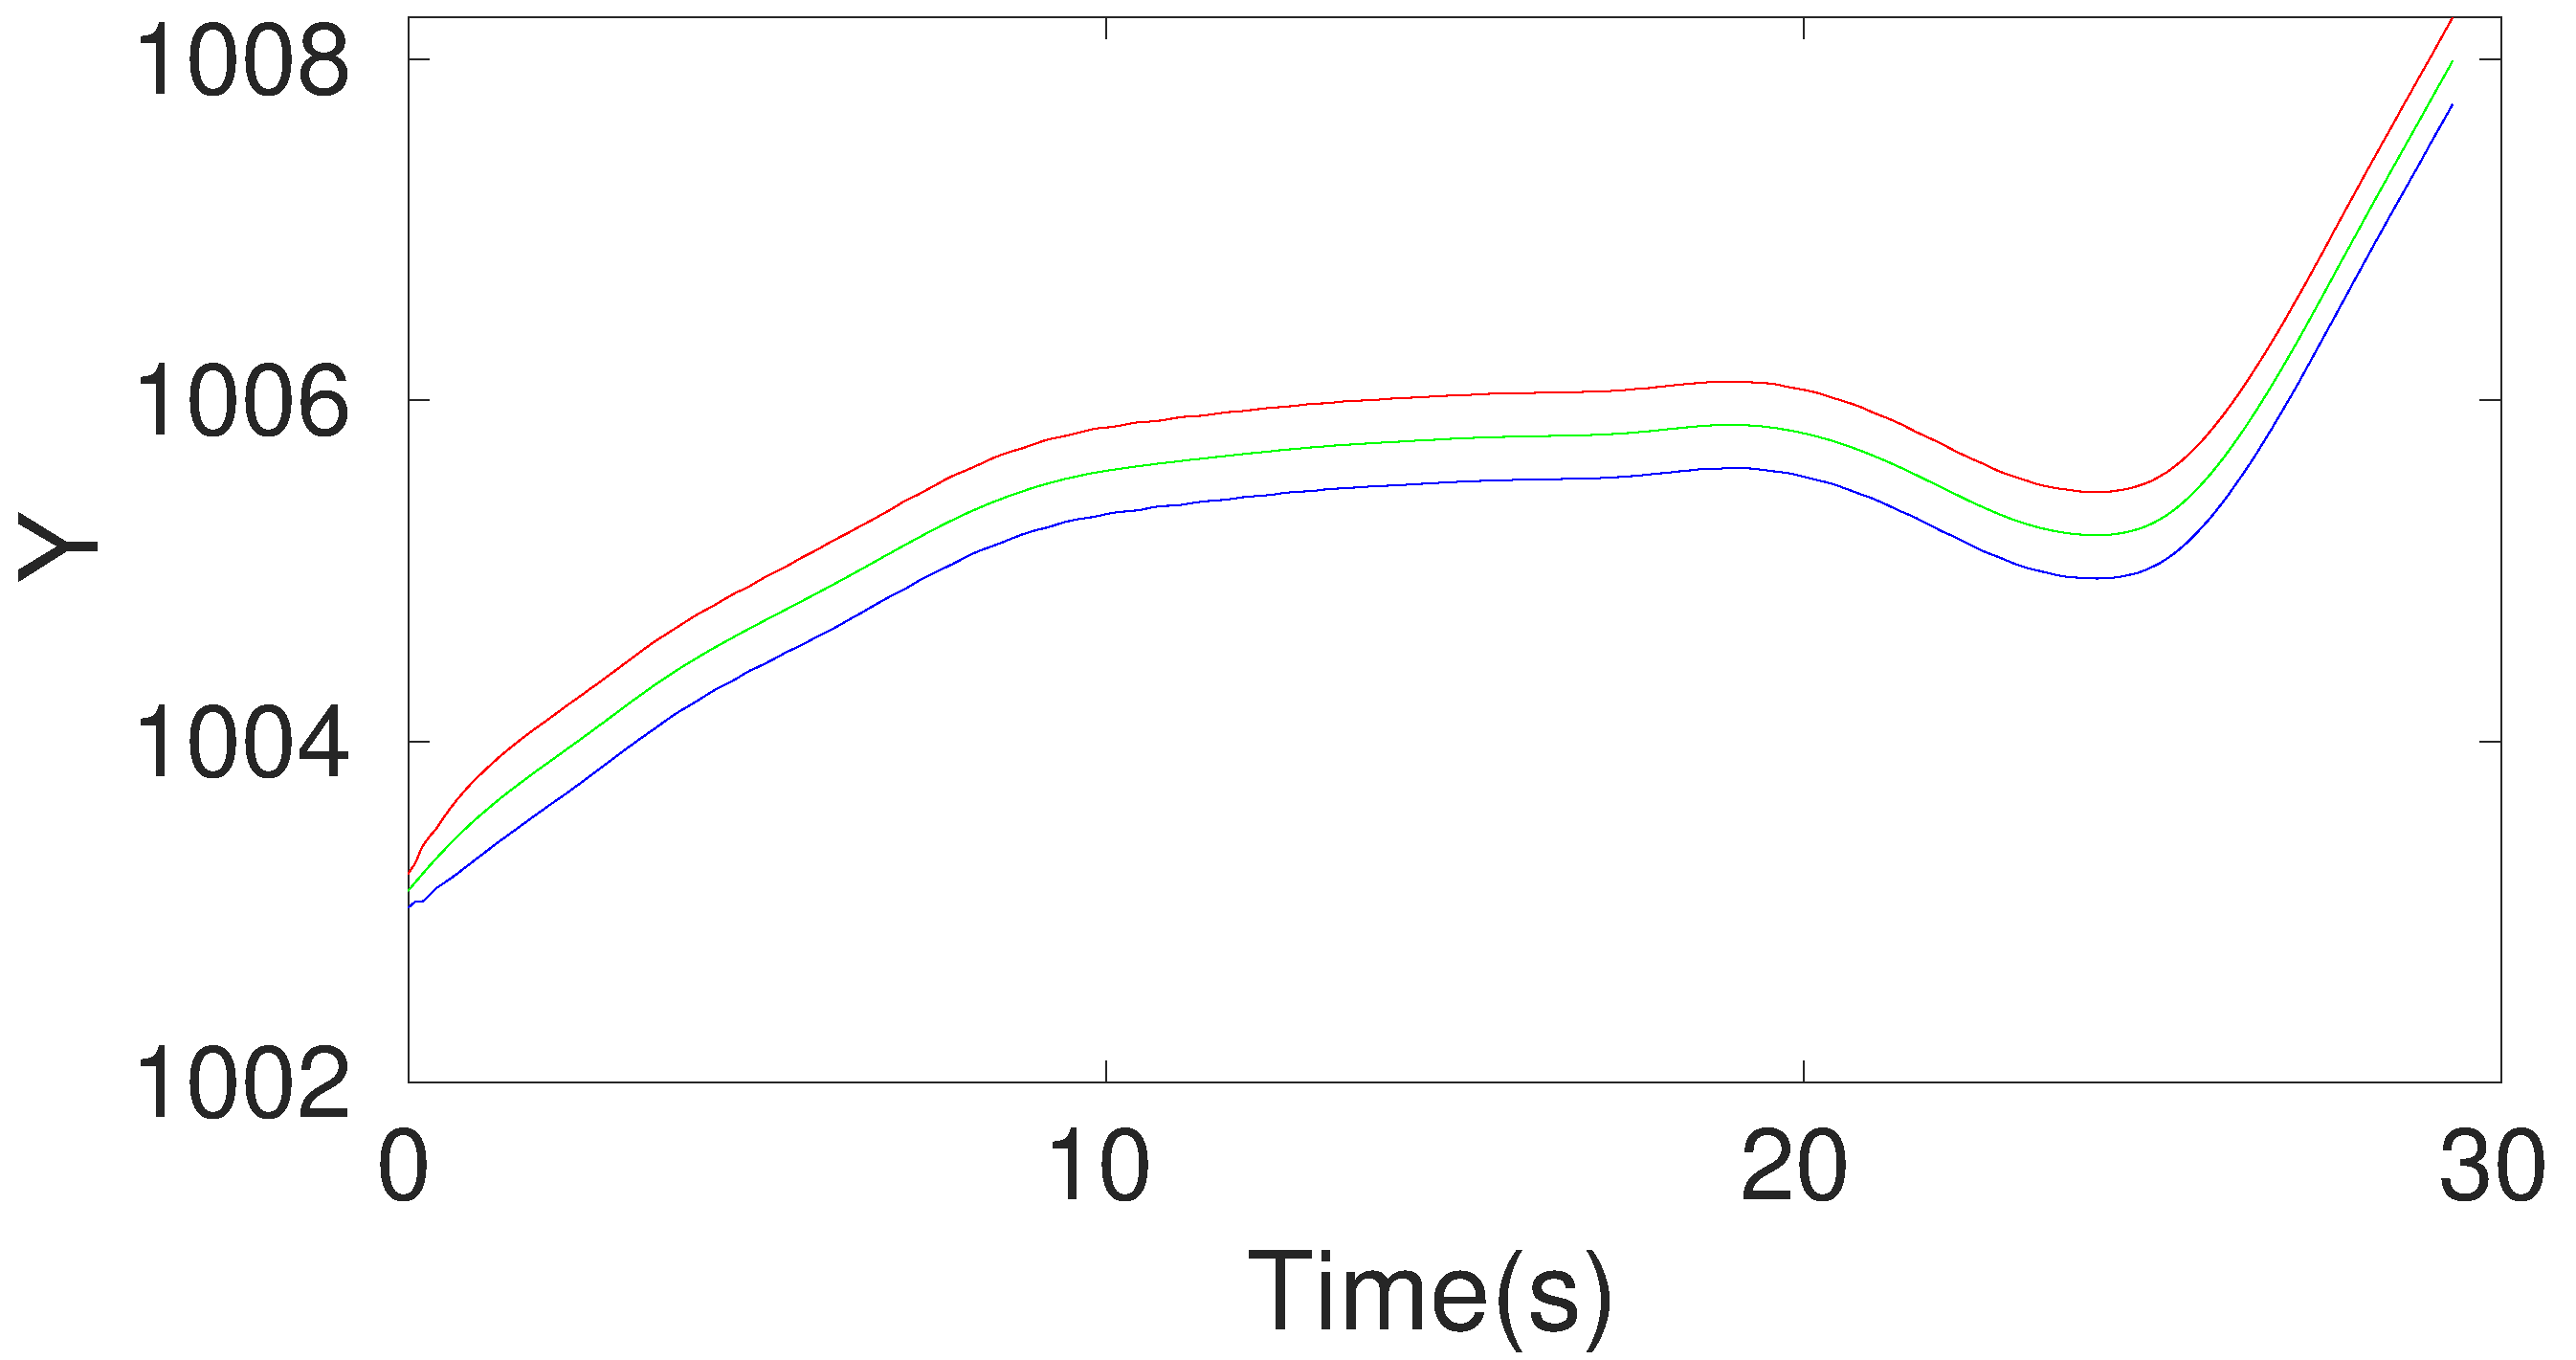
\includegraphics[width=\linewidth]{figures/Frad/s3caSMY}
\end{subfigure}
\begin{subfigure}{.5\linewidth}
\centering
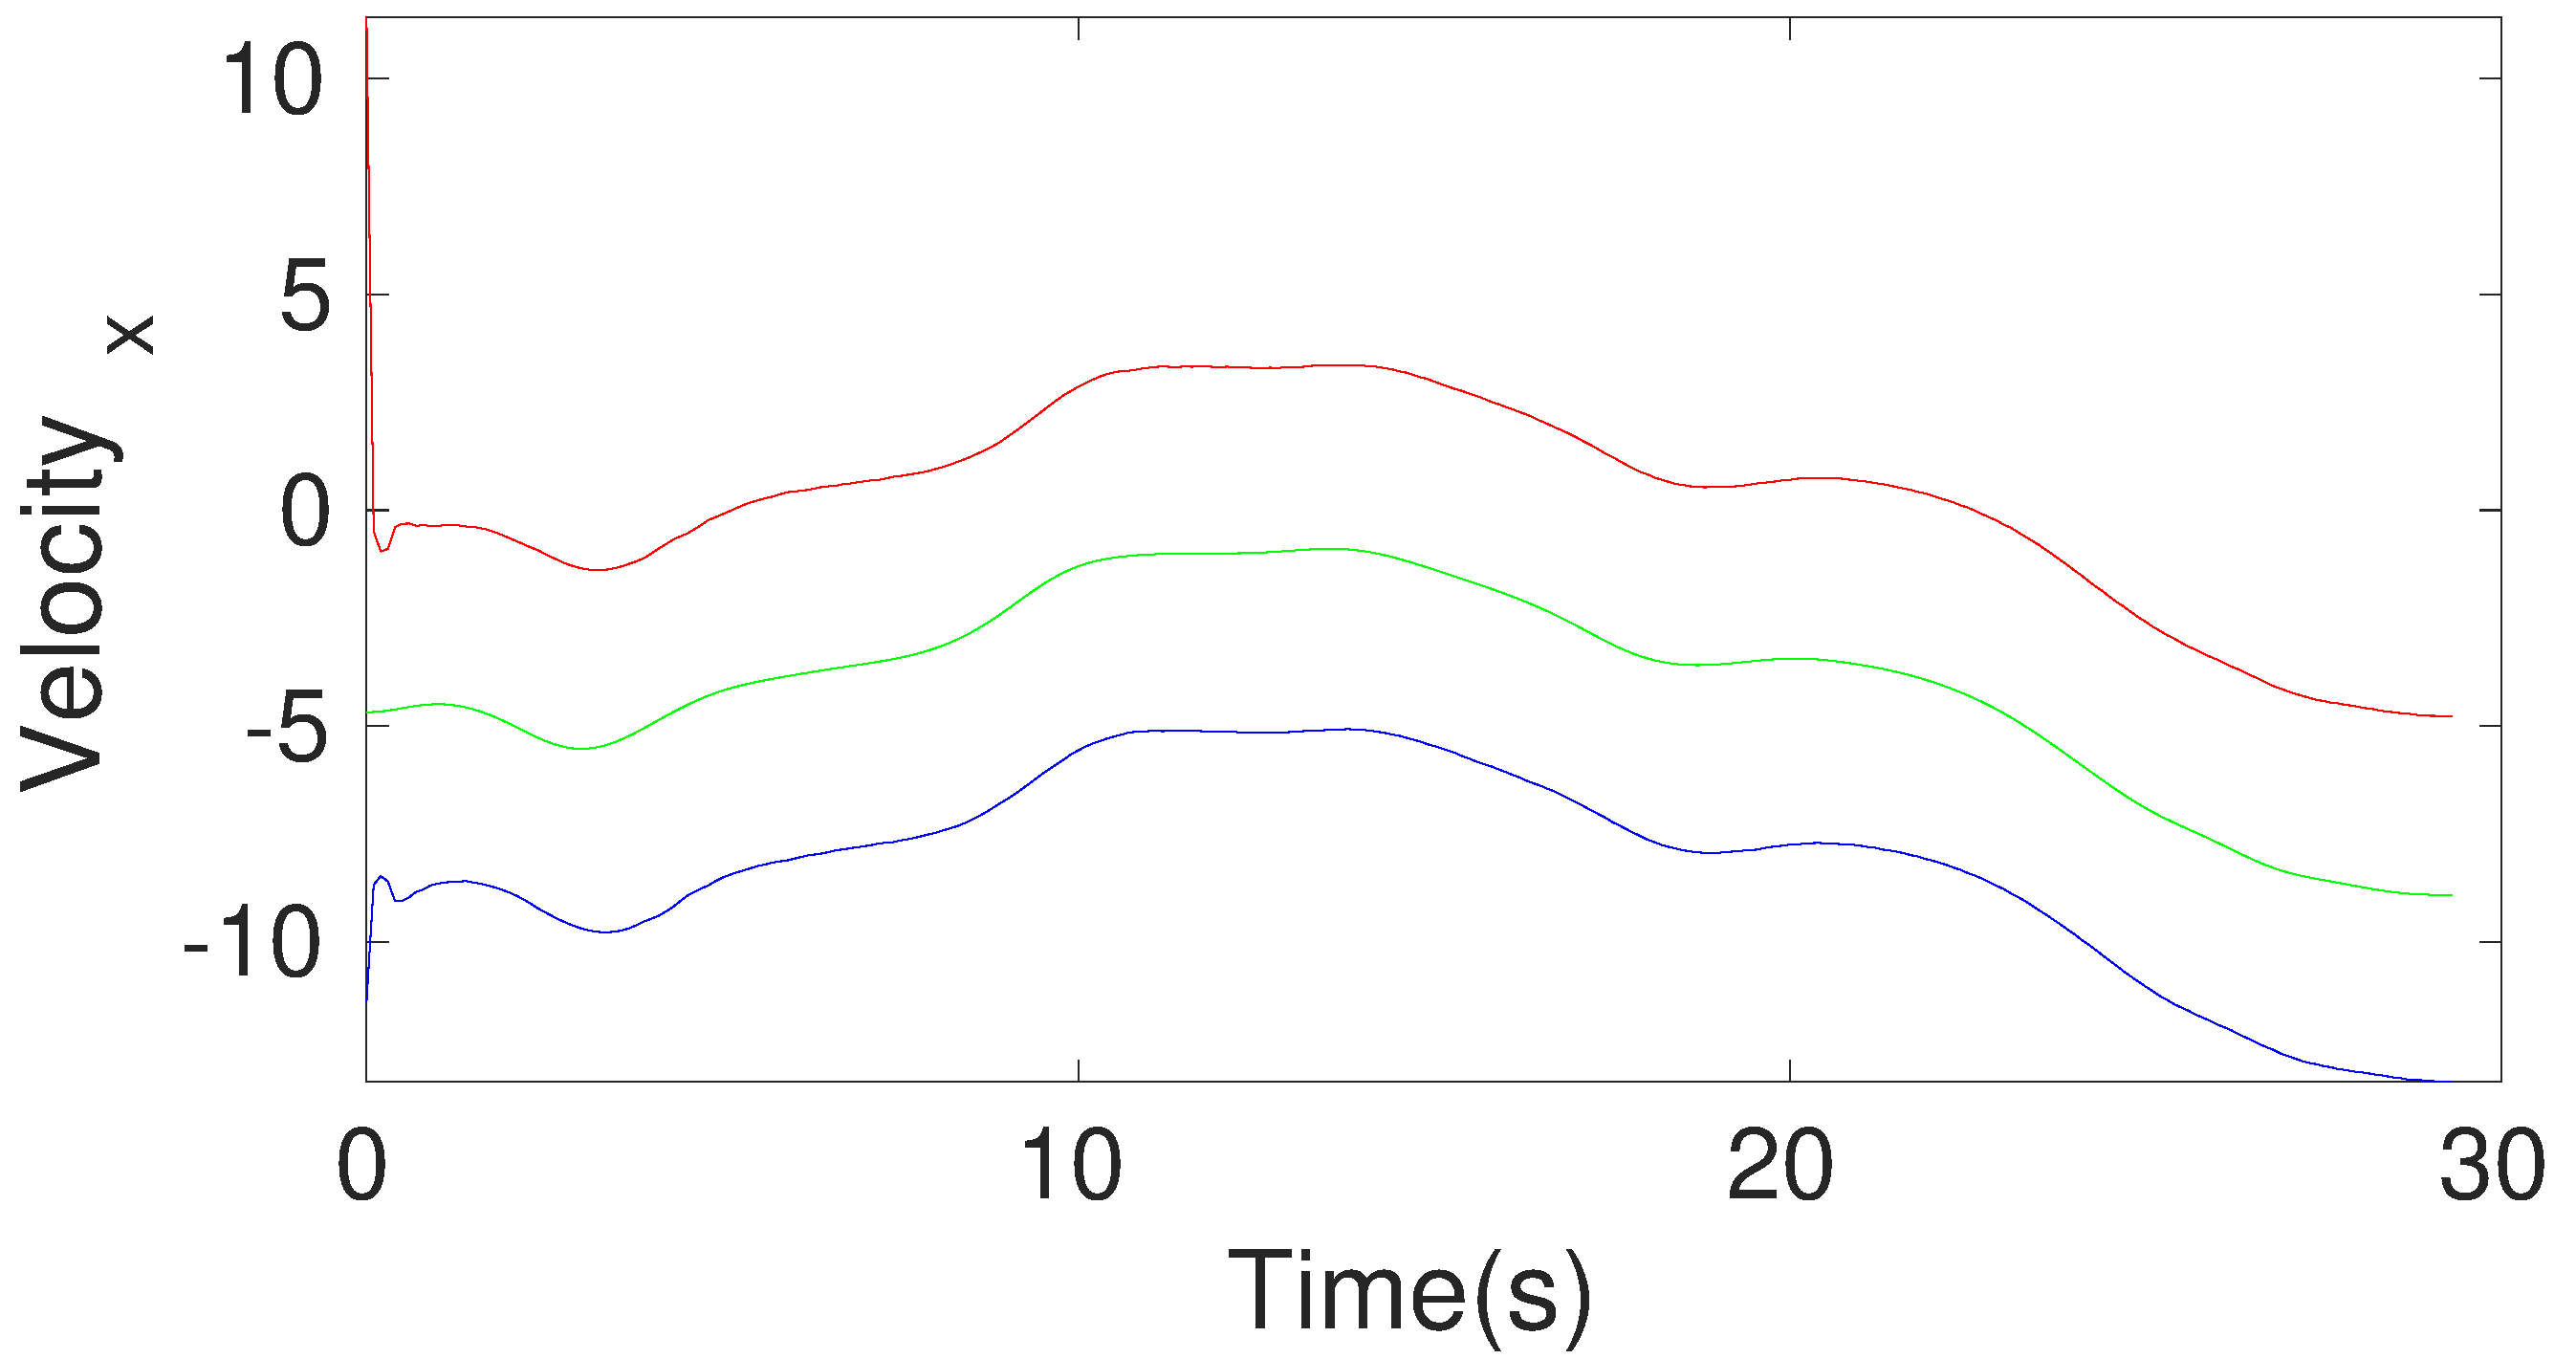
\includegraphics[width=.9\linewidth]{figures/Frad/s3caSMVelocity_x}
\end{subfigure}
\begin{subfigure}{.5\linewidth}
\centering
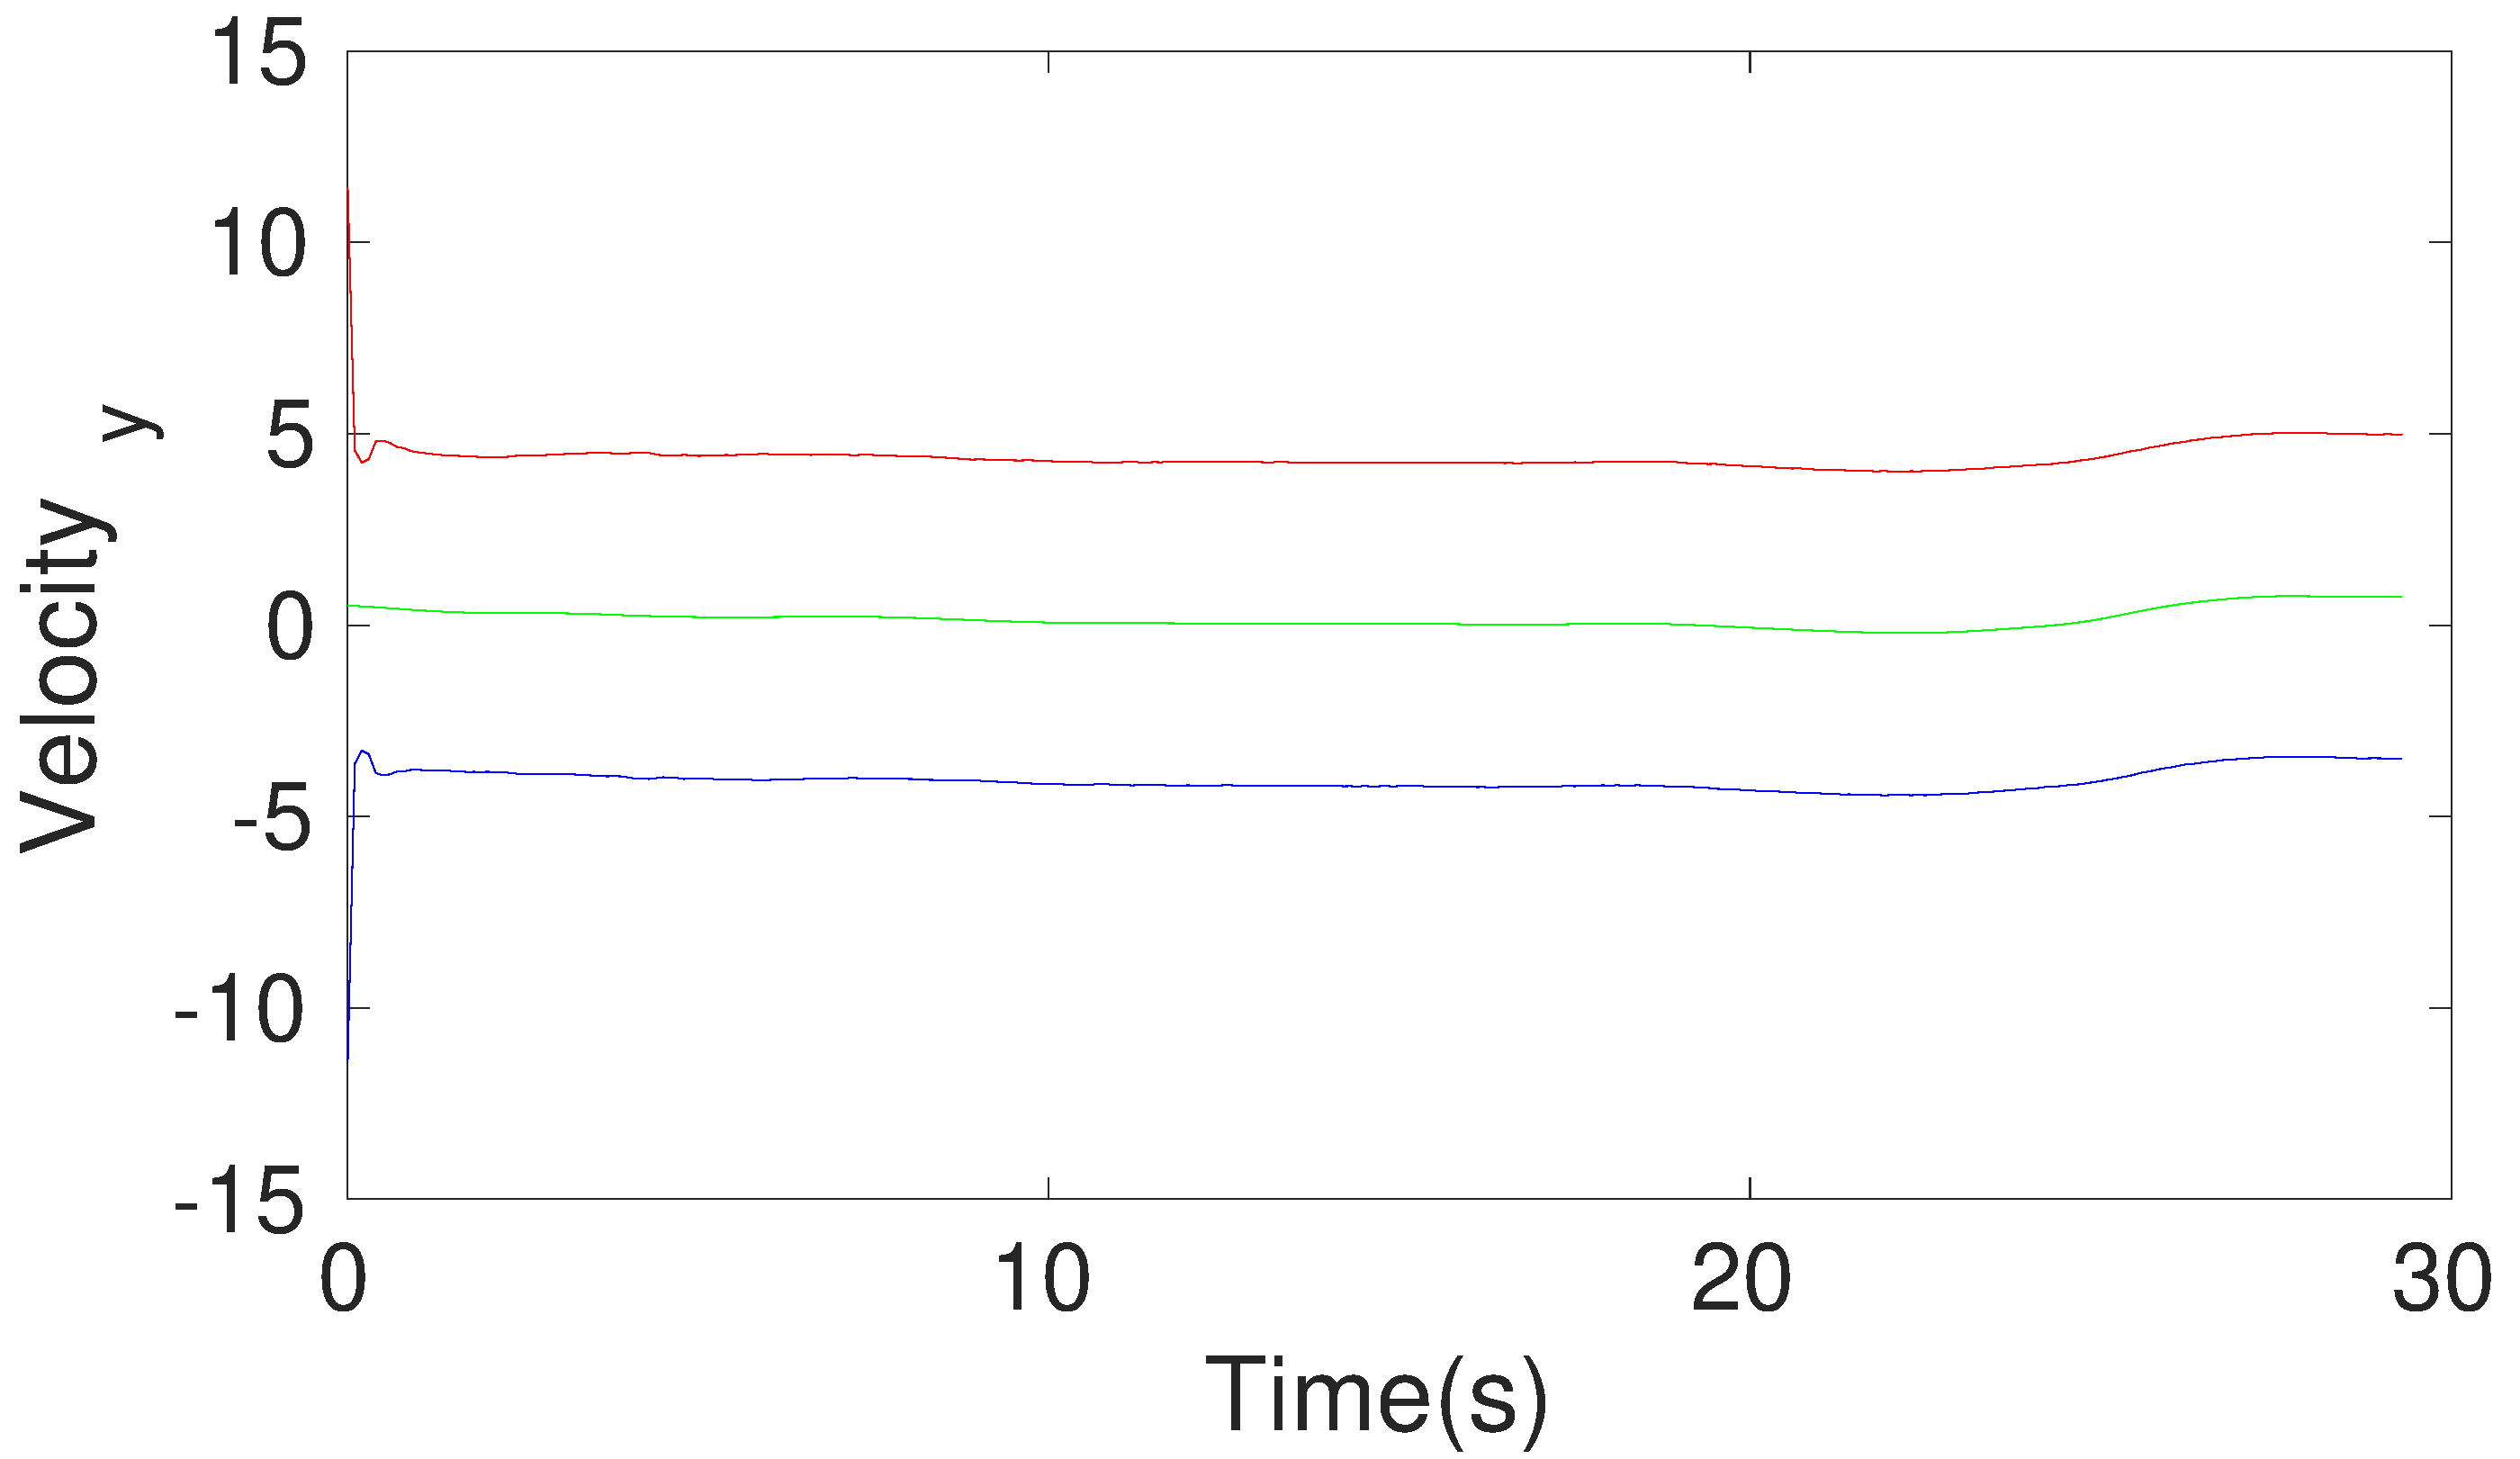
\includegraphics[width=.9\linewidth]{figures/Frad/s3caSMVelocity_y}
\end{subfigure}
\begin{subfigure}{.5\linewidth}
\centering
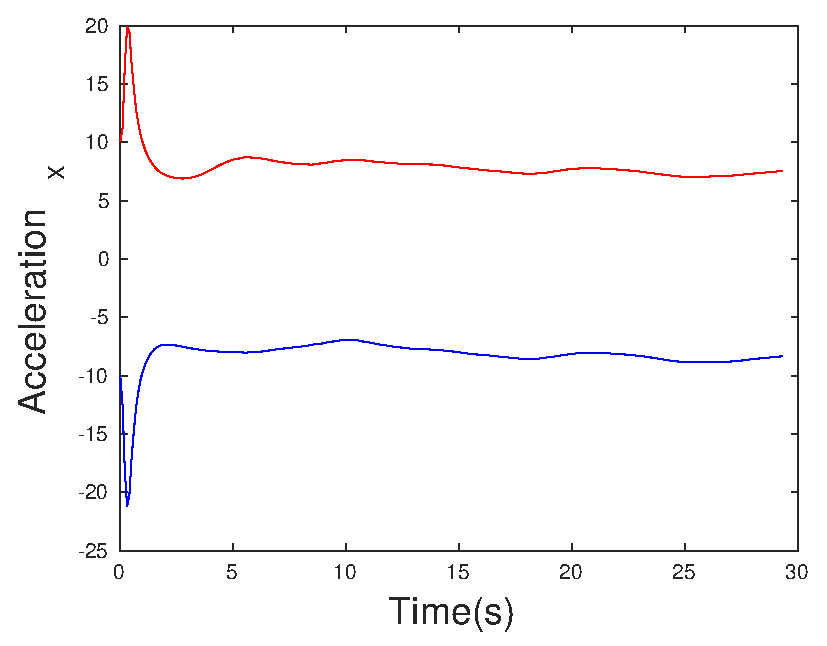
\includegraphics[width=.9\linewidth]{figures/Frad/s3caSMAcceleration_x}
\end{subfigure}
\begin{subfigure}{.5\linewidth}
\centering
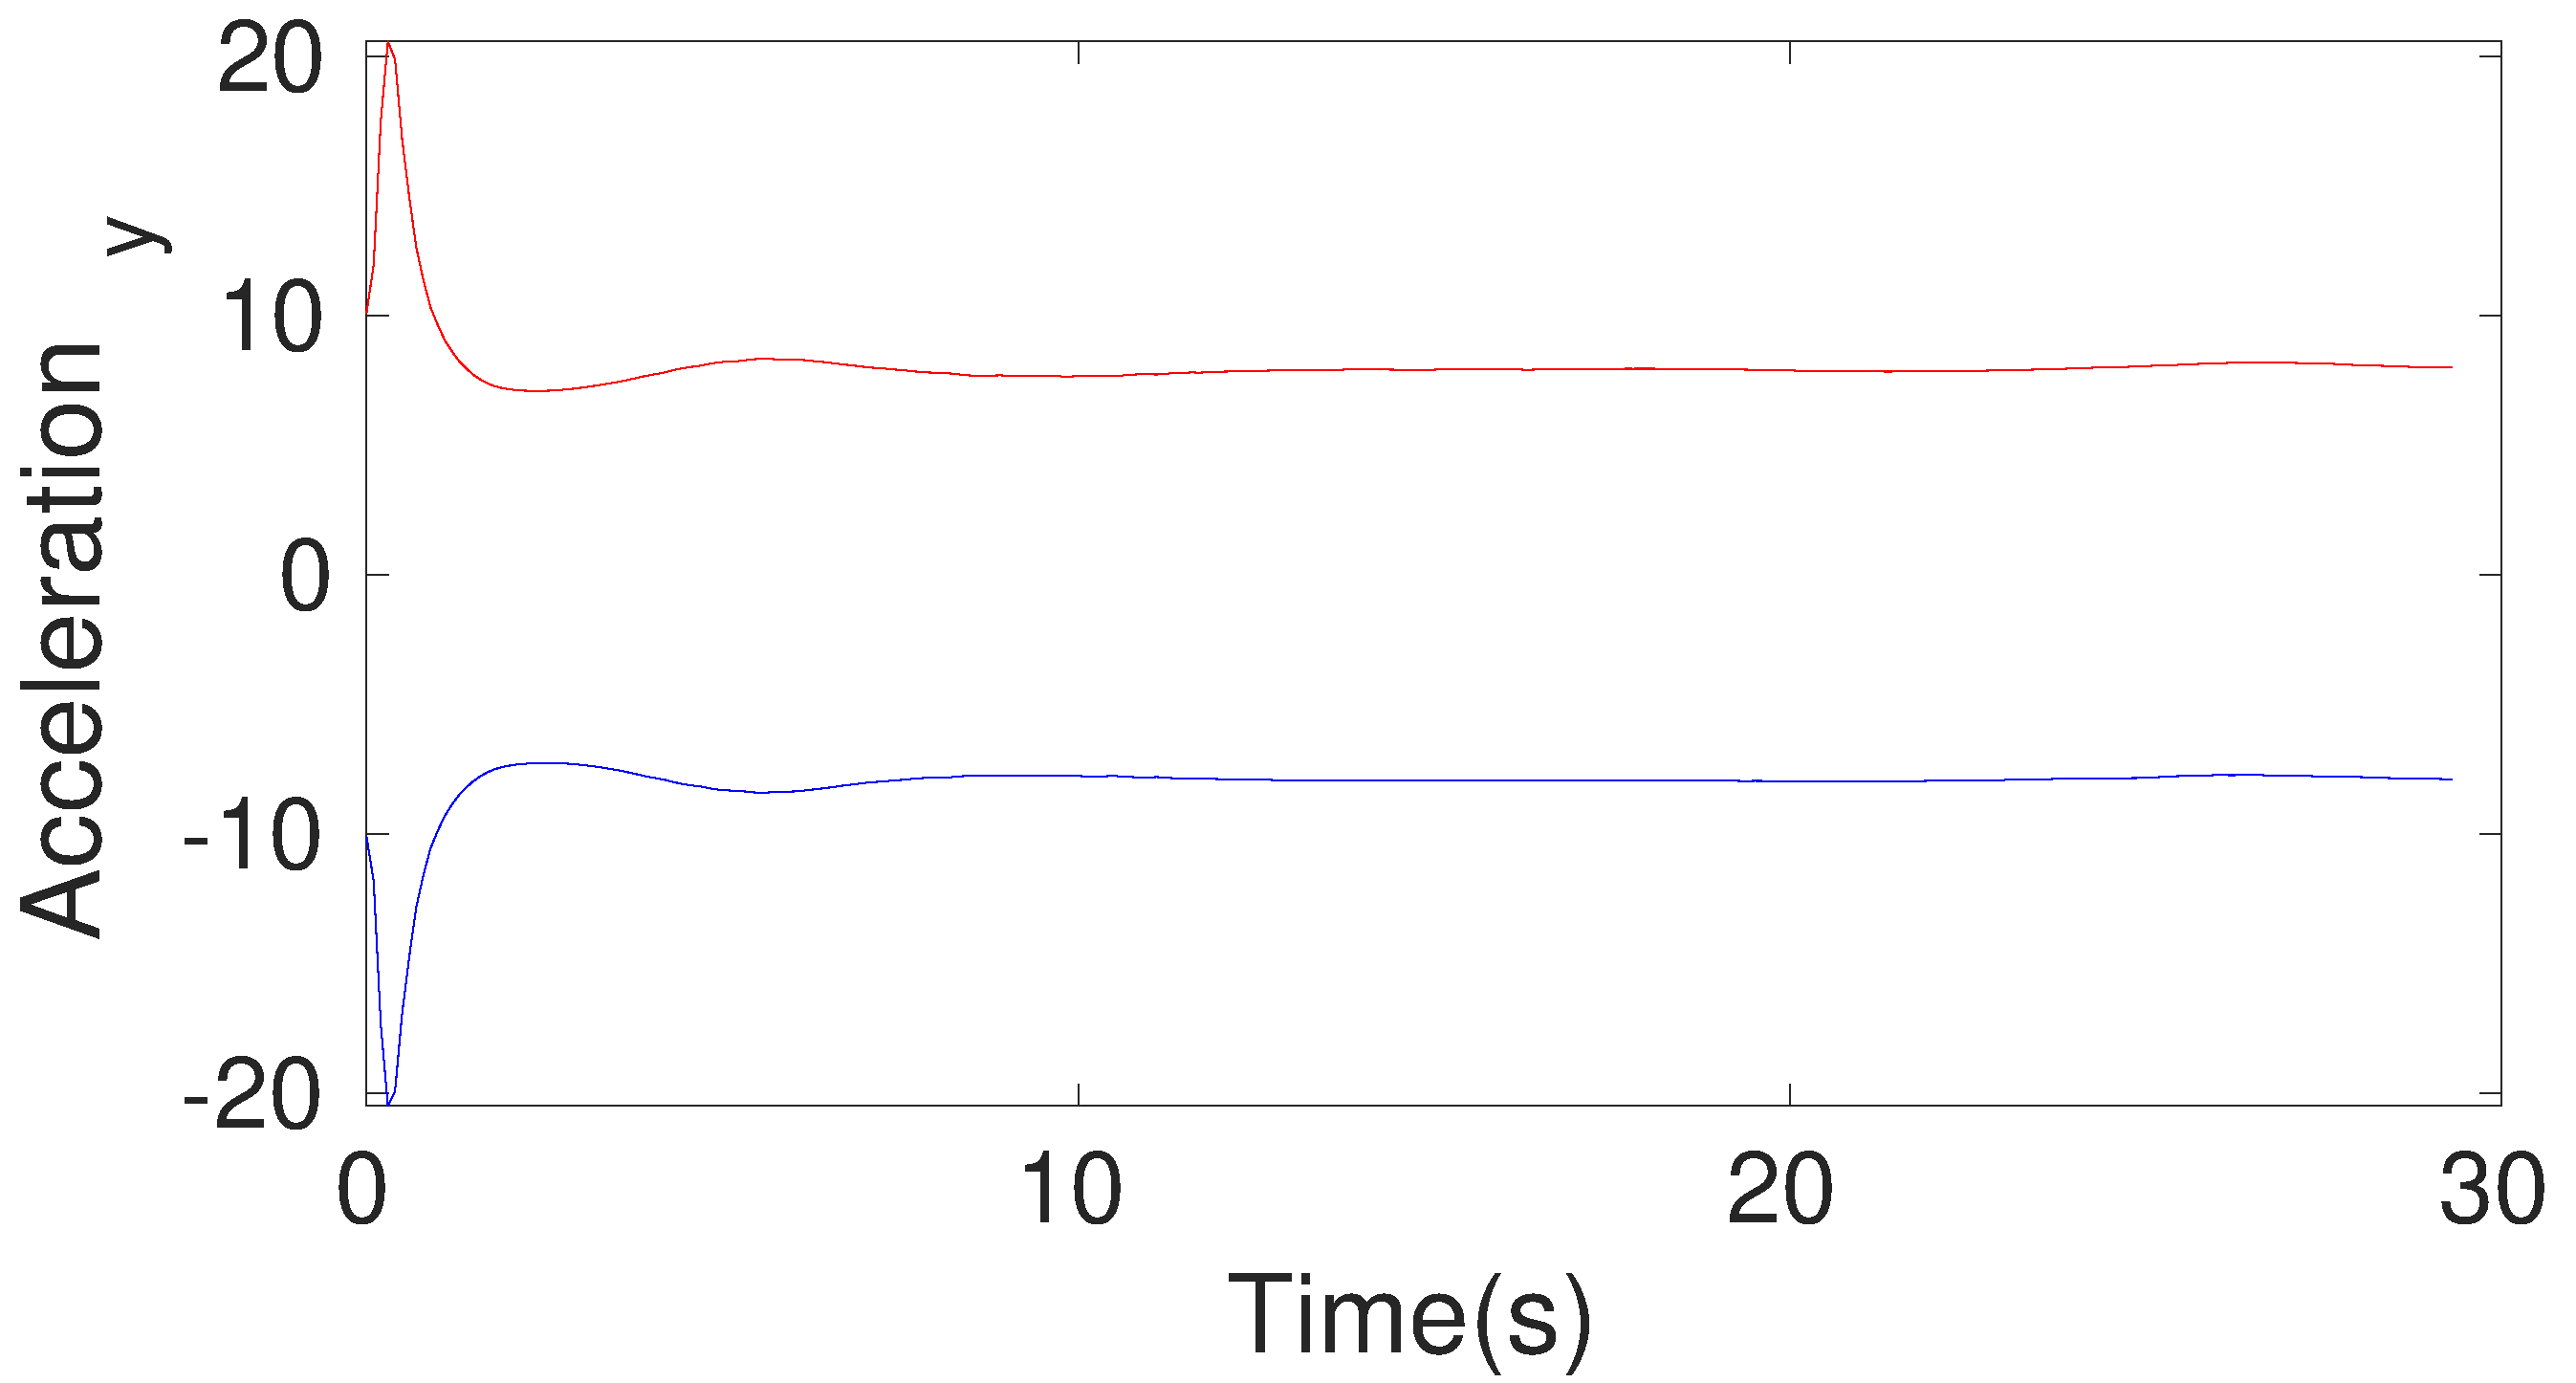
\includegraphics[width=.9\linewidth]{figures/Frad/s3caSMAcceleration_y}
\end{subfigure}
\caption{Estimation using Constant Acceleration}
\end{figure}

\begin{figure}[h]
\begin{subfigure}{.5\linewidth}
\centering
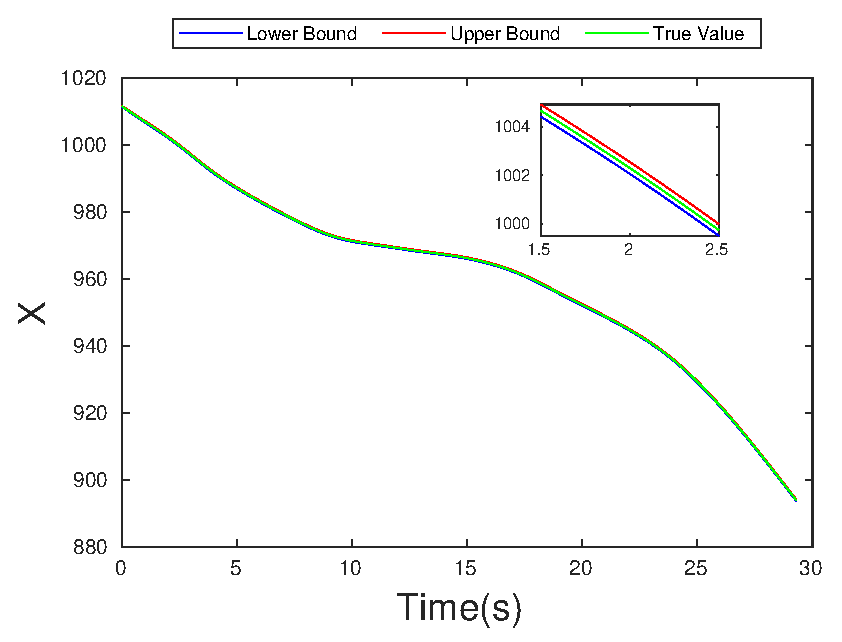
\includegraphics[width=\linewidth]{figures/Frad/s3csSMX}
\end{subfigure}
\begin{subfigure}{.5\linewidth}
\centering
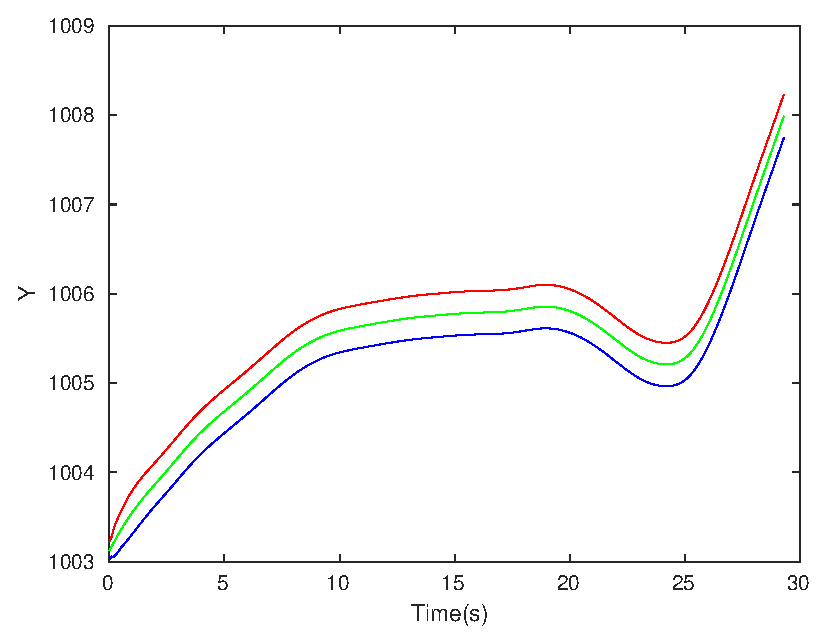
\includegraphics[width=\linewidth]{figures/Frad/s3csSMY}
\end{subfigure}
\begin{subfigure}{.5\linewidth}
\centering
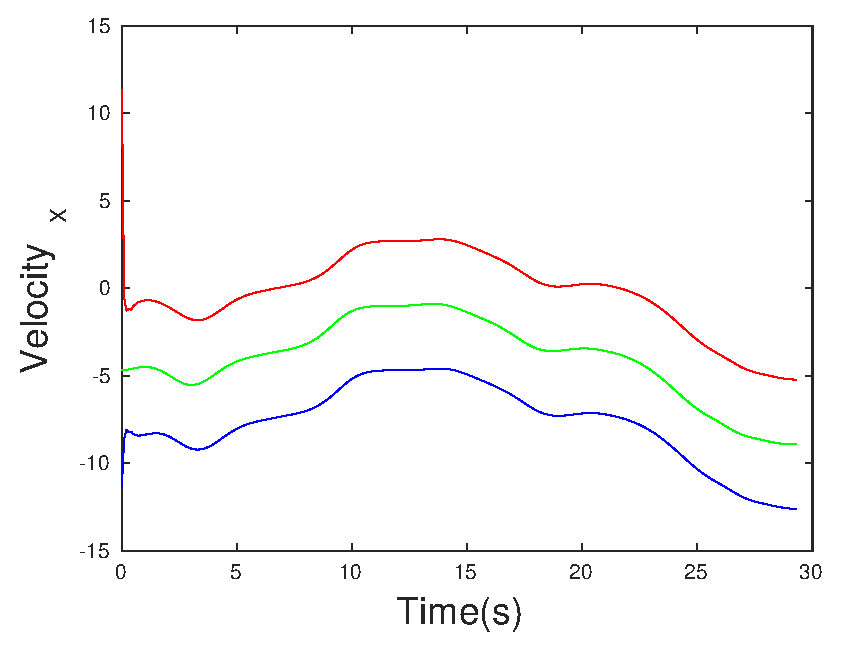
\includegraphics[width=.9\linewidth]{figures/Frad/s3csSMVelocity_x}
\end{subfigure}
\begin{subfigure}{.5\linewidth}
\centering
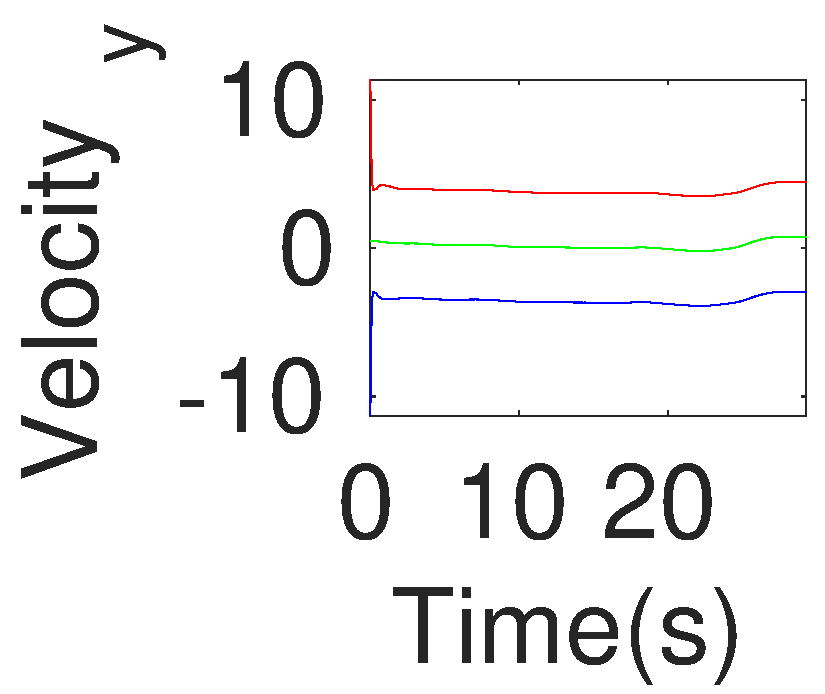
\includegraphics[width=.9\linewidth]{figures/Frad/s3csSMVelocity_y}
\end{subfigure}
\begin{subfigure}{.5\linewidth}
\centering
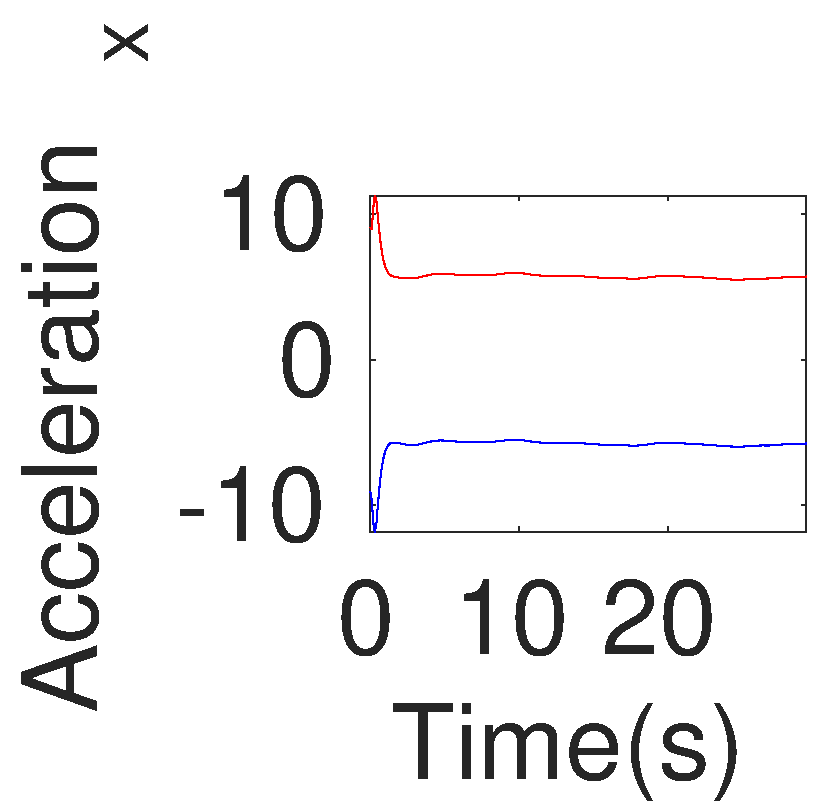
\includegraphics[width=.9\linewidth]{figures/Frad/s3csSMAcceleration_x}
\end{subfigure}
\begin{subfigure}{.5\linewidth}
\centering
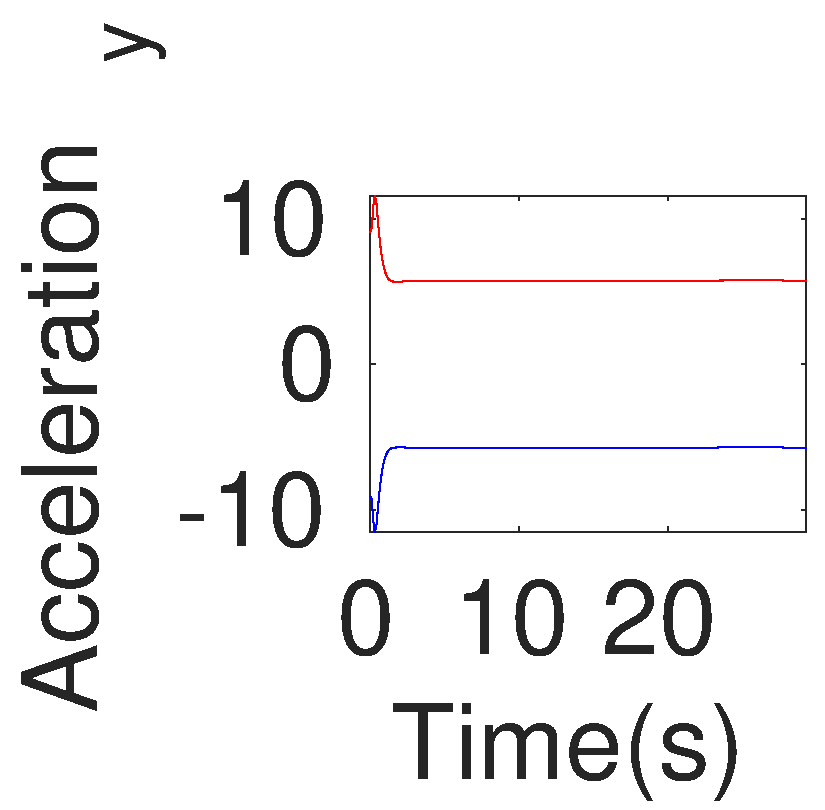
\includegraphics[width=.9\linewidth]{figures/Frad/s3csSMAcceleration_y}
\end{subfigure}
\caption{Estimation using Singer Acceleration}
\end{figure}


\subsection{Segment Minimization using P-Radius}
\begin{figure}[h]
\begin{subfigure}{.5\linewidth}
\centering
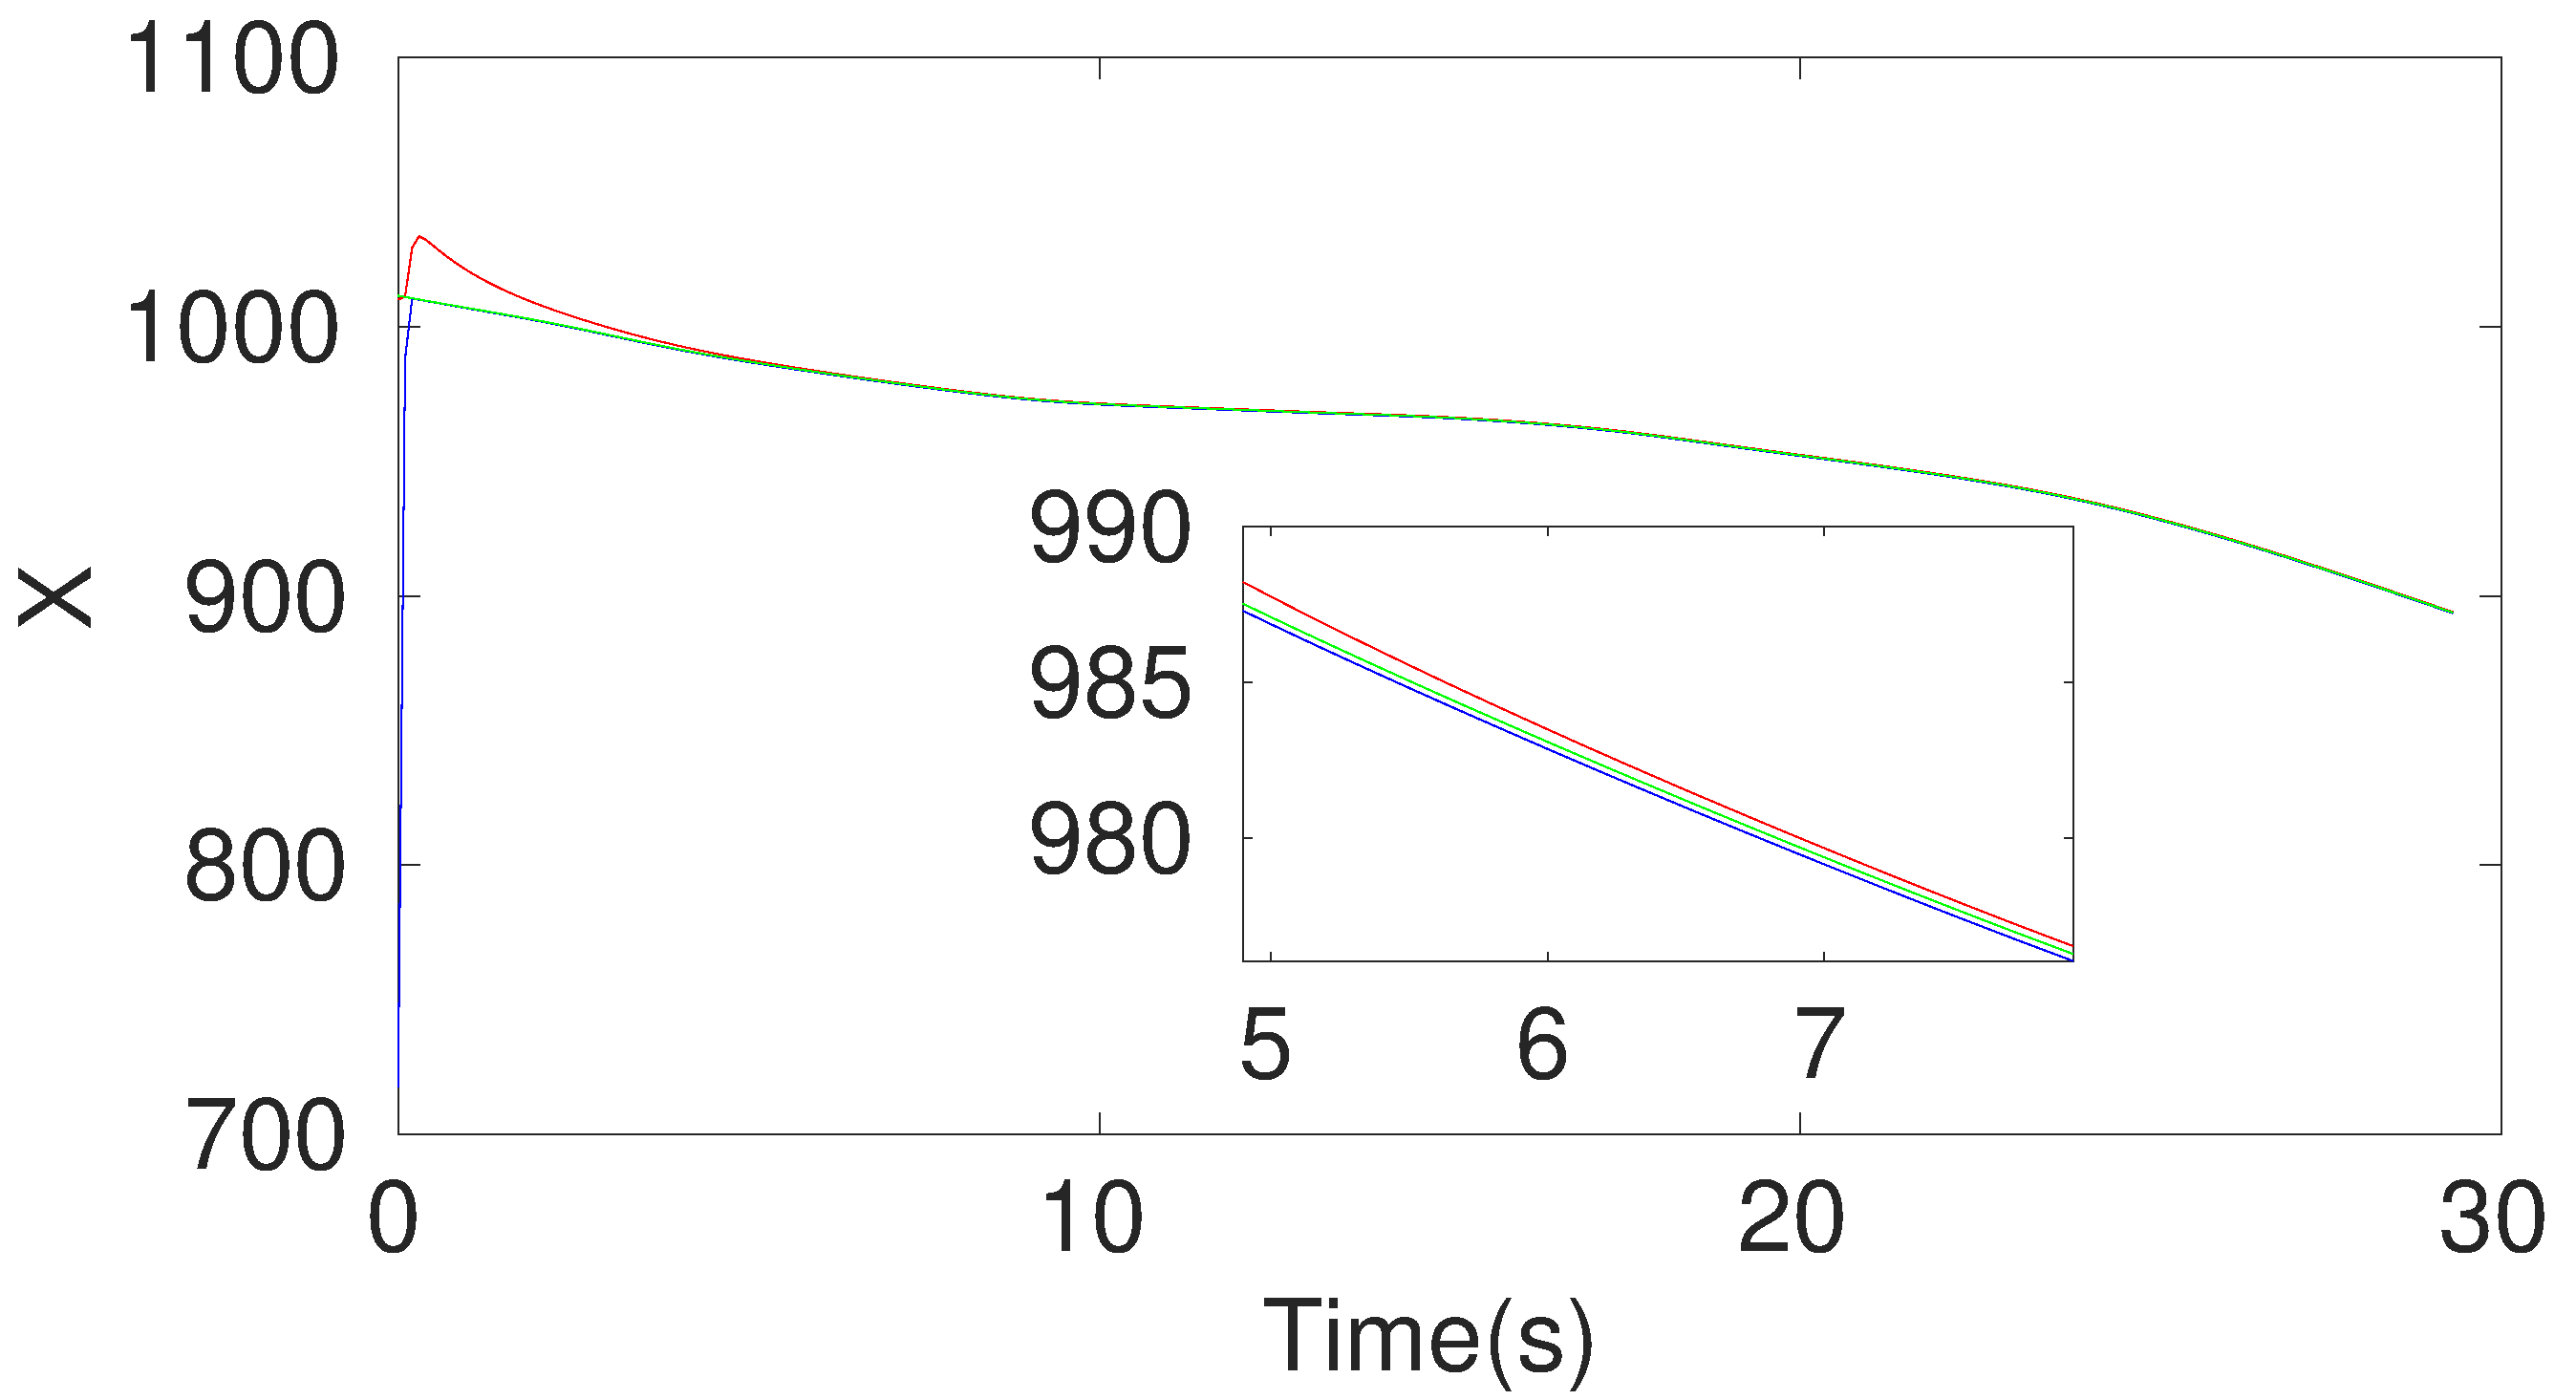
\includegraphics[width=\linewidth]{figures/Prad/s3cvpradX}
\end{subfigure}
\begin{subfigure}{.5\linewidth}
\centering
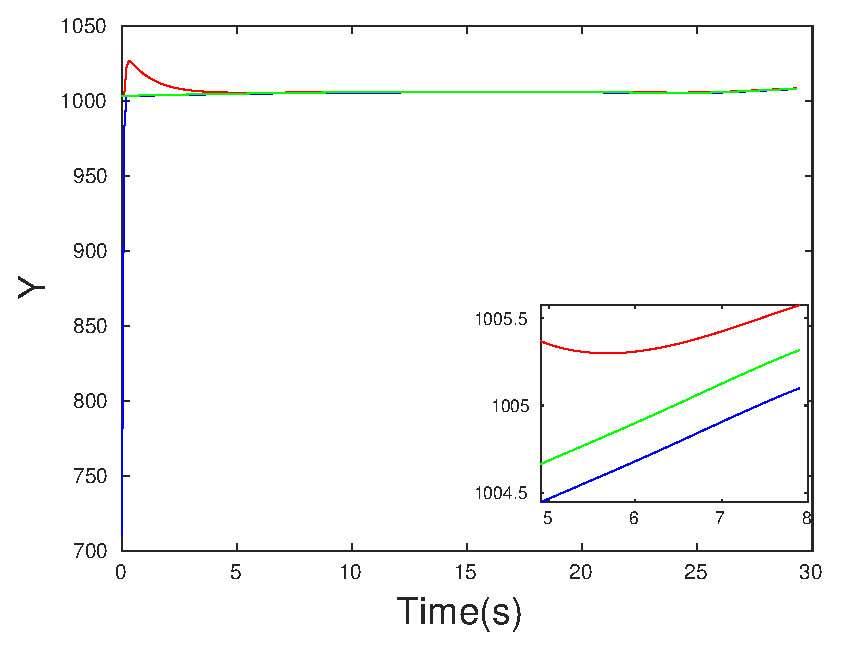
\includegraphics[width=\linewidth]{figures/Prad/s3cvpradY}
\end{subfigure}
\begin{subfigure}{.5\linewidth}
\centering
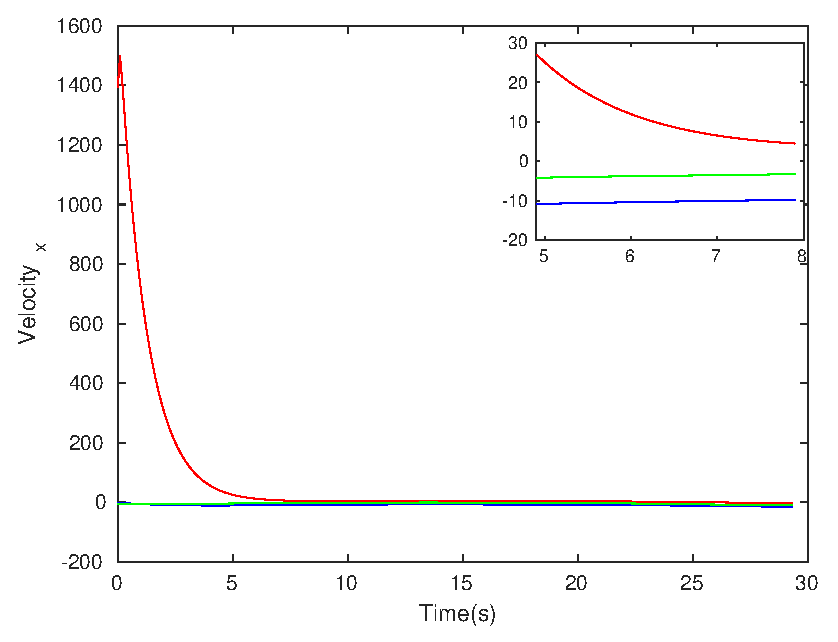
\includegraphics[width=.9\linewidth]{figures/Prad/s3cvpradVelocity_x}
\end{subfigure}
\begin{subfigure}{.5\linewidth}
\centering
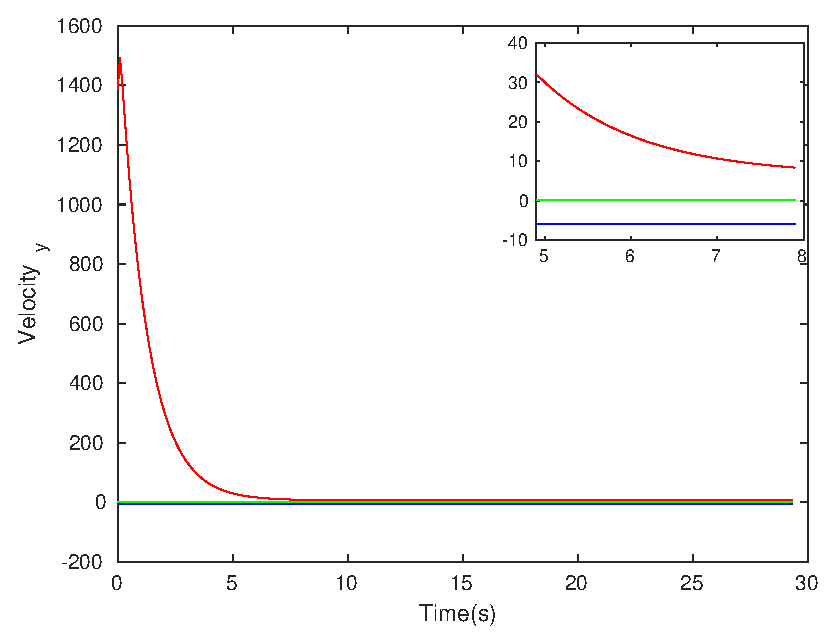
\includegraphics[width=.9\linewidth]{figures/Prad/s3cvpradVelocity_y}
\end{subfigure}
\caption{Estimation using Constant Velocity}
\end{figure}

\begin{figure}[h]
\begin{subfigure}{.5\linewidth}
\centering
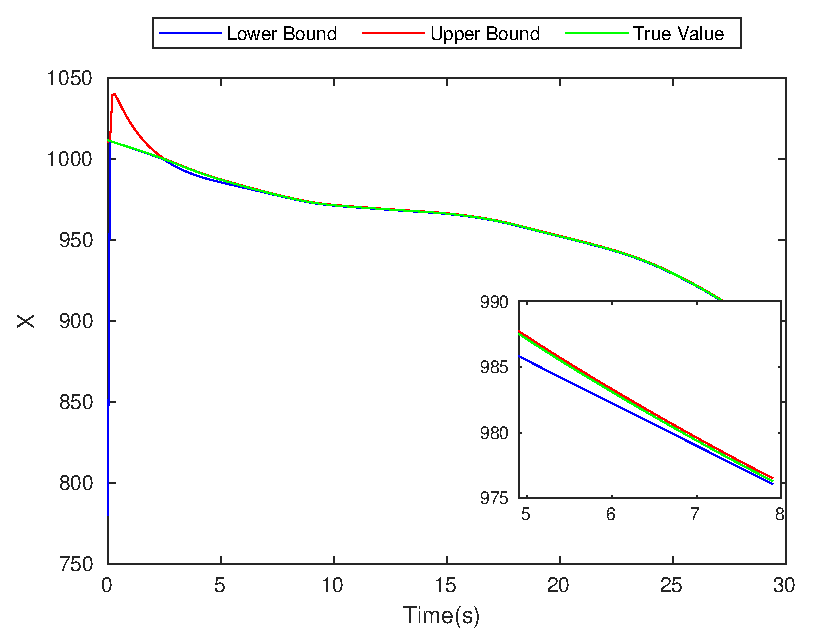
\includegraphics[width=\linewidth]{figures/Prad/s3capradX}
\end{subfigure}
\begin{subfigure}{.5\linewidth}
\centering
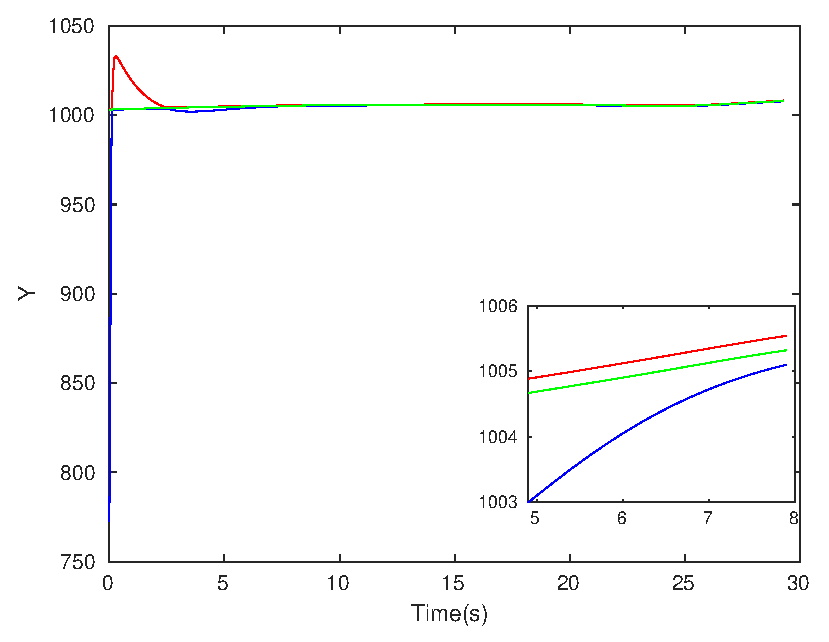
\includegraphics[width=\linewidth]{figures/Prad/s3capradY}
\end{subfigure}
\begin{subfigure}{.5\linewidth}
\centering
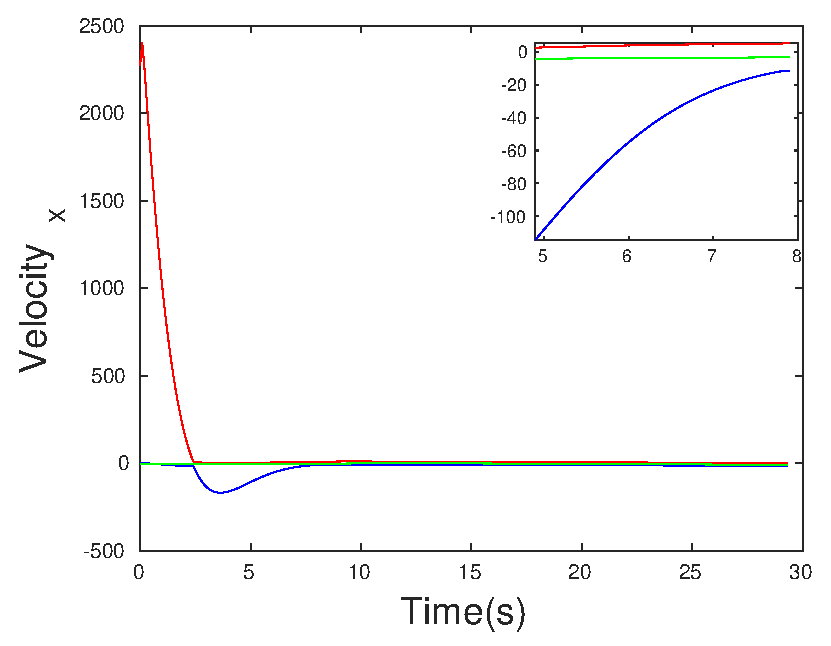
\includegraphics[width=.9\linewidth]{figures/Prad/s3capradVelocity_x}
\end{subfigure}
\begin{subfigure}{.5\linewidth}
\centering
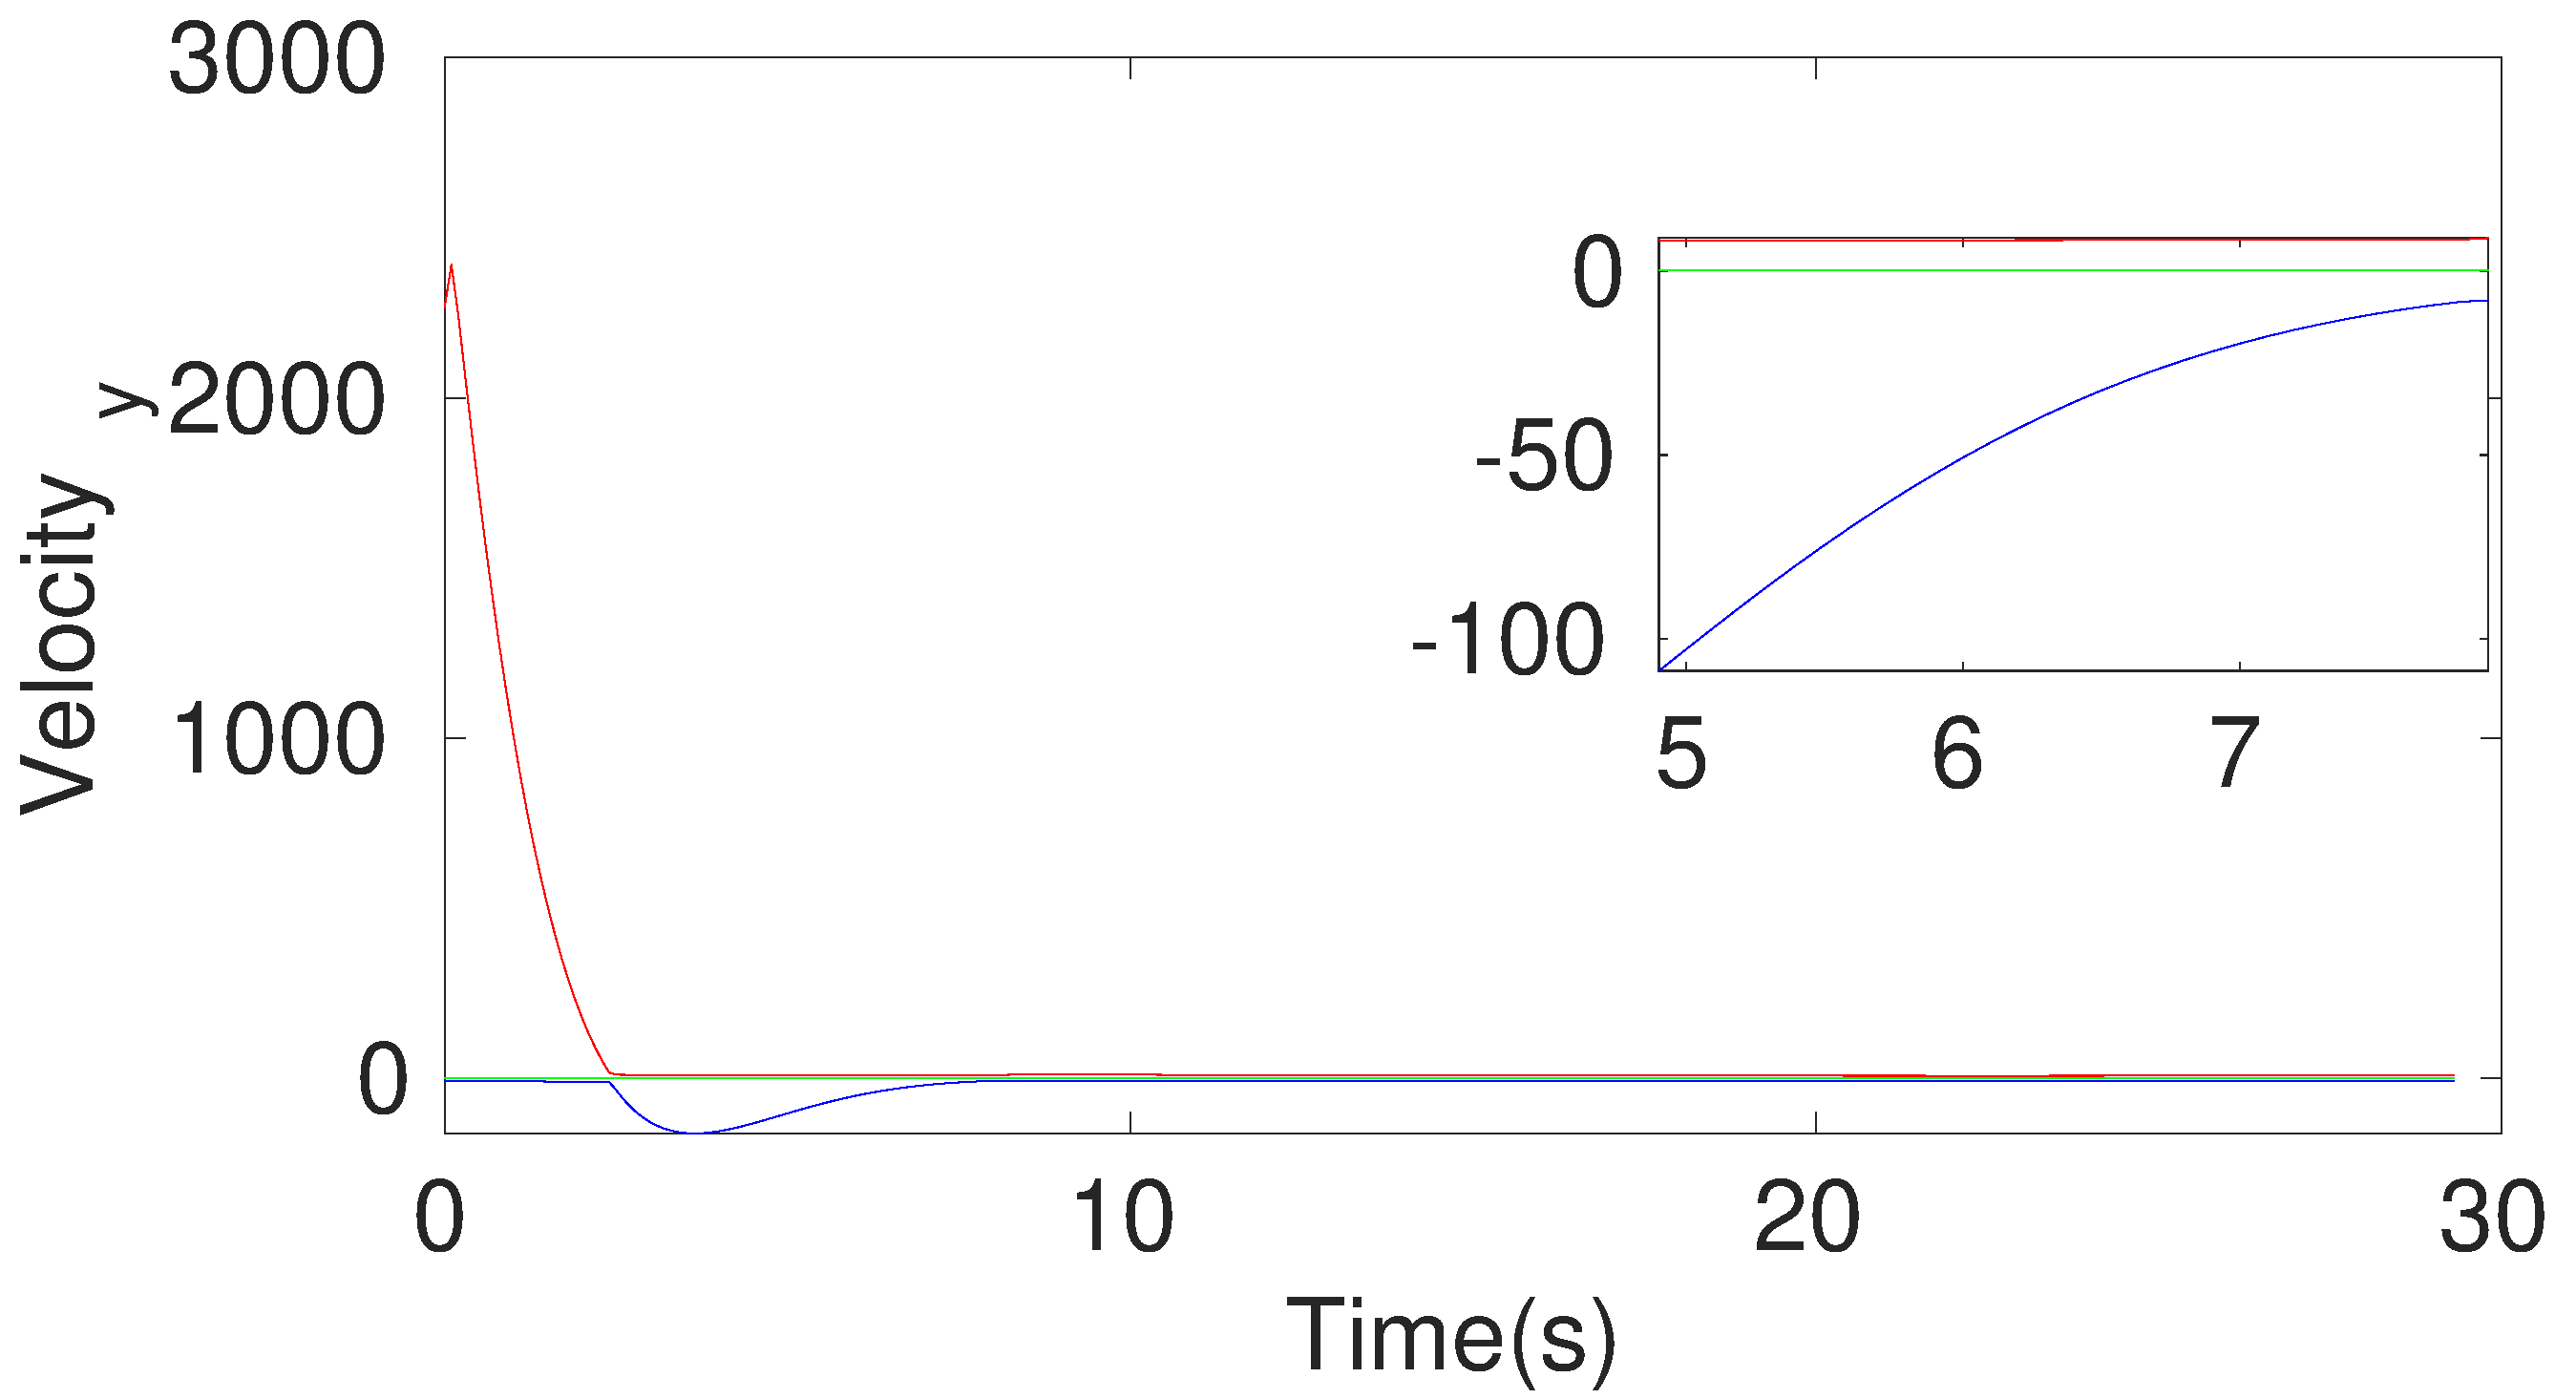
\includegraphics[width=.9\linewidth]{figures/Prad/s3capradVelocity_y}
\end{subfigure}
\begin{subfigure}{.5\linewidth}
\centering
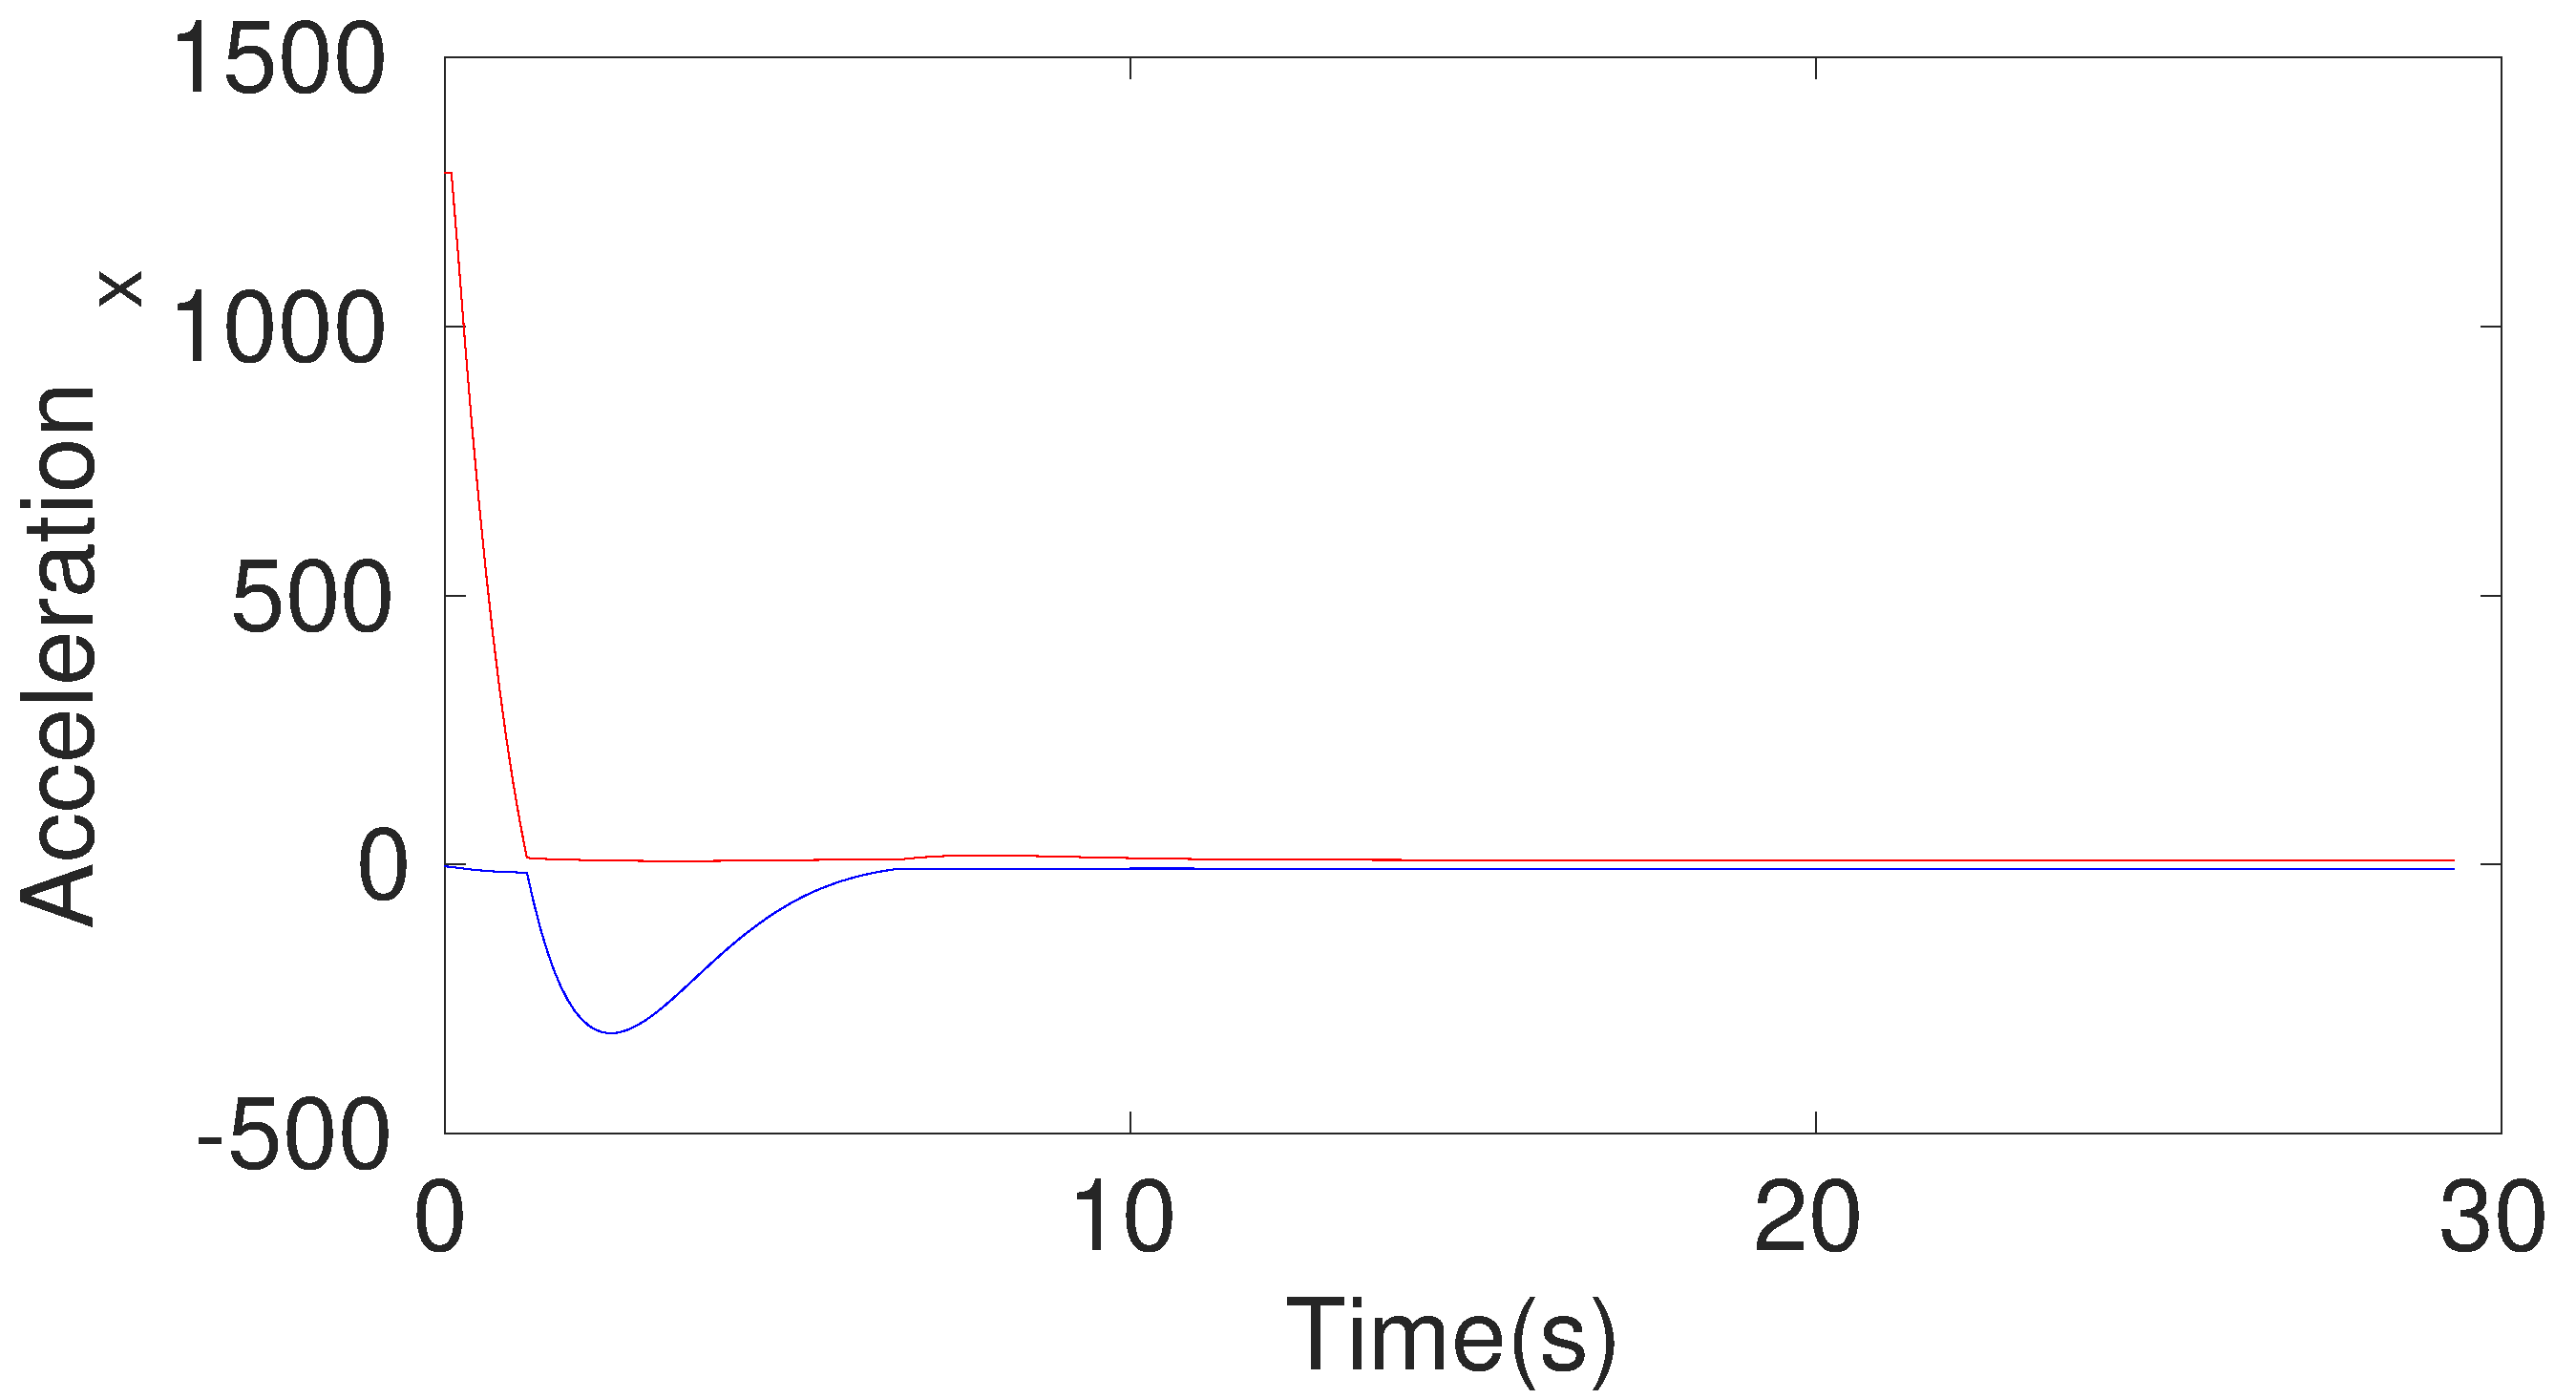
\includegraphics[width=.9\linewidth]{figures/Prad/s3capradAcceleration_x}
\end{subfigure}
\begin{subfigure}{.5\linewidth}
\centering
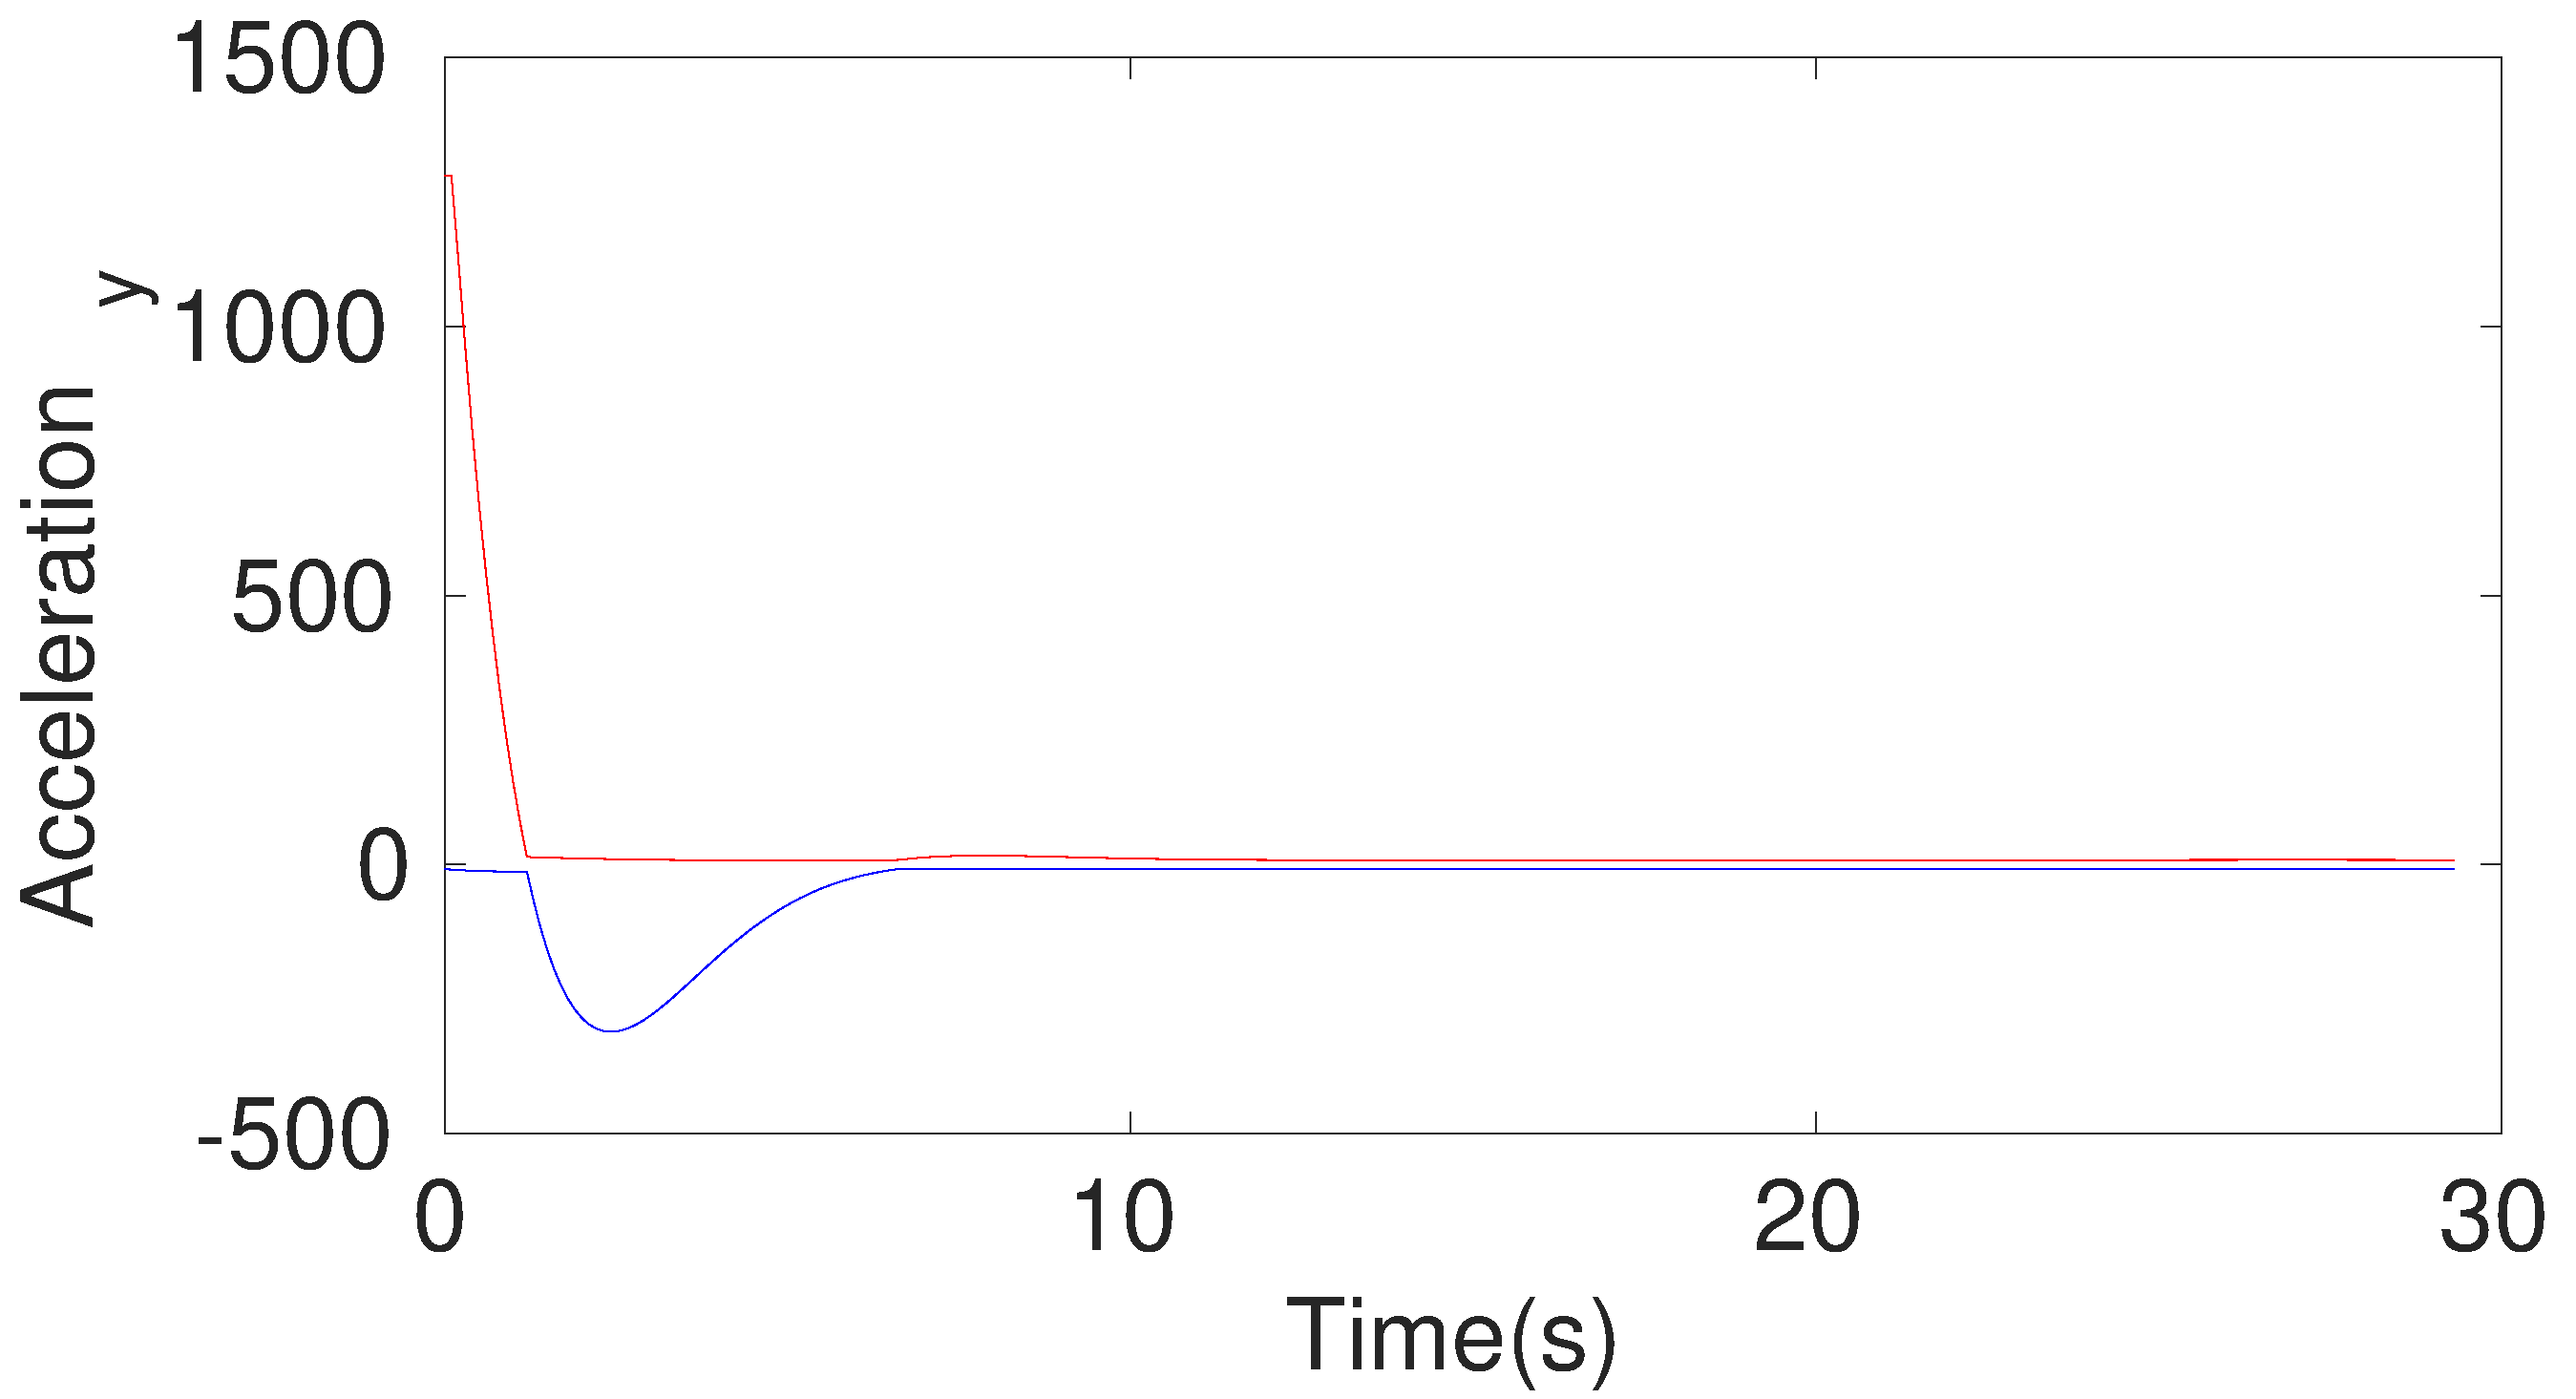
\includegraphics[width=.9\linewidth]{figures/Prad/s3capradAcceleration_y}
\end{subfigure}
\caption{Estimation using Constant Acceleration}
\end{figure}
\begin{figure}[h]
\begin{subfigure}{.5\linewidth}
\centering
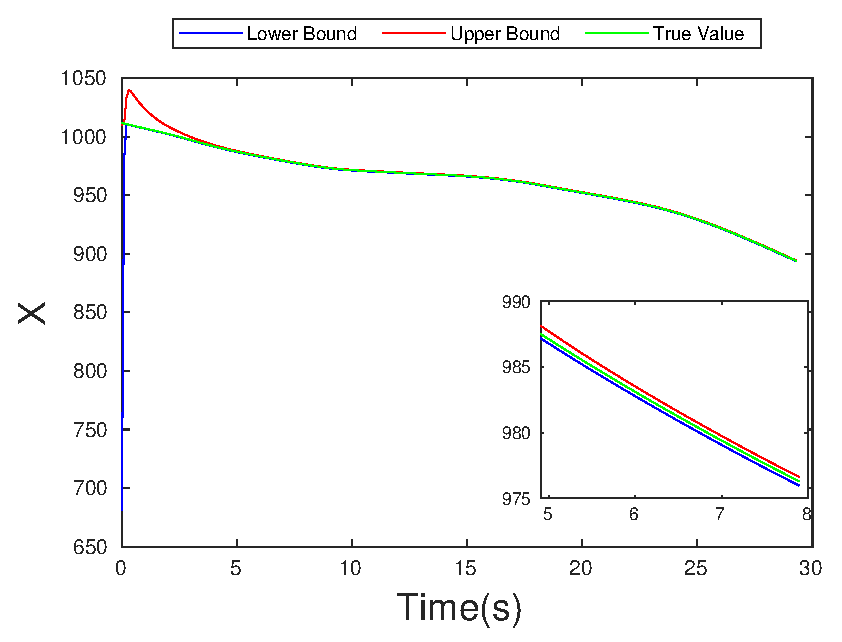
\includegraphics[width=\linewidth]{figures/Prad/s3cspradX}
\end{subfigure}
\begin{subfigure}{.5\linewidth}
\centering
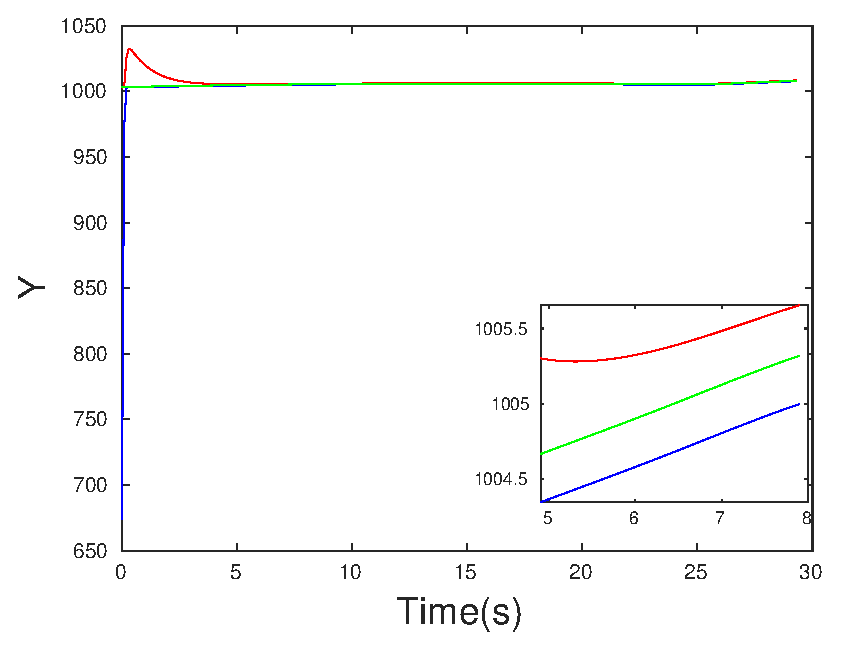
\includegraphics[width=\linewidth]{figures/Prad/s3cspradY}
\end{subfigure}
\begin{subfigure}{.5\linewidth}
\centering
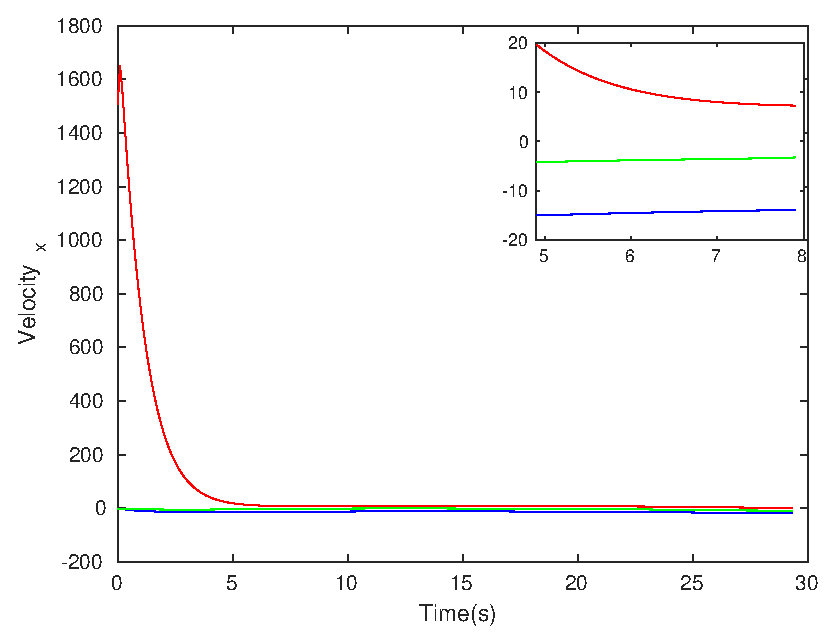
\includegraphics[width=.9\linewidth]{figures/Prad/s3cspradVelocity_x}
\end{subfigure}
\begin{subfigure}{.5\linewidth}
\centering
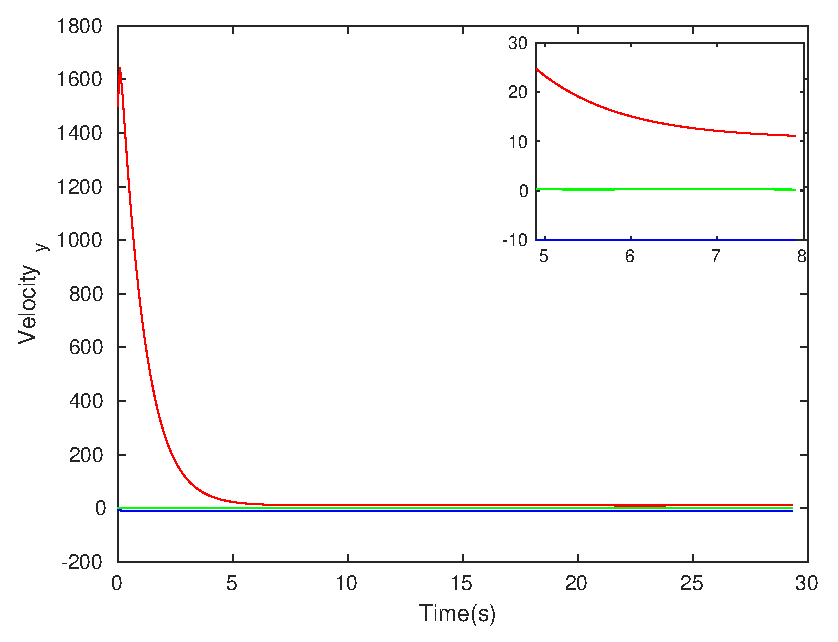
\includegraphics[width=.9\linewidth]{figures/Prad/s3cspradVelocity_y}
\end{subfigure}
\begin{subfigure}{.5\linewidth}
\centering
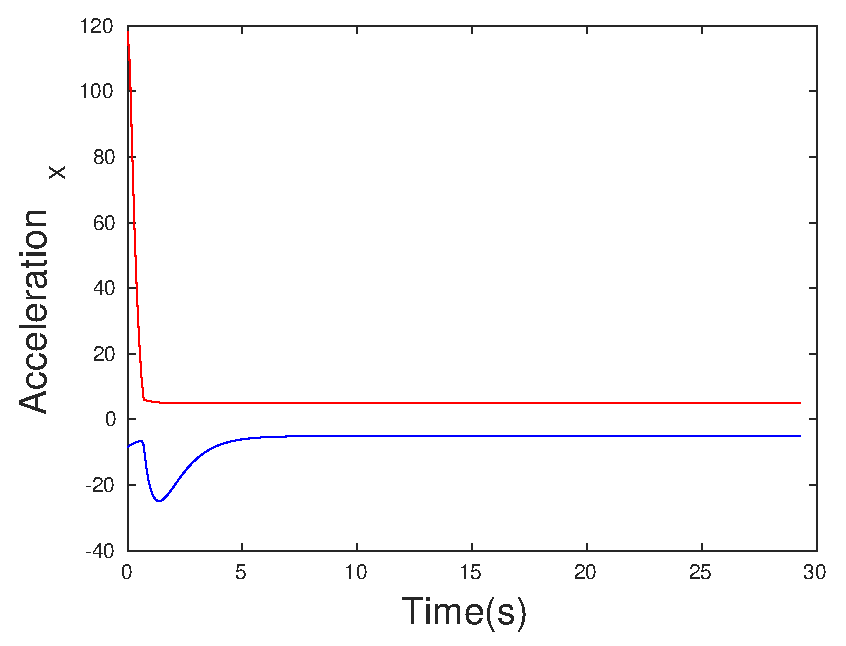
\includegraphics[width=.9\linewidth]{figures/Prad/s3cspradAcceleration_x}
\end{subfigure}
\begin{subfigure}{.5\linewidth}
\centering
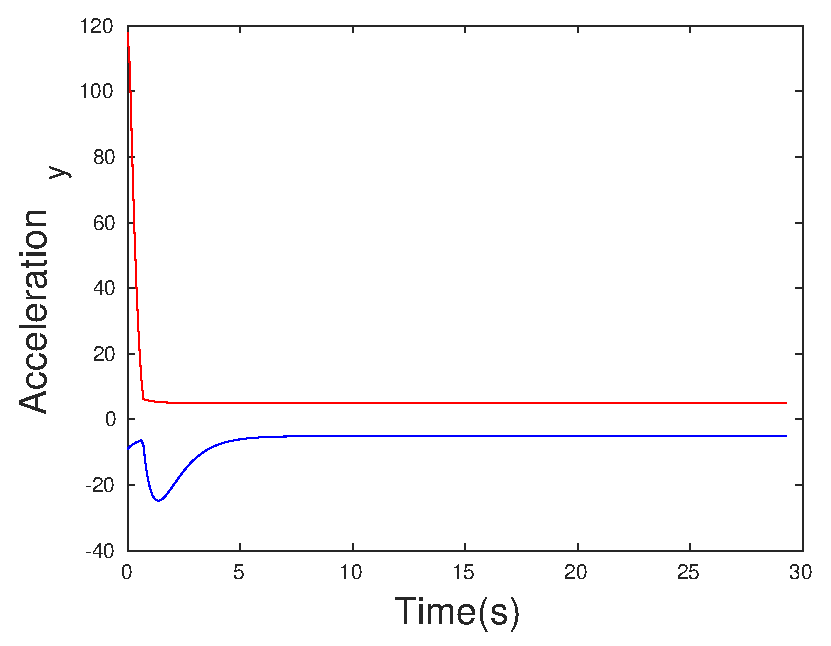
\includegraphics[width=.9\linewidth]{figures/Prad/s3cspradAcceleration_y}
\end{subfigure}
\caption{Estimation using Singer Acceleration}
\end{figure}



\subsection{Segment Minimization using H-$\infty$}
\FloatBarrier
\begin{figure}[h]
\begin{subfigure}{.5\linewidth}
\centering
\includegraphics[width=\linewidth]{figures/HInf/s3cvHInfX}
\end{subfigure}
\begin{subfigure}{.5\linewidth}
\centering
\includegraphics[width=\linewidth]{figures/HInf/s3cvHInfY}
\end{subfigure}
\begin{subfigure}{.5\linewidth}
\centering
\includegraphics[width=.9\linewidth]{figures/HInf/s3cvHInfVelocity_x}
\end{subfigure}
\begin{subfigure}{.5\linewidth}
\centering
\includegraphics[width=.9\linewidth]{figures/HInf/s3cvHInfVelocity_y}
\end{subfigure}
\caption{Estimation using Constant Velocity}
\end{figure}

\begin{figure}[h]
\begin{subfigure}{.5\linewidth}
\centering
\includegraphics[width=\linewidth]{figures/HInf/s3caHInfX}
\end{subfigure}
\begin{subfigure}{.5\linewidth}
\centering
\includegraphics[width=\linewidth]{figures/HInf/s3caHInfY}
\end{subfigure}
\begin{subfigure}{.5\linewidth}
\centering
\includegraphics[width=.9\linewidth]{figures/HInf/s3caHInfVelocity_x}
\end{subfigure}
\begin{subfigure}{.5\linewidth}
\centering
\includegraphics[width=.9\linewidth]{figures/HInf/s3caHInfVelocity_y}
\end{subfigure}
\begin{subfigure}{.5\linewidth}
\centering
\includegraphics[width=.9\linewidth]{figures/HInf/s3caHInfAcceleration_x}
\end{subfigure}
\begin{subfigure}{.5\linewidth}
\centering
\includegraphics[width=.9\linewidth]{figures/HInf/s3caHInfAcceleration_y}
\end{subfigure}
\caption{Estimation using Constant Acceleration}
\end{figure}



\begin{figure}[h]
\begin{subfigure}{.5\linewidth}
\centering
\includegraphics[width=\linewidth]{figures/HInf/s3csHInfX}
\end{subfigure}
\begin{subfigure}{.5\linewidth}
\centering
\includegraphics[width=\linewidth]{figures/HInf/s3csHInfY}
\end{subfigure}
\begin{subfigure}{.5\linewidth}
\centering
\includegraphics[width=.9\linewidth]{figures/HInf/s3csHInfVelocity_x}
\end{subfigure}
\begin{subfigure}{.5\linewidth}
\centering
\includegraphics[width=.9\linewidth]{figures/HInf/s3csHInfVelocity_y}
\end{subfigure}
\begin{subfigure}{.5\linewidth}
\centering
\includegraphics[width=.9\linewidth]{figures/HInf/s3csHInfAcceleration_x}
\end{subfigure}
\begin{subfigure}{.5\linewidth}
\centering
\includegraphics[width=.9\linewidth]{figures/HInf/s3csHInfAcceleration_y}
\end{subfigure}
\caption{Estimation using Singer Acceleration}
\end{figure}


\section{Rate of Change of Bounds}
\FloatBarrier
\subsection{Constant Velocity}
\begin{figure}[!h]
\begin{subfigure}{.5\linewidth}
\centering
\includegraphics[width=\linewidth]{figures/BoundChange/CV/cv_bound_changeX}
\end{subfigure}
\begin{subfigure}{.5\linewidth}
\centering
\includegraphics[width=\linewidth]{figures/BoundChange/CV/cv_bound_changeY}
\end{subfigure}
\begin{subfigure}{.5\linewidth}
\centering
\includegraphics[width=.9\linewidth]{figures/BoundChange/CV/cv_bound_changeVelocity_x}
\end{subfigure}
\begin{subfigure}{.5\linewidth}
\centering
\includegraphics[width=.9\linewidth]{figures/BoundChange/CV/cv_bound_changeVelocity_y}
\end{subfigure}
\caption{Rate of change of bounds}
\end{figure}

\subsection{Constant Acceleration}
\FloatBarrier
\begin{figure}[!h]
\begin{subfigure}{.5\linewidth}
\centering
\includegraphics[width=\linewidth]{figures/BoundChange/CA/ca_bound_changeX}
\end{subfigure}
\begin{subfigure}{.5\linewidth}
\centering
\includegraphics[width=\linewidth]{figures/BoundChange/CA/ca_bound_changeY}
\end{subfigure}
\begin{subfigure}{.5\linewidth}
\centering
\includegraphics[width=.9\linewidth]{figures/BoundChange/CA/ca_bound_changeVelocity_x}
\end{subfigure}
\begin{subfigure}{.5\linewidth}
\centering
\includegraphics[width=.9\linewidth]{figures/BoundChange/CA/ca_bound_changeVelocity_y}
\end{subfigure}
\begin{subfigure}{.5\linewidth}
\centering
\includegraphics[width=.9\linewidth]{figures/BoundChange/CA/ca_bound_changeAcceleration_x}
\end{subfigure}
\begin{subfigure}{.5\linewidth}
\centering
\includegraphics[width=.9\linewidth]{figures/BoundChange/CA/ca_bound_changeAcceleration_y}
\end{subfigure}
\caption{Rate of change of bounds}
\end{figure}

\subsection{Singer Acceleration Model}
\FloatBarrier
\begin{figure}[!h]
\begin{subfigure}{.5\linewidth}
\centering
\includegraphics[width=\linewidth]{figures/BoundChange/CS/cs_bound_changeX}
\end{subfigure}
\begin{subfigure}{.5\linewidth}
\centering
\includegraphics[width=\linewidth]{figures/BoundChange/CS/cs_bound_changeY}
\end{subfigure}
\begin{subfigure}{.5\linewidth}
\centering
\includegraphics[width=.9\linewidth]{figures/BoundChange/CS/cs_bound_changeVelocity_x}
\end{subfigure}
\begin{subfigure}{.5\linewidth}
\centering
\includegraphics[width=.9\linewidth]{figures/BoundChange/CS/cs_bound_changeVelocity_y}
\end{subfigure}
\begin{subfigure}{.5\linewidth}
\centering
\includegraphics[width=.9\linewidth]{figures/BoundChange/CS/cs_bound_changeAcceleration_x}
\end{subfigure}
\begin{subfigure}{.5\linewidth}
\centering
\includegraphics[width=.9\linewidth]{figures/BoundChange/CS/cs_bound_changeAcceleration_y}
\end{subfigure}
\caption{Rate of change of bounds}
\end{figure}
\chapter{Template Code}\label{app:code}
\section{Template for Model}
% This file was automatically created from the m-file 
% "m2tex.m" written by USL. 
% The fontencoding in this file is UTF-8. 
%  
% You will need to include the following two packages in 
% your LaTeX-Main-File. 
%  
% \usepackage{color} 
% \usepackage{fancyvrb} 
%  
% It is advised to use the following option for Inputenc 
% \usepackage[utf8]{inputenc} 
%  
  
% definition of matlab colors: 
\definecolor{mblue}{rgb}{0,0,1} 
\definecolor{mgreen}{rgb}{0.13333,0.5451,0.13333} 
\definecolor{mred}{rgb}{0.62745,0.12549,0.94118} 
\definecolor{mgrey}{rgb}{0.5,0.5,0.5} 
\definecolor{mdarkgrey}{rgb}{0.25,0.25,0.25} 
  
\DefineShortVerb[fontfamily=courier,fontseries=m]{\$} 
\DefineShortVerb[fontfamily=courier,fontseries=b]{\#} 
  
\noindent                            
 $$\color{mblue}$classdef$\color{black}$ Model$\\
 $    $\color{mgreen}$%MODEL Model Template$\color{black}$$\\
 $    $\color{mgreen}$%   dim_x: estimate dimension$\color{black}$$\\
 $    $\color{mgreen}$%   dim_y: measurement dimension$\color{black}$$\\
 $    $\\
 $    properties$\\
 $        A$\\
 $        C$\\
 $        W$\\
 $        V$\\
 $        initial$\\
 $        dim_x;$\\
 $        dim_;$\\
 $        delT = 0.1;$\\
 $    $\color{mblue}$end$\color{black}$$\\
 $    $\\
 $    methods$\\
 $        $\color{mblue}$function$\color{black}$ obj = Model(delT)$\\
 $            $\color{mgreen}$%MODEL Construct an instance of this class$\color{black}$$\\
 $            $\color{mgreen}$%   Initializes the model variables$\color{black}$$\\
 $            obj.delT = delT; $\color{mgreen}$% add the time step$\color{black}$$\\
 $            $\\
 $            $\color{mgreen}$% Assign parameters here$\color{black}$$\\
 $        $\color{mblue}$end$\color{black}$$\\
 $    $\color{mblue}$end$\color{black}$$\\
 $$\color{mblue}$end$\color{black}$$\\
 $$\\
 $$\\ 
  
\UndefineShortVerb{\$} 
\UndefineShortVerb{\#}
\pagebreak
\section{Template for Estimator}
% This file was automatically created from the m-file 
% "m2tex.m" written by USL. 
% The fontencoding in this file is UTF-8. 
%  
% You will need to include the following two packages in 
% your LaTeX-Main-File. 
%  
% \usepackage{color} 
% \usepackage{fancyvrb} 
%  
% It is advised to use the following option for Inputenc 
% \usepackage[utf8]{inputenc} 
%  
  
% definition of matlab colors: 
\definecolor{mblue}{rgb}{0,0,1} 
\definecolor{mgreen}{rgb}{0.13333,0.5451,0.13333} 
\definecolor{mred}{rgb}{0.62745,0.12549,0.94118} 
\definecolor{mgrey}{rgb}{0.5,0.5,0.5} 
\definecolor{mdarkgrey}{rgb}{0.25,0.25,0.25} 
  
\DefineShortVerb[fontfamily=courier,fontseries=m]{\$} 
\DefineShortVerb[fontfamily=courier,fontseries=b]{\#} 
  
\noindent                                     
 $$\color{mblue}$classdef$\color{black}$ Estimator < handle$\\
 $    $\color{mgreen}$%ESTIMATOR Estimator template$\color{black}$$\\
 $    $\color{mgreen}$%   model: model to represent vehicle dynamics$\color{black}$$\\
 $    $\\
 $    properties$\\
 $        model$\\
 $        E$\\
 $        F$\\
 $        x_estimated$\\
 $        index$\\
 $    $\color{mblue}$end$\color{black}$$\\
 $    $\\
 $    methods$\\
 $        $\color{mblue}$function$\color{black}$ obj = Estimator(model)$\\
 $            $\color{mgreen}$%ESTIMATOR Constructor$\color{black}$$\\
 $            $\color{mgreen}$% Initialize variables$\color{black}$$\\
 $            obj.model = model;$\\
 $            obj.index = 1; $\color{mgreen}$% keep track of measurements$\color{black}$$\\
 $            $\\
 $            $\color{mgreen}$% initialize variables here$\color{black}$$\\
 $            $\\
 $            $\color{mgreen}$% implement initial computation $\color{black}$$\\
 $        $\color{mblue}$end$\color{black}$$\\
 $        $\\
 $        $\color{mblue}$function$\color{black}$ [x_lower, x_upper] = estimate(obj, y)$\\
 $            $\color{mgreen}$%ESTIMATE estimate from the measurement$\color{black}$$\\
 $            $\\
 $            $\color{mgreen}$% implement estimator algorithm on measurement, y$\color{black}$$\\
 $            $\\
 $            $\color{mgreen}$% return bounds$\color{black}$$\\
 $            x_lower = 0;$\\
 $            x_upper = 0;$\\
 $        $\color{mblue}$end$\color{black}$$\\
 $        $\\
 $    $\color{mblue}$end$\color{black}$$\\
 $$\color{mblue}$end$\color{black}$$\\
 $$\\ 
  
\UndefineShortVerb{\$} 
\UndefineShortVerb{\#}
%\end{appendices}

%\microtypesetup{protrusion=false}
% \glsaddall{} % add all defined terms to glossary, even if not referenced in text
% \printglossaries{} % TODO: uncomment if glossary needed
\listoffigures{}
\listoftables{}
\printbibliography{}

\end{document}